%================================================================
% SLO
%----------------------------------------------------------------
% datoteka: 	thesis_template.tex
%
% opis: 		predloga za pisanje diplomskega dela v formatu LaTeX na
% 				Univerza v Ljubljani, Fakulteti za računalništvo in informatiko
%
% pripravili: 	Matej Kristan, Zoran Bosnić, Andrej Čopar,
%			  	po začetni predlogi Gašperja Fijavža
%
% popravil: 	Domen Rački, Jaka Cikač, Matej Kristan
%
% verzija: 		30. september 2016 (dodan razširjeni povzetek)
%================================================================


%================================================================
% SLO: definiraj strukturo dokumenta
% ENG: define file structure
%================================================================
\documentclass[a4paper, 12pt]{book}
\usepackage{longtable}
\usepackage{multirow}
\usepackage{afterpage}
\usepackage{adjustbox}
\usepackage{graphicx} % http://ctan.org/pkg/graphicx
\usepackage{booktabs} % http://ctan.org/pkg/booktabs
\usepackage{xparse}   % http://ctan.org/pkg/xparse
\usepackage{emptypage}
\usepackage{listings}
\usepackage{setspace}
\usepackage{color}
\usepackage{minted}
\usepackage{fontspec}

% set font for source code and urls
\setmonofont{Ubuntu Mono}

% minted settings
\usemintedstyle{tango}
\setminted[python]{xleftmargin=0.5cm}

\NewDocumentCommand{\rot}{O{45} O{1em} m}{\makebox[#2][l]{\rotatebox{#1}{#3}}}%



% foot note
\makeatletter
\newcommand\footnoteref[1]{\protected@xdef\@thefnmark{\ref{#1}}\@footnotemark}
\makeatother


%================================================================
% SLO: Odkomentiraj "\SLOtrue " za izbiro slovenskega jezika
% ENG: Uncomment "\SLOfalse" to chose English languagge
%================================================================
\newif\ifSLO
% switch language

\SLOtrue % Enables Slovenian language
%\SLOfalse  % Enables English language

%================================================================
% SLO: vključi oblikovanje in pakete
% ENG: include design and packages
%================================================================
%----------------------------------------------------------------
% SLO: LaTeX paketi
% ENG: LateX packages
%----------------------------------------------------------------
% SLO: omogoča uporabo slovenskih (latinskih) črk kodiranih v formatu UTF-8
% ENG: enables the use of slovene (latin) caracters encoded in the UFT-8 format
\usepackage[utf8x]{inputenc}
%\inputencoding{utf8} 
% SLO: naloži, med drugim, slovenske delilne vzorce
% ENG: loads, among others, slovene dividing patterns
\usepackage[slovene,english]{babel} 
% SLO: poskrbi za postavitev strani
% ENG: takes care of the page layout
\usepackage{fancyhdr}
% SLO: za vlaganje slik različnih formatov
% ENG: for loading figures of different formats
\usepackage{graphicx}
\usepackage{caption}
\captionsetup[figure]{labelfont=bf} % SLO: napis "Slika #" v krepkem tisku
									% ENG: wirte "Figure #" caption in bold
\captionsetup[table]{labelfont=bf} % SLO: napis "Tabela #" v krepkem tisku
								   % ENG: wirte "Table #" caption in bold

% SLO: za pisanje psevdokode
% ENG: for writing pseudocode
\usepackage{algorithm}
\usepackage{algorithmic}
\floatname{algorithm}{\footnotesize Algorithm} % SLO: napis "Algoritem #" v krepkem tisku
											   % ENG: write "Algorithm #" caption in bold
% SLO: poveže reference slik/tabel in slike/tabele znotraj dokumenta
% ENG: links image/table references with the images/tables within the document
\usepackage{hyperref}
% SLO: pri kliku na referenco slike/tabele se postavi na vrh slike/tabele
% ENG: when clicking the image/table reference, position the focus on top of the image/table
\usepackage[all]{hypcap}
% SLO: omogoča, med drugim, definicjo in uporebo barve
% ENG: enables, among others, the definition and use of colors
\usepackage{xcolor}
%----------------------------------------------------------------
% SLO: dodatni paketi
% ENG: additional packages
%----------------------------------------------------------------
% SLO: omogoča večjo manipulacijo nad tabelami
% ENG: allows for greater manipulation of tables
\usepackage{booktabs}
% SLO: naloži dodatne simbole
% ENG: loads additional symbols
\usepackage{amssymb} 
% SLO: omogoča, med drugim, sklicevanje na formule z eqref
% ENG: enables, among others, equation referencing with eqref
\usepackage{amsmath}
% SLO: omogoča komentiranje večjega dela teksta
% ENG: enables the commenting of larger text parts
\usepackage{verbatim}
% SLO: omogoča rotacijo PDF strani v ležeč položaj
% ENG: enables the rotation of a PDF page to landscape
\usepackage{pdflscape}
% SLO: omogoča barvanje vrstic in stolpcev tabel
% ENG: enables coloring of table rows and columns
\usepackage{colortbl}

\usepackage{url}


%================================================================
% SLO: nastavitve dokumenta
% ENG: document properties
%================================================================
% SLO: prilagoditev robov za tisk
% ENG: margin adjustments for printing
\addtolength{\marginparwidth}{-20pt}
\addtolength{\oddsidemargin}{40pt}
\addtolength{\evensidemargin}{-40pt}
% SLO: razmik med vrsticami
% ENG: line spacing
\renewcommand{\baselinestretch}{1.3} 
% SLO: postavitev strani
% ENG: page layout
\renewcommand{\chaptermark}[1]{\markboth{\MakeUppercase{\thechapter.\ #1}}{}} 
\renewcommand{\sectionmark}[1]{\markright{\MakeUppercase{\thesection.\ #1}}} 
\renewcommand{\headrulewidth}{0.5pt} % Header rule
\renewcommand{\footrulewidth}{0pt} % Footer rule
%
\fancypagestyle{frontmatter}{%
	\fancyhf{} % Clear all headers and footers first
	\fancyhead[LE, RO]{\sl \thepage} 
	%\fancyhead[LO]{\sl \rightmark} 
	%\fancyhead[RE]{\sl \leftmark}
}
\fancypagestyle{mainmatter}{%
  	\fancyhf{} % Clear all headers and footers first
	\fancyhead[LE,RO]{\sl \thepage} 
	\fancyhead[LO]{\sl \rightmark} 
	\fancyhead[RE]{\sl \leftmark}
}
% SLO: font za ime avtorja
% ENG: font for author name
\newcommand{\authorfont}{\Large}
% SLO: font za naslov diplomskega dela
% ENG: font for thesis title
\newcommand{\titlefont}{\LARGE\bf}
% SLO: globina kazala
% ENG: content depth
\setcounter{tocdepth}{1}
% SLO: definiraj ukaz za prazno stran
% ENG: define the command for empty page
\newcommand{\clearemptydoublepage}{\newpage{\pagestyle{empty}\cleardoublepage}}

\newcommand{\BibTeX}{{\sc Bib}\TeX}


%----------------------------------------------------------------
% |||||||||||||||||||||| USTREZNO POPRAVI |||||||||||||||||||||||
% |||||||||||||||||||||| EDIT ACCORDINGLY |||||||||||||||||||||||
%----------------------------------------------------------------
\newcommand{\ttitle}{Barvanje črnobelih slik z globokimi modeli}
\newcommand{\ttitleEn}{Deep models for image coloring}
\newcommand{\tsubject}{\ttitle}
\newcommand{\tsubjectEn}{\ttitleEn}
\newcommand{\tauthor}{Primož Godec}
\newcommand{\temail}{p.godec9@gmail.com}
\newcommand{\myyear}{2017}
\newcommand{\tkeywords}{umetna inteligenca, globoko učenje, nevronske mreže, barvanje črno-belih slik}
\newcommand{\tkeywordsEn}{artificial inteligence, deep learning, neural networks, black and white image colorization}
\newcommand{\mysupervisor}{prof.~dr.~Blaž Zupan}
\newcommand{\mycosupervisor}{}

% include formatted front pages

%----------------------------------------------------------------
% SLO: definiraj metapodatke za datoteko thesis_template.tex
% ENG: define metadata for the file thesis_template.tex
%----------------------------------------------------------------
%----------------------------------------------------------------
%	HYPERREF SETUP
% SLO: ustrezno popravi e-mail
% ENG: edit the e-mail accordingly
%----------------------------------------------------------------
\hypersetup{pdftitle={\ttitle}}
\hypersetup{pdfsubject=\ttitleEn}
\hypersetup{pdfauthor={\tauthor, \temail}}
\hypersetup{pdfkeywords=\tkeywordsEn}

%----------------------------------------------------------------
% define medatata
% SLO: ustrezno popravi e-mail
% ENG: edit the e-mail accordingly
%----------------------------------------------------------------
\def\Title{\ttitle}
\def\Author{\tauthor, \temail}
\def\Subject{\ttitleEn}
\def\Keywords{\tkeywordsEn}
\def\Org{Univerza v Ljubljani, Fakulteta za računalništvo in informatiko}

%%%%%%%%%%%%%%%%%%%%%%%%%%%%%%%%%%%%%%%%
% \convertDate converts D:20080419103507+02'00' to 2008-04-19T10:35:07+02:00
%%%%%%%%%%%%%%%%%%%%%%%%%%%%%%%%%%%%%%%%
\def\convertDate{%
    \getYear
}

{\catcode`\D=12
 \gdef\getYear D:#1#2#3#4{\edef\xYear{#1#2#3#4}\getMonth}
}
\def\getMonth#1#2{\edef\xMonth{#1#2}\getDay}
\def\getDay#1#2{\edef\xDay{#1#2}\getHour}
\def\getHour#1#2{\edef\xHour{#1#2}\getMin}
\def\getMin#1#2{\edef\xMin{#1#2}\getSec}
\def\getSec#1#2{\edef\xSec{#1#2}\getTZh}
\def\getTZh +#1#2{\edef\xTZh{#1#2}\getTZm}
\def\getTZm '#1#2'{%
    \edef\xTZm{#1#2}%
    \edef\convDate{\xYear-\xMonth-\xDay T\xHour:\xMin:\xSec+\xTZh:\xTZm}%
}

\expandafter\convertDate\pdfcreationdate


%%%%%%%%%%%%%%%%%%%%%%%%%%%%%%%%%%%%%%%%
% get pdftex version string
%%%%%%%%%%%%%%%%%%%%%%%%%%%%%%%%%%%%%%%%
\newcount\countA
\countA=\pdftexversion
\advance \countA by -100
\def\pdftexVersionStr{pdfTeX-1.\the\countA.\pdftexrevision}

%%%%%%%%%%%%%%%%%%%%%%%%%%%%%%%%%%%%%%%%
% XMP data
%%%%%%%%%%%%%%%%%%%%%%%%%%%%%%%%%%%%%%%%
\usepackage{xmpincl}

%%%%%%%%%%%%%%%%%%%%%%%%%%%%%%%%%%%%%%%%
% pdfInfo
%%%%%%%%%%%%%%%%%%%%%%%%%%%%%%%%%%%%%%%%
\pdfinfo{%
    /Title    (\ttitle)
    /Author   (\tauthor, \temail)
    /Subject  (\ttitleEn)
    /Keywords (\tkeywordsEn)
    /ModDate  (\pdfcreationdate)
    /Trapped  /False
}

%================================================================
% SLO: razno
% ENG: other
%================================================================
% SLO: nastavitev sklicevanj
% ENG: hyper referencing setup
\definecolor{black}{rgb}{0,0,0}
\hypersetup{
	colorlinks = true,
	linkcolor = black,
	citecolor = black,
	urlcolor = black
}

%----------------------------------------------------------------
% SLO: dodaj poti do datotek s slikami, tabelami, ...
% ENG: add paths to files containing figures, tables, ...
%----------------------------------------------------------------
\graphicspath{
	{./figures/}
	{./tables/}
}
%----------------------------------------------------------------
% SLO: moji paketi
% ENG: my packages
%----------------------------------------------------------------
% ...
%----------------------------------------------------------------
% SLO: moji konstrukti
% ENG: my constructs
%----------------------------------------------------------------
\newtheorem{izrek}{Izrek}[chapter]
\newtheorem{trditev}{Trditev}[izrek]
\newenvironment{dokaz}{\emph{Dokaz.}\ }{\hspace{\fill}{$\Box$}}


%================================================================
% SLO: začetne strani magistrskega dela
% ENG: fist pages of the master's thesis
%================================================================
\begin{document}
% SLO: prepreči težave s številkami strani v kazalu
% ENG: prevents problems with the page numbers in the contents page
\renewcommand{\thepage}{}

%----------------------------------------------------------------
% Language-dependent formatting
%----------------------------------------------------------------
\ifSLO
    % SLO: naslovnica (vstavi naslovnico (LaTeX kodo) iz datoteke pages/title.tex)
    \thispagestyle{empty}
	\begin{center}
        {\large\sc Univerza v Ljubljani\\Fakulteta za računalništvo in informatiko}
    	\vskip 10em
    	{\authorfont \tauthor \par}
    	{\titlefont \ttitle \par}
    {\vskip 2em \textsc{MAGISTRSKO DELO\\[2mm]
    MAGISTRSKI PROGRAM DRUGE STOPNJE\\RAČUNALNIŠTVO IN INFORMATIKA}\par}
    \vfill\null
    {\large \textsc{Mentor}: \mysupervisor \par}
   	%{\large \textsc{Somentor}: \mycosupervisor \par}
    {\vskip 2em \large Ljubljana, \myyear \par}
\end{center} \clearemptydoublepage
    % SLO: avtorske pravice
    \thispagestyle{empty}
\vspace*{\fill}
{\noindent\footnotesize
{\sc Avtorske pravice}. Rezultati magistrskega dela so intelektualna lastnina avtorja in Fakultete za ra\-ču\-nal\-niš\-tvo in informatiko Univerze v Ljubljani. Za objavljanje ali izkoriščanje rezultatov ma\-gi\-str\-ske\-ga dela je potrebno pisno soglasje avtorja, Fakultete za ra\-ču\-nal\-niš\-tvo in informatiko ter mentorja.}
\begin{center}
{\footnotesize{\sc \copyright \myyear\ \tauthor}}
\end{center} \clearemptydoublepage
    % SLO: izjava o avtorstvu (ni več del vezane izdaje, ločena oddaja)
    % SLO: zahvala
    \thispagestyle{empty}

\begin{center}
{\Large \textbf{\sc Zahvala}}
\end{center}
\vspace{0.5cm}

{\it\noindent
Na tem mestu zapišite, komu se zahvaljujete za izdelavo magistrske naloge. V zahvali se poleg mentorja spodobi omeniti vse, ki so s svojo pomočjo prispevali k nastanku vašega izdelka.

\vspace{0.5cm} \hfill \tauthor, \myyear
} \clearemptydoublepage
    % SLO: posvetilo
    \thispagestyle{empty}\mbox{}{\vskip0.20\textheight}\mbox{}\hfill\begin{minipage}{0.55\textwidth}%

Ani.\\\\
\textit{''In nature, light creates the color. In the picture, color creates the light.''}
\flushright --- Hans Hofmann
\normalfont\end{minipage} \clearemptydoublepage
\else
    % ENG: title page (insert the title page (LaTeX code) from the file pages/title.tex)
    \thispagestyle{empty}
	\begin{center}
        {\large\sc University of Ljubljana\\Faculty of Computer and Information Science}
    	\vskip 10em
    	{\authorfont \tauthor \par}
    	{\titlefont \ttitleEn \par}
    {\vskip 2em \textsc{MASTER'S THESIS\\[2mm]
    THE 2nd CYCLE MASTER'S STUDY PROGRAMME\\COMPUTER AND INFORMATION SCIENCE}\par}
    \vfill\null
    {\large \textsc{Supervisor}: \mysupervisor \par}
   	{\large \textsc{Co-supervisor}:  \mycosupervisor \par}
    {\vskip 2em \large Ljubljana, \myyear \par}
\end{center}\thispagestyle{empty}
	\begin{center}
        {\large\sc University of Ljubljana\\Faculty of Computer and Information Science}
    	\vskip 10em
    	{\authorfont \tauthor \par}
    	{\titlefont \ttitleEn \par}
    {\vskip 2em \textsc{MASTER'S THESIS\\[2mm]
    THE 2nd CYCLE MASTER'S STUDY PROGRAMME\\COMPUTER AND INFORMATION SCIENCE}\par}
    \vfill\null
    {\large \textsc{Supervisor}: \mysupervisor \par}
   	{\large \textsc{Co-supervisor}:  \mycosupervisor \par}
    {\vskip 2em \large Ljubljana, \myyear \par}
\end{center}\include{title_page.tex}   \clearemptydoublepage
    % ENG: copyright
    \thispagestyle{empty}
\vspace*{\fill}
{\noindent\footnotesize
{\sc Copyright}. The results of this master's thesis are the intellectual property of the author and the Faculty of Computer and Information Science, University of Ljubljana. For the publication or exploitation of the master's thesis results, a written consent of the author, the Faculty of Computer and Information Science, and the supervisor is necessary.}
\begin{center}
{\footnotesize{\sc \copyright \myyear\ \tauthor}}
\end{center}  \clearemptydoublepage
    % ENG: declaration of authorship (not part of paper edition, turn in separately)
    % ENG: acknowledgements
    \thispagestyle{empty}

\begin{center}
{\Large \textbf{\sc Acknowledgments}}
\end{center}
\vspace{0.5cm}

{\it\noindent
Worth mentioning in the acknowledgment is everyone who contributed to your thesis.

\vspace{0.5cm} \hfill \tauthor, \myyear
} \clearemptydoublepage
    % ENG: dedication
    \thispagestyle{empty}\mbox{}{\vskip0.20\textheight}\mbox{}\hfill\begin{minipage}{0.55\textwidth}%

To all the flowers of this world.\\\\
\textit{''The only reason for time is so that everything doesn't happen at once.''}
\flushright --- Albert Einstein
\normalfont\end{minipage} \clearemptydoublepage
\fi

%----------------------------------------------------------------
% SLO: kazalo
% ENG: contents
%----------------------------------------------------------------
\begingroup
	\hypersetup{colorlinks=true,linkcolor=black}
	\def\thepage{}
	\tableofcontents{}
	\clearemptydoublepage
\endgroup


%\ifSLO
%    % SLO: seznam kratic
%    \chapter*{Seznam uporabljenih kratic}

\begin{tabular}{l|l|l}
  {\bf kratica} & {\bf angleško} & {\bf slovensko} \\ \hline
  % after \\: \hline or \cline{col1-col2} \cline{col3-col4} ...
  {\bf CA} & classification accuracy & klasifikacijska točnost \\
  {\bf DBMS} & database management system & sistem za upravljanje podatkovnih baz \\
  {\bf SVM} & support vector machine & metoda podpornih vektorjev \\
  ... & ... & ... \\
\end{tabular} \clearemptydoublepage
%    % SLO: glavne strani diplomskega dela
%\else
%    % ENG: list of acronmys
%    \chapter*{List of used acronmys}

\begin{tabular}{l|l|l}
  {\bf acronym} & {\bf meaning}  \\ \hline
  % after \\: \hline or \cline{col1-col2} \cline{col3-col4} ...
  {\bf CA} & classification accuracy \\
  {\bf DBMS} & database management system \\
  {\bf SVM} & support vector machine \\
  ... & ... \\
\end{tabular} \clearemptydoublepage
%\fi

\frontmatter
\pagestyle{frontmatter}
\setcounter{page}{1} %
\renewcommand{\thepage}{}       % preprecimo težave s številkami strani v kazalu


% include Slovenian abstract
%---------------------------------------------------------------
% SLO: slovenski povzetek
% ENG: slovenian abstract
%---------------------------------------------------------------
\selectlanguage{slovene} % Preklopi na slovenski jezik
\addcontentsline{toc}{chapter}{Povzetek}
\chapter*{Povzetek}

\noindent\textbf{Naslov:} \ttitle
\bigskip

Barvna fotografija je prišla v vsakdanjo uporabo šele v zadnjih 50 letih, zato so razni arhivi polni črno-belih fotografij, katere bi njihovi lastniki radi obarvali. V ta namen so bili razviti različni algoritmični pristopi.
V disertaciji predstavljamo nekaj novih avtomatskih pristopov za barvanje črno-belih slik in videov, ki so osnovani na konvolucijskih nevronskih mrežah. Pristope primerjamo s pristopi iz sorodnih del in jih preizkusimo na starih črno-belih slikah. 
Iz rezultatov je razvidno, da naši pristopi dosegajo kvaliteto barvanja pristopov iz sorodnih del. Naš nov pristop, ki obarva slike po delih, pa izboljša barvanje slik velikosti, ki so različne od tistih, na katerih je bila mreža naučena. Ta pristop je tudi naučen hitreje kot pristopi na celih slikah. 

\subsection*{Ključne besede}
\textit{\tkeywords}
\clearemptydoublepage
% include English abstract
 %---------------------------------------------------------------
% SLO: angleški povzetek
% ENG: english abstract
%---------------------------------------------------------------
\selectlanguage{english} % Preklopi na angleški jezik
\addcontentsline{toc}{chapter}{Abstract}
\chapter*{Abstract}

\noindent\textbf{Title:} \ttitleEn
\bigskip

Because the color photography came in everyday use in last fifty years our grandparents are still owning many black and white photographs which they like to look at to remember the old times. It is more pleasant to look at photos with some colors than a black and white one, they also look more natural. It encourages researchers to develop approaches for black and white photographs and video colorization.

In this thesis we present new approaches for automatic black and white photo colorization based on convolutional neural networks which are working on parts of images instead of taking into account full image. That approaches allows us to color images of different size to those used for training with almost equal accuracy. We also present comparison between our own approaches and those presented in related works. 


\subsection*{Keywords}
\textit{\tkeywordsEn}
\clearemptydoublepage

% Include extended abstract [Razširjeni povzetek v slovenščini-- le za dela pisana v angleščini]
\ifSLO
\else
  %  \cleardoublepage
    \let\oldthesection=\thesection %Special section numbering for this chapter - remember default one
    \let\oldthesubsection=\thesubsection
    \renewcommand{\thesection}{\Roman{section}} %Special section numbering for this chapter
    \renewcommand{\thesubsection}{\thesection.\Roman{subsection}}

    % set roman page numbering
    \pagenumbering{roman}
    % set slovene language
    \selectlanguage{slovene}
    % insert extended abstract
     \chapter{Razširjeni povzetek}
 
 To je primer razširjenega povzetka v slovenščini, ki je obvezen za naloge pisane v angleščini. Razširjeni povzetek mora vsebovati vse glavne elemente dela napisanega v angleščini skupaj s kratkim uvodom in povzetkom glavnih elementov metode, glavnih eksperimentalnih rezultatov in glavnih ugotovitev. Razširjeni povzetek naj bo strukturiran v podpoglavja (spodaj je naveden le okvirni primer in je nezavezujoč).
 Čez palec navadno razširjeni povzetek nanese okoli 10 odstotkov obsega celotnega dela. 
 
 \section{Kratek pregled sorodnih del}
 
 \section{Predlagana metoda}
 
 \section{Eksperimentalna evaluacija}
 
 \section{Sklep}
 
poljuben tekst  poljuben tekst  poljuben tekst  poljuben tekst  poljuben tekst  poljuben tekst  poljuben tekst  poljuben tekst  poljuben tekst  poljuben tekst  poljuben tekst  poljuben tekst  poljuben tekst  poljuben tekst  poljuben tekst  poljuben tekst  poljuben tekst  poljuben tekst  poljuben tekst  poljuben tekst  poljuben tekst  poljuben tekst  poljuben tekst  poljuben tekst  poljuben tekst  poljuben tekst  poljuben tekst  poljuben tekst  poljuben tekst  poljuben tekst  poljuben tekst  poljuben tekst  poljuben tekst  poljuben tekst  poljuben tekst  poljuben tekst  poljuben tekst  poljuben tekst  poljuben tekst  poljuben tekst  poljuben tekst  poljuben tekst  poljuben tekst  poljuben tekst  poljuben tekst  poljuben tekst  poljuben tekst  poljuben tekst  poljuben tekst  poljuben tekst  poljuben tekst  poljuben tekst  poljuben tekst  poljuben tekst  poljuben tekst  poljuben tekst  poljuben tekst  poljuben tekst  poljuben tekst  poljuben tekst  poljuben tekst  poljuben tekst  poljuben tekst  poljuben tekst  poljuben tekst  poljuben tekst  poljuben tekst  poljuben tekst  poljuben tekst  poljuben tekst  poljuben tekst  poljuben tekst  poljuben tekst  poljuben tekst  poljuben tekst  poljuben tekst  poljuben tekst  poljuben tekst  poljuben tekst  poljuben tekst  poljuben tekst  poljuben tekst  poljuben tekst  poljuben tekst  poljuben tekst  poljuben tekst  poljuben tekst  poljuben tekst  poljuben tekst  poljuben tekst 

 
    \let\thesection=\oldthesection % Restore default section numbering
    \let\thesubsection=\oldthesubsection
\fi

%----------------------------------------------------------------
% SLO: Preklopi izbrani jezik
% ENG: Switch to chosen language
%----------------------------------------------------------------
\ifSLO
    \selectlanguage{slovene} % Preklopi na slovenski jezik
\else
    \selectlanguage{english}  % Switch to english language
\fi

% SLO: vklopi številčenje poglavji, ponastavi številčenje strani in uporabi arabske številkami za številčenje strani
% ENG: turns on chapter numbering, resets page numbering and uses arabic numerals for page numbers
\mainmatter
\pagestyle{mainmatter}
\setcounter{page}{1}
\pagestyle{fancy}


%================================================================
% ENG: main pages of the thesis
%================================================================

%----------------------------------------------------------------
% Poglavje (Chapter) 1: Uvod
%----------------------------------------------------------------
\chapter{Uvod}
\label{ch:uvod}

Čeprav so prvo barvno fotografijo naredili že leta 1886\footnote{https://petapixel.com/2015/10/11/a-brief-history-of-color-photography-from-dream-to-reality/}, se je barvna fotografija v vsakdanji uporabi uveljavila šele mnogo let pozneje. Tako imajo naši stari starši še vedno veliko črno-belih fotografij. Ker te prikazujejo realnost drugače kot smo navajeni danes, bi jih radi obarvali. Ali je to sploh mogoče?

Barvanja črno-belih fotografij so se lotevali že v devetnajstem stoletju, ko so to počeli še ročno. V sedemdesetih letih prejšnjega stoletja so se pojavili prvi pristopi z računalnikom\footnote{\url{http://articles.chicagotribune.com/1986-08-29/entertainment/8603050091_1_wilson-markle-constance-bennett-laurel-and-hardy-movie}}, ki so še vedno zahtevali nekaj uporabnikovega sodelovanja. Kasneje so se pristopi izboljševali in postali vedno bolj avtomatski\footnote{\url{http://www.museum.tv/eotv/colorization.htm}} \cite{levin2004colorization, huang2005adaptive, Koleini2010, shirley2001color, tai2005local}.

\begin{figure}[htb]
\begin{center}
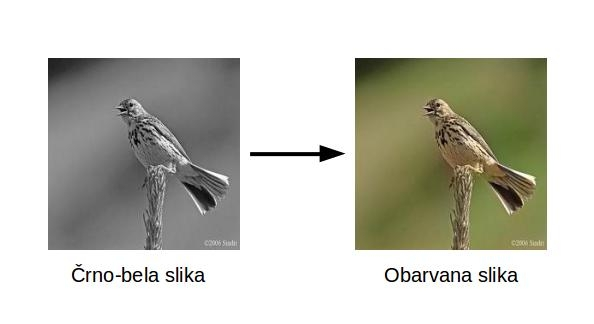
\includegraphics[width=12cm]{imcompare}
\end{center}
\caption{Pristop za vhod vzame črno-belo (sivinsko) sliko, preko nivojev nevronske mreže določi barvne komponente in na izhodu vrne obarvano sliko.}
\label{im:compare}
\end{figure}
 
Algoritmi za barvanje črno-belih slik dobijo kot vhod črno-belo sliko, ki ji dodajo barvo, kot je prikazano na sliki \ref{im:compare}. Pristopi za barvanje črno-belih slik se uporabljajo na več področjih: barvanje starih slik, barvanje črno-belih filmov in v umetnosti. V preteklosti so bili pristopi za barvanje slik pol-avtomatski \cite{levin2004colorization, huang2005adaptive, Koleini2010, shirley2001color, tai2005local}, danes pa jih zamenjujejo pristopi, ki obarvajo sliko popolnoma samostojno \cite{Cheng2015, Deshpande2015, Dahl, Zhang2016, larsson2016learning, Iizuka2016}. Zadnje raziskujemo v tem magistrskem delu.

\begin{figure}[hbt]
\begin{center}
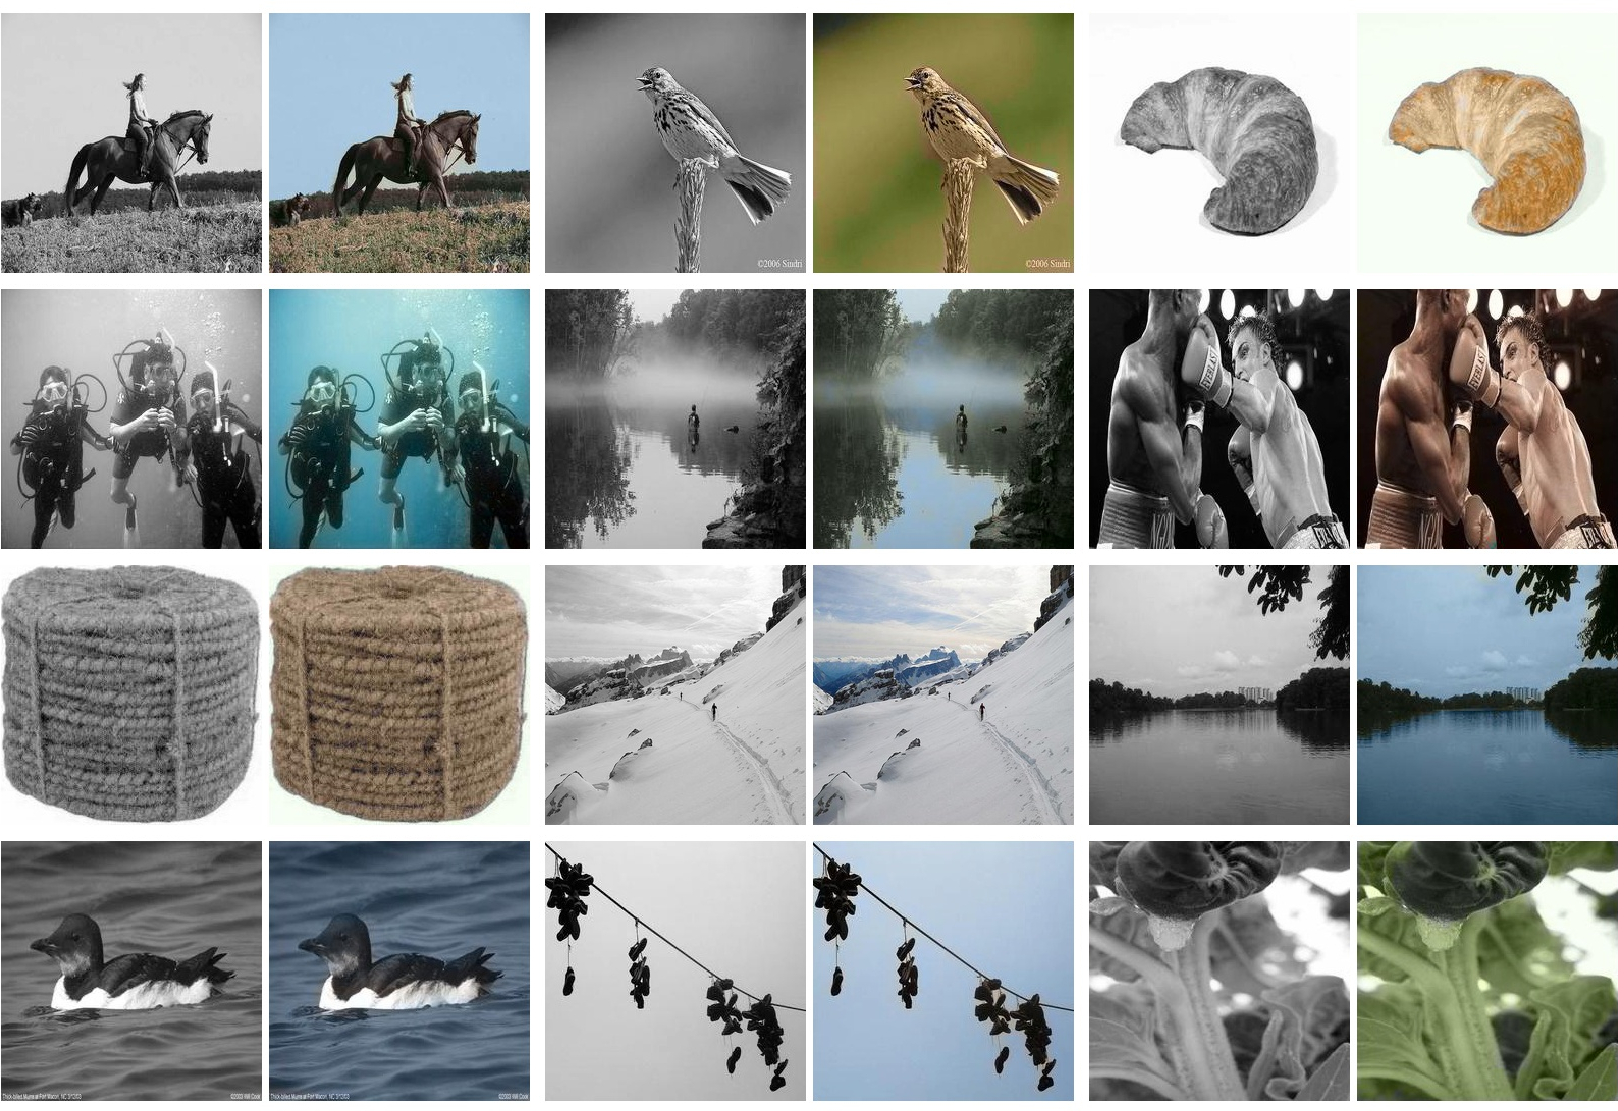
\includegraphics[width=13cm]{black-colored-comparison}
\end{center}
\caption{Primeri barvanja črno-belih slik. Barvanje je bilo izvedeno s pristopi, ki so bili razviti v okviru disertacije. Za vsako sliko je prikazana črno-bela slika, ki je vhod v algoritem in obarvana slika - izhod algoritma. }
\label{im:pari-cb-b}
\end{figure}

Za človeka je barvanje črno-belih slik, ki so prikazane na sliki \ref{im:pari-cb-b}, enostavna naloga. Z vsakdanjim opazovanjem sveta se je človek naučil, da je nebo modro z belimi oblaki, drevesa so zelena in cesta je siva. Za objekte, ki nimajo enolično določene barve, ljudje lahko uganemo kakšne barve naj bi bili. Pri tem opravilu je potrebno veliko razumevanja, saj iz sivinskih slik ni možno neposredno razbrati barv. Pri nastanku sivinskih slik se dve od treh dimenzij izgubita, saj je barvna slika zapisana z tremi barvnimi kanali v praktično kateremkoli barvnem prostoru, črno-bela pa le z enim barvnim kanalom, ki predstavlja sivino. Izgubi se kar dve tretjini informacij.

Problem postane bolj kompleksen, ko ga želimo rešiti na avtomatski način z računalnikom. Pri tem nam je v pomoč dejstvo, da je možno iz tekstur objektov le te prepoznati in jim na ta način določiti njihovo barvo \cite{Zhang2016}. Pri objektih, ki nimajo enolično določenih barv (na primer avtomobili, stavbe in knjige), je izziv mnogo težji. Pomaga nam dejstvo, da je naš cilj ohranjanje naravnega izgleda slike in ne reprodukcija originalnih barv. Nihče ne bo vedel, da je avtomobil, ki smo ga pobarvali modro, v resnici rdeče barve. 

Za barvanje slik smo implementirali pristope, ki uporabljajo nevronske mreže. Te delujejo podobno kot človeški možgani. Na začetku jih naučimo tako, da jim podamo čim več primerov barvanja slik, nevronska mreža pa naučeno znanje uporabi za barvanje slik.  
Mreži podamo sivinsko sliko, ki je kar $L*$ kanal barvnega prostora \textit{CIE Lab} \cite{Bansal}, vrne pa nam $a*$ in $b*$ kanal v istem barvnem prostoru. Barvni prostor podrobneje opišemo v razdelku \ref{ch:barvni-prostor}. Za učenje modela potrebujemo veliko črno-belih slik z referenčno barvno sliko, kar lahko z nekaj truda dobimo na spletu. Za učenje lahko vzamemo katerokoli sliko, jo pretvorimo v barvni prostor \textit{CIE L*a*b*}, kjer $L*$ kanal predstavlja sivinsko sliko. 

V nalogi rešujemo problem barvanja črno-belih slik z implementacijo različnih pristopov, ki vsi temeljijo na konceptu globokih nevronskih mrež. Rezultate smo ovrednotili s primerjavo med obarvano in originalno sliko. Rezultate lastnih algoritmov smo primerjali s tremi pristopi iz sorodnih del. Ker v naravi obstaja veliko objektov, ki nimajo enolične barve in je naš namen naravnost rezultatov, smo barvanje slik ocenjevali v spletni anketi in anketirance spraševali, katera obarvana slika je boljša.
V zadnjem delu disertacije smo pristope za barvanje slik prilagodili še za barvanje črno-belih filmov.

Na začetku si bomo v pregledu področja pogledali sorodna dela, nekaj ozadja o podatkih in globokih nevronskih mrežah. V tretjem poglavju so podrobno opisane arhitekture nevronskih mrež in predlagani različni pristopi za barvanje. V četrtem poglavju je opisano učenje nevronskih mrež, podatki in način evalvacije. V petem poglavju smo primerjali naše pristope s tistimi iz sorodnih del in si pogledali kateri pristopi in slike pri barvanju najbolj izstopajo. Preizkusili smo kateri pristop deluje najbolje na slikah večjih velikosti in naravnost barvanja preverili s spletno anketo. Za konec smo poskusili še z barvanjem videa.


%----------------------------------------------------------------
% Poglavje (Chapter) 2: Pregled področja
%----------------------------------------------------------------
\chapter{Pregled področja}
\label{ch:pregled}

Za barvanje črno-belih slik so bili razviti različni pristopi. Ti uporabljajo princip globokih nevronskih mrež. Pri pristopih je pomembna tudi predstavitev slikovnih podatkov.

\section[Predstavitev slikovnih podatkov in barvni prostori]{Predstavitev slikovnih podatkov in \\ barvni prostori}
\label{se:podatki}

Barvne slike, ki smo jih v disertaciji uporabili pri učenju, so shranjene v barvnem prostoru RGB \cite{Pm2013}. Kot je pokazano v \cite{Iizuka2016} se izkaže, da barvanje na osnovi prostora RGB daje slabše rezultate, saj prostor iz dveh razlogov ni primeren za učenje algoritmov za barvanje:

\begin{itemize}

\item \textbf{Sistem RGB se ne ujema dobro s človeško percepcijo barv}, saj so razdalje med enako sorodnimi barvami različne glede na odtenek \cite{Prangnell}. Na primer, če imamo dva para barv: temnejšo rdečo $(100, 0, 0)$ in svetlejšo rdečo $(208, 0, 0)$, ter temnejšo modro z vrednostmi $(0, 0, 100)$ in svetlejšo modro $(0, 0, 200)$, pri čemer sta barvi v obeh parih za človekov vizualni sistem enako podobni, sta razdalji med obema odtenkoma v RGB barvnem prostoru različni. Kot opazimo je razlika med obema modrima odtenkoma $100$, razlika med rdečima pa $108$. 

\item \textbf{Sistem RGB nima ločenega kanala za svetlost} \cite{Pm2013}. Glede na to, da modeli za barvanje napovedujejo le barvne elemente v sliki, svetlost pa privzamejo iz originalne slike, je najbolj priročno, če uporabljamo barvni prostor, ki ima ločen kanal za svetlost, saj je izhod metode združena komponenta za svetlost z barvnimi komponentami.

\end{itemize}

\subsection{Izbira primernega barvnega prostora}
\label{ch:barvni-prostor}

Na podlagi teh predpostavk je izbira prostorov omejena na prostore Lab \cite{Bansal}, YUV \cite{Jack2005} in HSL \cite{Pm2013}. Vsi našteti prostori vsebujejo ločen kanal za svetlost. Med njimi je Lab edini, kjer bližina barv v prostoru ustreza tudi percepcijski bližini.

Obstaja več implementacij barvnega prostora Lab, ki vse težijo k dobri aproksimaciji človeškega zaznavnega sistema. Enaka barva je v različnih implementacijah prostora Lab opisana z nekoliko drugačnimi vrednostmi, saj se je prostor razvijal skozi čas in postajal vedno bolj natančen. Trenutno se največ uporablja CIE L*a*b*, ki naj bi bil najboljša aproksimacija človeškega vizualnega sistema \cite{Prangnell}. Prostor ima tudi to prednost, da je neodvisen od naprave, ki je sliko zajela. 

Prostor CIE L*a*b* predstavi vse barve, ki jih je možno zaznati s tremi barvnimi kanali. Zaloga vrednosti $L*$ predstavlja svetlost, $a*$ se razširja od zelene proti rdeči in $b*$ od modre proti rumeni barvi. Prostor je grafično prikazan na sliki \ref{im:lab}. Zaloga vrednosti $L*$ se raztezajo od $0$, ki predstavlja črno barvo, do $100$, ki predstavlja belo barvo \cite{Weatherall1992}. Komponenti $a*$ in $b*$ načeloma nista omejeni, vendar sta v implementacijah omejeni na vrednosti v intervalu $[-128, 127]$, kar je možno predstaviti z osem bitnim celim številom\footnote{\url{https://www.freiefarbe.de/en/grenzen-des-cielab-farbraums/}}. Ker zaradi pretvorbe iz barvnega prostora RGB vrednosti komponent $a*$ in $b*$ višje od $100$ ali nižje $-100$ redko dosežemo, smo opazili, da nekatere implementacije omejijo zalogo vrednosti barvnih komponent na interval $[-100, 100]$. Za pomoč pri implementaciji nevronske mreže, smo sami preizkusili, kakšen je dejanski interval barv pretvorjenih iz barvnega prostora RGB. Intervale si lahko pogledate v tabeli \ref{tab:rgbcie}.

\begin{figure}[hbt]
\begin{center}
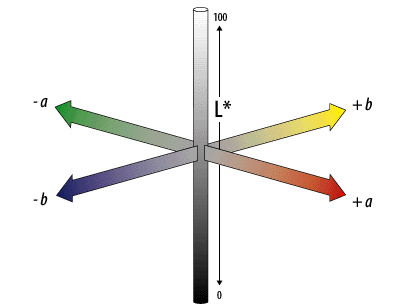
\includegraphics[width=6cm]{cielab}
\end{center}
\caption{Slika prikazuje kanale barvnega prostora CIE L*a*b*. $L*$ predstavlja svetlost, $a*$ se razteza od zelene barve v najbolj negativni točki proti rdeči barvi, $b*$ pa se razteza od modre proti rumeni. Nasprotujoče barve na kanalih $a*$ in $b*$ se nikoli ne kombinirajo v odtenek. Iz: Adobe, Technical Guid, CIELAB\protect\footnotemark{} (dostopano: 24. junij 2017)}
\label{im:lab}
\end{figure}

\footnotetext{\url{http://dba.med.sc.edu/price/irf/Adobe_tg/models/cielab.html}}

\begin{table}[htb]
\caption{Največje in najmanjše vrednosti posamezne komponente barvnega prostora CIE L*a*b* pri pretvorbi  barv iz barvnega prostora RGB. Pretvorba je bila narejena z uporabo osvetlitve $D65$, ki določa temperaturo bele točke. Izkaže se, da je večina vrednosti komponent $a*b*$ znotraj intervala $[-100, 100]$. }
\begin{center}
    \begin{tabular}{lccc}
    	\hline
        Kanal & Najmanjša vrednost & Največja vrednost \\
        \hline
        L* & 0 & 100 \\
        a* & -86,185 & 98,254 \\
        b* & -107,863 & 94,482 \\
        \hline
    \end{tabular}
\end{center}
\label{tab:rgbcie}
\end{table}

\subsection{Pretvarjanje med barvnim prostorom RGB in CIE L*a*b*}

Za pretvorbo med prostoroma ni enostavne enačbe, saj je barvni prostor RGB odvisen od naprave, ki sliko zajame, CIE L*a*b* pa je neodvisen. V našem primeru imamo slike že zapisane v standardnem RGB ali sRGB barvnem prostru, ki je neodvisen od naprave. V ta prostor je bila slika pretvorjena že ob zajemu. Pretvorba se zato zgodi v dveh korakih \cite{Connolly1997}: 

\begin{enumerate}

\item \textbf{Pretvorba v barvni prostor CIE 1931} \cite{Ohta2005} ali drugače imenovan barvni prostor CIE XYZ. Ta pretvorba se izvede s pomočjo linearne pretvorbe - množenje z matriko. Matrika je odvisna od izbire referenčne bele barve \cite{Ohta2005}. Običajno se izbere referenčno temperaturo bele točke \textit{D65}, ki je tudi standardizirana\footnotemark{}.

\footnotetext{Zapis na uradni strani komisije International Commision on Illumination (krajše CIE), ki je postavila standard, pravi, da se kot standardno uporablja referenčno temperaturo bele točke D65: \url{http://cie.co.at/index.php?i_ca_id=484}}

\item \textbf{Pretvorba iz CIE XYZ v L*a*b*} se izvede z uporabo transformacijskih enačb opisanih v članku XYZ to LAB\footnote{\url{http://www.brucelindbloom.com/index.html?Eqn\_XYZ\_to\_Lab.html}}.  

\end{enumerate}

Pretvorbo med barvnima prostoroma sRGB in CIE L*a*b* demonstrira sledeča implementacija v Pythonu. 

\inputminted{python}{rgb2lab.py}

\section{Globoke nevronske mreže}
\label{se:globoke}

Globoke nevronske mreže so algoritmi, ki so zgrajeni na podlagi opazovanja strukture možganov. Uporabljajo se za klasifikacijo, regresijo, gručenje in napovedovalno analizo. Pogosto se uporabljajo na področju analize slik, kjer je zelo pomembno prepoznavanje objektov in obrazov, razvrščanje slik v skupine glede na podobnost, prepoznavanje gest in barvanje slik\footnote{\label{fndeep}https://deeplearning4j.org/neuralnet-overview}.

Nevronska mreža je v osnovi funkcija $f(\vec{x})$, ki preslika vhod $\vec{x}$ v izhod $\hat{y}$. Med postopkom učenja je ta funkcija optimizirana tako, da najde najboljšo aproksimacijo dejanskih vrednosti $\vec{y}$, ki so za učne podatke znani\footnoteref{fndeep}. Nevronska mreža je struktura, ki je sestavljena iz več nivojev. Nivoje si lahko predstavljamo kot vrsto vozlišč, ki se odzovejo v primeru dovolj visokih signalov na vhodu. Primer strukture vozlišča in nivojev je predstavljena na sliki \ref{im:nn-structure}. Vozlišče pomnoži vhodne vrednosti s trenutnimi vrednostmi uteži, doda še pristranskost (ang. {\em bias}), vrednosti sešteje in moč aktivacije izračuna s pomočjo tako imenovane aktivacijske funkcije, ki tvori izhod vozlišča. Aktivacijski funkciji rečemo tudi nelinearnost, saj poskrbi za to, da nevronska mreža ni le linearna funkcija. Tipični primeri takih funkcij so sigmoidna funkcija, tanh, ReLU, leaky ReLU in maxout \cite{Karpathy2016a}. Uteži se skozi postopek učenja spreminjajo in s tem določajo aktivacijo vozlišča.

\begin{figure}[htb]
\begin{center}
\centering
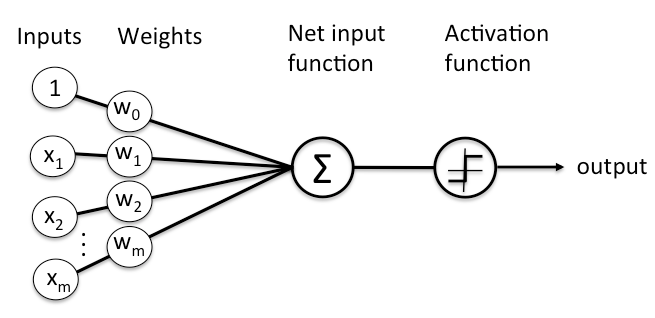
\includegraphics[width=7cm]{node_structure}
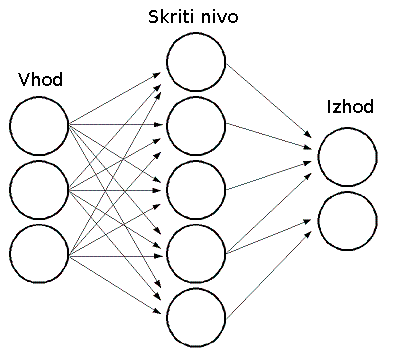
\includegraphics[width=4cm]{nn_structure}
\end{center}
\caption{Leva slika prikazuje zgradbo enega vozlišča nevronske mreže. Vhod je lahko izhod prejšnjega nivoja ali predstavlja vhodne podatke, ki se potem pomnožijo z utežmi in seštejejo. Desna slika prikazuje zgradbo večnivojske nevronske mreže. V našem primeru ima ta en vhodni nivo, en skriti nivo in izhodni nivo. Iz: Introduction to Deep Neural Networks\protect\footnotemark{} in Neural Networks\protect\footnotemark{} (dostopano: 21. junij 2017).}
\label{im:nn-structure}
\end{figure}

\footnotetext[6]{\url{https://deeplearning4j.org/neuralnet-overview}}
\footnotetext{\url{http://docs.opencv.org/2.4/modules/ml/doc/neural\_networks.html}}


Nivojem v nevronskih mrežah, ki se nahajajo med vhodnim in izhodnim nivojem, pravimo skriti nivoji (ang. {\em hidden layers}) \cite{Karpathy2016a}. Tradicionalni algoritmi na področju strojnega učenja so sestavljeni iz vhodnega, izhodnega nivoja in enega skritega nivoja, globoka nevronska mreža (ang. {\em deep neural network}) pa ima vsaj dva skrita nivoja \cite{collobert2008unified}, pri večini praktičnih implementacij pa jih je mnogo več. Vsak nivo globoke nevronske mreže prepozna določene lastnosti vhodnih podatkov. Nivoji, ki se nahajajo globje, lahko prepoznajo bolj kompleksne lastnosti podatkov, saj na vhodu dobijo značilke, ki še dodatno opisujejo vhodne podatke. 

Da nevronska mreža daje zadovoljive rezultate je potrebno utežem do\-lo\-či\-ti prave vrednosti. To naredimo z učenjem. Vsaka nevronska mreža ima cenilno funkcijo (ang. {\em loss function}), ki pove, kako dobre rezultate daje nevronska mreža na testnih podatkih. V postopku učenja je cilj zmanjšati vrednost cenilne funkcije z enim od algoritmov optimizacije. Tipične cenilne funkcije so: cenilna funkcija večrazredne metode podpornih vektorjev (ang. {\em Multiclass Support Vector Machine loss}), križna entropija, L2 norma (povprečna kvadratna napaka) in L1 norma \cite{Karpathy2016set}. 

\subsection{Konvolucijske nevronske mreže}

Ker bi bilo na primeru slik pri uporabi klasičnih nevronskih mrež hitro preveč parametrov, kar bi poleg podaljšanja časa učenja povzročilo tudi prekomerno prilagajanje (ang. {\em overfitting}) in pomanjkanje pomnilnika, uporabljamo konvolucijske nevronske mreže. Te so tako kot običajne nevronske mreže estavljene iz nevronov, ki imajo svoje uteži in pristranskost. Ti parametri so učljivi. Operacije znotraj nevrona so podobne tistim pri običajnih nevronskih mrežah, le da so prilagojene pričakovanim vhodnim podatkom - slikam. Vhod v vsak nivo nevronske mreže je torej tenzor $X$ z obliko $vi\check{s}ina \times \check{s}irina \times globina$, kjer globina pomeni število barvnih kanalov slike \cite{Karpathy2016}. Konvolucijske nevronske mreže so v osnovi sestavljene iz treh vrst nivojev:

\begin{itemize}

\item \textbf{Konvolucijski nivo} je glavni gradnik konvolucijske nevronske mreže. Parametri tega nivoja so sestavljeni iz majhnih konvolucijskih jeder, ki pokrivajo majhno polje slike. Več takih jeder pa pokrivajo celotni nivo v globino, tako si lahko eno jedro predstavljamo kot utež pri skritih nivojih v običajni nevronski mreži, ki zraven izvaja še konvolucijo. Med prehodom po nevronski mreži izvedemo konvolucijo po celotni višini in širini vhodnega tenzorja, po globini pa se izhode teh konvolucij sešteje enako kot pri običajni nevronski mreži. Izhod konvolucije z enim setom jeder je dvodimenzionalna matrika \cite{lecun1995convolutional}. Na sliki \ref{im:convolution_ex} je shema, ki prikazuje delovanje posamezne konvolucije.

\begin{figure}[hbt]
\begin{center}
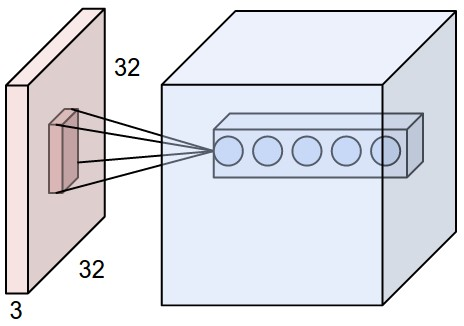
\includegraphics[width=8cm]{depthcol}
\end{center}
\caption{Primer, ki prikazuje potek konvolucije. Vhodni tenzor je po celotni višini in širini konvuliran s setom konvolucijskih jeder. Izhod ene operacije je enodimenzionalni tenzor, v tem primeru ima ta pet elementov in vpliva le na del izhodnega tenzorja. Skupek vseh konovlucij tvori celoten izhodni tenzor. Vir slike: Karpathy \cite{Karpathy2016}}.
\label{im:convolution_ex}
\end{figure}

\item \textbf{Nivo združevanja (ang. {\em pooling layer})} je namenjen podvzorčenju (ang. {\em downsampling}) tenzorja. To izvede tako, da združi več izhodov iz nevronov nekega nivoja v posamezen nevron v naslednjem nivoju. Za združevanje obstaja več strategij. Najbolj pogosto je maksimalno združevanje (ang. {\em max pooling}), poznamo pa še povprečno združevanje (ang. {\em average pooling}). S združevanjem zmanjšamo prostorsko dimenzijo tenzorja in s tem število parametrov, kar vpliva na zmanjšanje računske zahtevnosti in prekomernega prilagajanja. Deluje na principu, da je točna lokacija značilke manj pomembna kot približna lokacija glede na ostale značilke. \cite{Krizhevsky2012}. 

\item \textbf{Polnopovezni nivo} je nivo enak skritim nivojem pri klasični nevronski mreži. Večinoma se uporabi za zadnjih nekaj nivojev pri konvolucijski nevronski mreži, če je to primerno za dano nalogo.

\end{itemize}

\subsection{Primer konvolucijske nevronske mreže}
\label{ch:cov_nev_net}

Za primer konvolucijske nevronske mreže bomo predstavili poenostavljeno mrežo za prepoznavanje objektov v sliki. Ta naloga je namreč postala šolski primer uporabe konvolucijskih nevronskih mrež. 

Odločili smo se implementirati mrežo, ki na vhodu prejme sliko velikosti $h \times w$ slikovnih točk in ima tri barvne kanale prostora RGB. Mreža na izhodu vsako sliko klasificira v enega od razredov. Za demonstracijo smo se odločili, da bomo slike klasificirali v enega od desetih razredov, čeprav večina ostalih implementacij slike razvršča v mnogo več razredov. Primeri razredov so na primer živali, drevesa, zgradbe, morje in ljudje in so odvisne od podatkovne zbirke s katero učimo mrežo.

Mreža, ki jo uporabljamo za to nalogo, je shematsko prikazana na sliki \ref{im:vgg-like}. Na začetku ima mreža dva konvolucijska nivoja, nato sledi nivo maksimalnega združevanja, ki zmanjša prostorsko dimenzijo tenzorja. Sledita še dve konvoluciji in še eno maksimalno združevanje. Takoj za tem se tenzor splošči v enodimenzionalni tenzor in gre preko dveh polnopovezanih nivojev. Prvi velikost enodimenzionalnega tenzorja zmanjša na velikost $256$ drugi pa na velikost $10$. Vsaka vrednost v zadnjem tenzorju predstavlja verjetnost za pripadnost objekta na sliki določenemu razredu. Razred z največjo verjetnostjo predstavlja objekt na sliki. 

\begin{figure}[htb]
\begin{center}
\centering
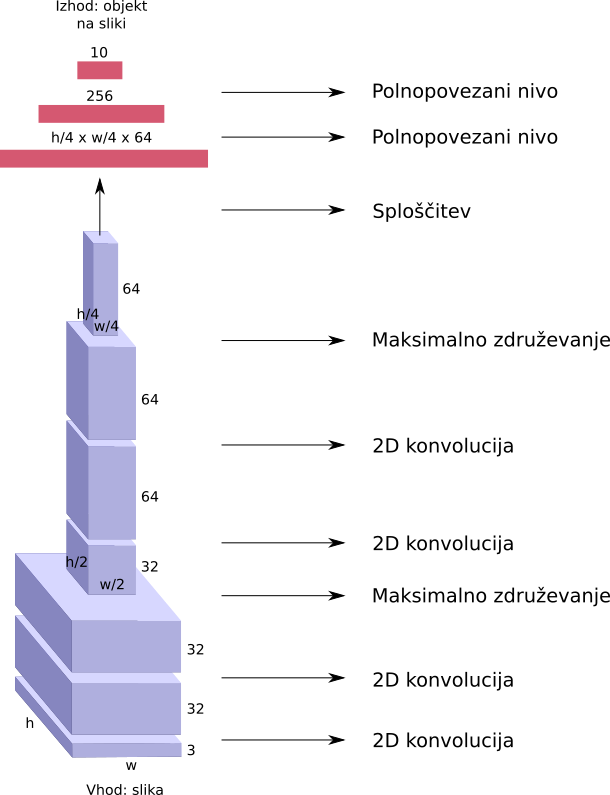
\includegraphics[width=7cm]{vgg_like_arh}
\end{center}
\caption{Shematski prikaz poenostavljene nevronske mreže za prepoznavanje objektov na sliki. Na levi strani je prikazano spreminjanje velikosti tenzorjev ob prehodu skozi nevronsko mrežo, na desni pa so označeni nivoji mreže.}
\label{im:vgg-like}
\end{figure}

Vsak nivo ima tudi svojo aktivacijsko funkcijo. Pri vseh nivojih uporabljamo funkcijo ReLU, razen pri zadnjem polnopovezanem, kjer je aktivacijska funkcija softmax. Glede na to, da gre za klasifikacijski problem za cenilno funkcijo, uporabljamo križno entropijo. Primer implementacije te nevronske mreže v vmesniku Keras je predstavljen v poglavju \ref{ch:keras}.


\subsection{Konvolucijske nevronske mreže v Kerasu}
\label{ch:keras}

Keras \cite{chollet2015keras} je visokonivjski aplikacijski programski vmesnik za nevronske mreže. Vmesnik lahko teče na zaledju Tensoflow \cite{tensorflow2015-whitepaper}, Theano \cite{2016arXiv160502688short} ali CNTK \cite{Seide:2016:CMO:2939672.2945397}. V našem primeru smo izbrali Tensorflow.
Razlog za izbiro vmesnika Keras je, da je visokonivojski in zaradi tega uporabniku prijazen, narejen je v programskem jeziku Python\footnote{\url{https://www.python.org/}}, ki nam je najbolje poznan in je zelo modularen, nevronska mreža je predstavljena kot sekvenca ali graf, ki jo je enostavno dopolniti ali spremeniti.

V vmesniku Keras smo za demonstracijo implementirali konvolucijsko nevronsko mrežo iz poglavja \ref{ch:cov_nev_net}..

\inputminted{python}{vvg_like.py}

% podatki
Kot je opazno iz prvega dela implementacije, so podatki, ki smo jih pripravili, naključno generirani. Ti podatki nam ne zagotavljajo smiselnega učenja, iz njih pa lepo vidimo strukturo podatkov. 
Pri podatkih predpona $x$ običajno označuje, da gre za vhodne podatke v mrežo, $y$ označuje prave vrednosti oziroma pričakovane izhode iz mreže. Običajno razlikujemo med tremi vrstami podatkov. Učni podatki ($x_training$, $y_training$) so tisti, ki jih uporabimo zgolj za učenje mreže, validacijski podatki ($x_validation$, $y_validation$) so tisti, ki imajo tako kot učni podatki zraven prisotne prave vrednosti in služijo preverjanju natančnosti mreže. Testni podatki ($x_test$) so tisti, ki jih na koncu uporabimo za prikaz rezultatov mreže. Velikokrat testni podatki nimajo prisotnih pravih vrednosti. Na primer pri raznih tekmovanjih na področju strojnega učenja tekmovalec dobi le vhodne podatke, napovedi pa odda za kasnejše vrednotenje, pri čemer ne vidi pravilnih napovedi.

% nekaj o zgradbi
Mreža ima sekvenčno zgradbo, konvolucijski nivoji uporabljajo jedro velikosti $3 \times 3$, pri maksimalnem združevanju (MaxPooling) uporabljamo velikost združevanja $2 \times 2$, kar pomeni, da se velikost tenzorja po višini in širini zmanjša za faktor polovico. V implementaciji se uporabljajo tudi nivoji za opustitev nevronov (Dropout), ki v vsakem koraku učenja izločijo določen delež vozlišč. Ta vozlišča s tem ne vplivajo na rezultat napovedi in se v tistem koraku tudi ne učijo. S tem zmanjšajo prekomerno prilagajanje (ang. {\em overfitting}).

% učenje
Pri učenju smo uporabljali optimizator Adam \cite{DBLP:journals/corr/KingmaB14}. Optimizator je algoritem, ki določa strategijo spreminjanja uteži in s tem zmanjšuje vrednost cenilne funkcije. Najbolj enostavni optimizator je gradientni sestop, ki spreminja uteži v smeri najhitrejšega zmanjševanja napake, vendar to ni vedno dovolj učinkovito, zato so bili razviti novi algoritmi. Najbolj se uporabljajo: SGD, Adagrad, RMSprop in Adam \cite{Karpathy2016learning}. 

Kot lahko opazimo ob pogledu na funkcijo $fit$ vidimo, da je parameter $epochs$ nastavljen na fiksno število korakov. V tem primeru mrežo učimo z $10$ prehodi skozi vse podatke. Običajno se trajanje učenja določi s spremljanjem obnašanja validacijske napake. Z učenjem končamo, ko se validacijska napaka neha zmanjševati. Takrat pravimo, da je algoritem skonvergiral k najmanjši napaki. Če bi z učenjem nadaljevali se začne mreža prekomerno prilagajati učnim podatkom, kar v večini primerov pomeni, da se slabše odreže na validacijskih in kasneje testnih podatkih.

\subsection{Cenilne funkcije}
\label{ch:cenilne}

Pri pristopih opisanih v tem delu uporabljamo tri cenilne funkcije. Pri regresijskih pristopih se je za dobro izkazala cenilna funkcija povprečna kvadratna napaka (ang. {\em mean squared error}), ki jo označimo z MSE in je predstavljena z enačbo \ref{eq:mse}. V enačbi $Y$ predstavlja originalno sliko, $\hat{Y}$ pa obarvano sliko s strani mreže. Spremenljivka $h$ je višina slike, $w$ je širina slike in $c$ je število kanalov. MSE smo računali le na komponentah $a*$ in $b*$, tako da je $c=2$.  

\begin{equation}
\textrm{MSE}(\hat{Y}, Y) = \frac{1}{hwc} \sum_{h, w, c} (Y_{h,w,c} -  \hat{Y}_{h,w,c})^2
\label{eq:mse}
\end{equation}

Pri enem od klasifikacijskih pristopov smo uporabili cenilno funkcijo divergenca Kull\-back-Leibler \cite{joyce2011kullback}, ki jo označujemo z oznako $\textrm{D}_{KL}$. V našem primeru smo izvedli divergenco Kullback-Leibler na posamezni slikovni točki in jo povprečili preko celote slike kot prikazuje enačba \ref{eq:kld}. V enačbi $Z$ predstavlja originalno sliko, $\hat{Z}$ pa obarvano sliko s strani mreže, obe sta pretvorjeni v vektorje s $400$ razredi, ki predstavljajo barve. Spremenljivka $h$ je višina slike, $w$ je širina slike, oznaka $c$ v tem primeru predstavlja število razredov, v katere mreža klasificira barve, zato je $c = 400$. 

\begin{equation}
\textrm{D}_{KL}(Z || \hat{Z}) = \frac{1}{hw} \sum_{h, w} \sum_c Y_{h, w, c} \log \frac{Z_{h, w, c}}{\hat{Z}_{h, w, c}}
\label{eq:kld}
\end{equation}

Zadnja cenilna funkcija je križna entropija (ang. {\em cross entropy}) \cite{Mannor2005} in jo bomo krajše označili z $H$. Zaradi različnih implementacij uporabljamo dve različici križne entropije. Prva je brez uteži in je predstavljana v enačbi \ref{eq:ce}, kjer so oznake enake oznakam iz enačbe \ref{eq:kld}. Križna entropija se računa na razredih napovedanih s strani mreže.

\begin{equation}
\textrm{H}(\hat{Z}, Z) = \sum_{h, w, c} Z_{h, w, c} \log \hat{Z}_{h, w, c}
\label{eq:ce}
\end{equation}

Druga različica križne entropije uporablja uteži, ki predstavljajo povprečno pogostost pojavitve posamezne barve v slikah. Pogostost je bila izračunana na množici $100 000$ naključnih slik izbranih iz zbirke ImageNet. Princip uteži v cenilni funkciji da večji pomen tistim točkam, kjer se v originalni sliki pojavijo močnejše barve. S tem želimo vzpodbuditi mrežo, da bo večkrat obarvala z močnejšimi barvami. Pri ostalih pristopih je namreč problem, da barve velikokrat niso tako močne in živahne, kot bi lahko bile. Križno entropijo z utežmi označimo s $Hw$ in jo definiramo z enačbo \ref{eq:cew}, kjer $v(\cdot)$ predstavlja utež za barvo v slikovni točki na koordinatah $(h, w)$. 

\begin{equation}
\textrm{Hw}(\hat{Z}, Z) = \sum_{h, w} v(Z_{h, w}) \sum_{c} Z_{h, w, c} \log \hat{Z}_{h, w, c}
\label{eq:cew}
\end{equation}

\section[Metode za barvanje črno-belih slik]{Metode za barvanje črno-belih slik}

Pristope za barvanje črno-belih slik lahko delimo v dve večji skupini. Prva zahteva interakcijo uporabnika med postopkom barvanja, ki se je več uporabljala v preteklosti, pri drugi pa barvanje poteka popolnoma avtomatsko.

\subsection{Pristopi z interakcijo uporabnika}

To skupino pristopov delimo na tehnike, ki temeljijo na uporabnikovem barvanju manjših delov slik (ang. {\em scribble based}) \cite{levin2004colorization, huang2005adaptive} in tiste, ki temeljijo na primerih podobno obarvanih slik (ang. {\em example based}) \cite{Koleini2010, shirley2001color, tai2005local}. 

Pri prvih uporabnik določi barvo nekaj točk na sliki, te pa algoritem avtomatsko razširi preko cele slike. Kvaliteta barvanja je odvisna od zahtevnosti slike in števila točk, ki jih je uporabnik označil.
Pri barvanju na primerih uporabnik izbere referenčno sliko podobno tisti, ki jo želimo obarvati, algoritem pa lastnosti izbrane slike razširi na drugo sliko ali množico slik. Kvaliteta barvanja je odvisna od podobnosti referenčne slike s sliko, ki jo barvamo. 

Prednost tehnike barvanja, ki temelji na barvanju manjših delov je, da je barvanje lahko zelo natančno in naravno, vendar mora uporabnik za dovolj veliko natančnost označiti veliko točk na sliki. V nasprotnem primeru je lahko barvanje tudi zelo nenatančno. 
Prednost tehnike barvanja s primeri pa je njena hitrost in avtomatičnost po tem, ko imamo izbrano referenčno sliko, vendar je velikokrat problem dobiti dobro referenčno sliko.
Zaradi teh lastnosti se tehnika barvanja s primeri uporablja za barvanje videa, saj je v tem primeru potrebno ročno pobarvati na primer vsako stoto sliko, na ostale pa algoritem sam razširi lastnosti ročno barvane slike. 
Ta tehnika je večinoma zelo natančna, saj se slike, ki so v videu blizu običajno zelo malo razlikujejo, vendar še vedno vključuje veliko ročnega dela.

\subsection{Popolnoma avtomatski pristopi}

V magistrskem delu se osredotočamo na avtomatske pristope barvanja. Ti pristopi samostojno brez uporabnikovega posredovanja obarvajo celotno sliko. Prva dva pristopa, ki sta bila predlagana na tem področju, temeljita na značilkah (ang. {\em features}) slik. Tukaj gre predvsem za značilke, ki opisujejo intenziteto posamezne barve in značilke, ki opisujejo robove v sliki. Prvi pristop uporablja za barvanje nevronsko mrežo \cite{Cheng2015}, ki vsebuje zgolj polnopovezane nivoje, druga pa za barvanje uporabi metodo naključnih gozdov (ang. {\em random forest}) \cite{Deshpande2015}. 

Novejši pristopi barvanja črnobelih slik tipično temeljijo na konvolucijskih nevronskih mrežah, ki v vsakem nivoju same odkrijejo značilke, ki so pomembne za čimbolj kvalitetno barvanje. Prva tovrstna rešitev \cite{Dahl} gradi mrežo na podlagi  že zgrajene šestnajst-nivojske mreže VGG-16, ki so jo razvili na univerzi v Oxfordu \cite{Simonyan2014} in je namenjena prepoznavanju objektov v sliki. Rešitev uporablja evklidsko cenilno funkcijo in barvni prostor YUV \cite{Jack2005}. Slabost te rešitve je, da izhodne barvne slike niso dovolj nasičene in poudarjajo rjave odtenke. 

V zadnjem času predlagane rešitve popravijo problem nenasičenosti kar z uporabo softmax funkcije v zadnjem nivoju nevronske mreže. Problem barvanja na ta način spremenijo iz regresijskega v klasifikacijskega.  
Zang in sod. \cite{Zhang2016} uporabijo konvolucijsko nevronsko mrežo z več nivoji in aktivacijskimi funkcijami ReLU. Uporabljajo barvni prostor L*a*b*. Arhitektura je predstavljena na sliki \ref{im:zgang-arh}. Posebnost te mreže je cenilna funkcija. Uporablja križno entropijo opisno z enačbo \ref{eq:cross_ent_weights}, ki je v tem primeru izvedena na primerjavi barv vsake slikovne točke glede na barvni prostor, ki je kvantiziran. $Z$ predstavlja barve originalne slike, ki so zapisane kot vektorji z vrednostjo ena, za razred v katerega barva spada, $\hat{Z}$ je ocenjena barva.  Napake so pomnožene z utežjo, ki določa pogostost barve. Redkeje uporabljene barve so obtežene tako, da prispevajo večji delež k cenilni funkciji. S tem so avtorji izboljšali rezultate tako, da se bolj pogosto pojavljajo tudi močnejši odtenki, torej tisti z višjimi vrednostmi v barvnem prostoru \textit{a*b*}, ki so bili prej redkeje zastopani zaradi bolj pogostega pojavljanja nežnejših barv v slikah. To so barve bližje vrednostim $(0, 0)$ v \textit{a*b*} prostoru. V enačbi \ref{eq:cross_ent_weights} za obteževanje vrednosti poskrbi funkcija $v(\dot)$.
Pogostost je bila izračunana z analizo vseh slik v podatkovni zbirki Imagenet \cite{ILSVRC15}. 

\begin{equation}
H(\hat{Z}, Z) = - \sum_{h, w} v(Z_{h, w}) \sum_c Z_{h, w, c} \log (\hat{Z}_{h, w, c}) 
\label{eq:cross_ent_weights}
\end{equation}

\begin{figure}[htb]
\begin{center}
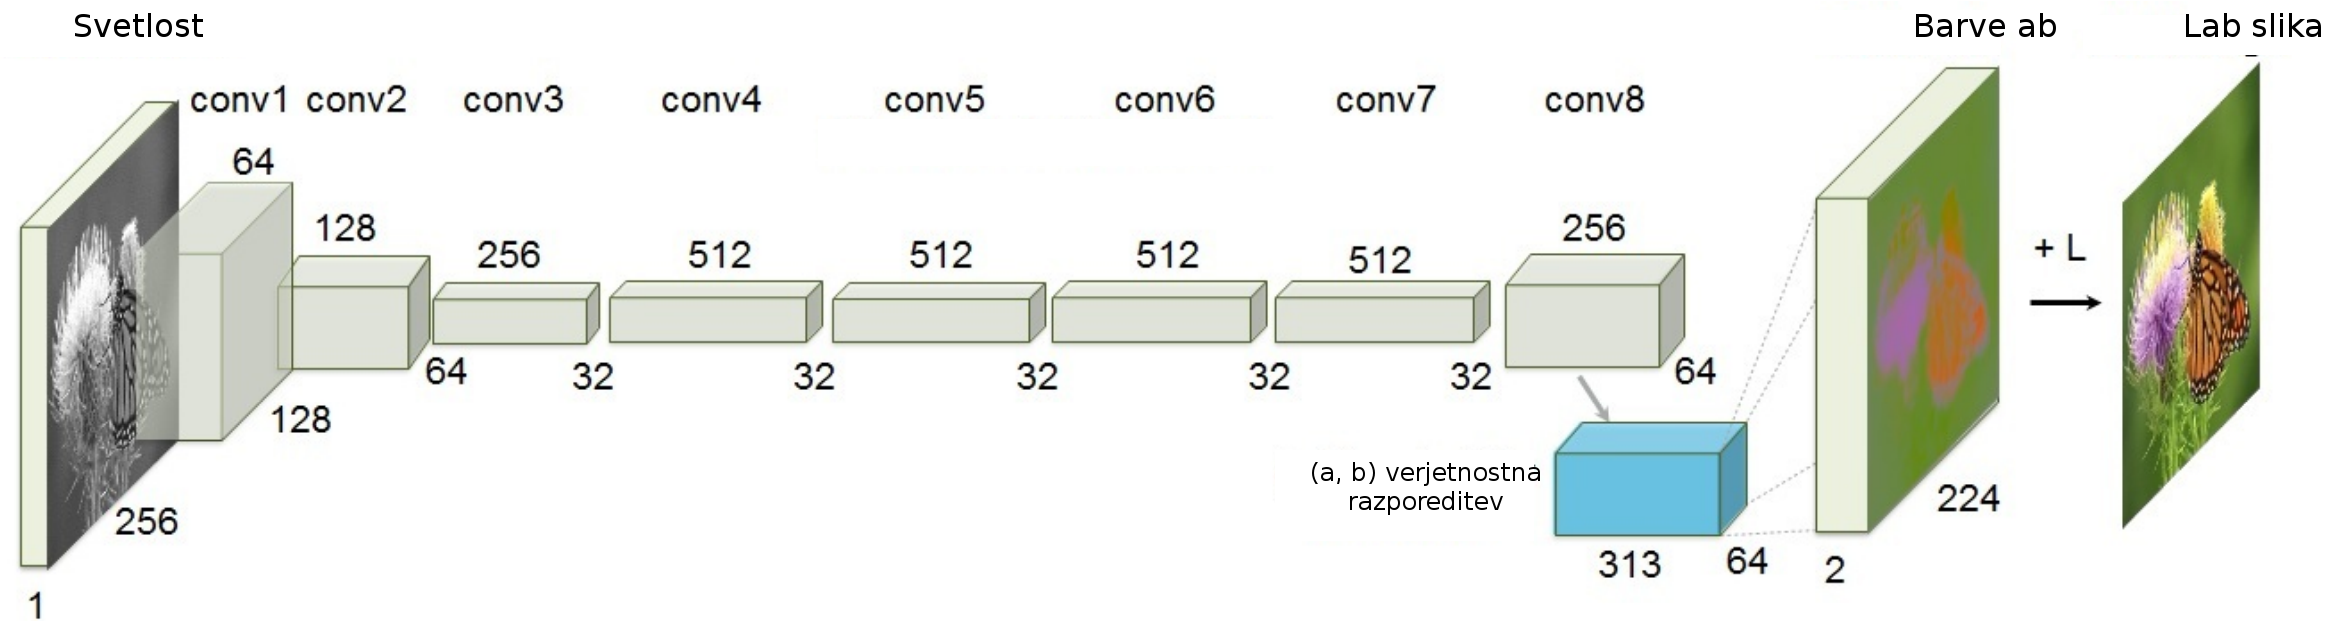
\includegraphics[width=12cm]{zhang_arh}
\end{center}
\caption{Slika prikazuje arhitekturo mreže Zang in sod. \cite{Zhang2016}. Na vhodu mreža dobi črno-belo sliko, nato sledi več konvolucijskih blokov. Vsak od blokov vsebuje dve ali tri konvolucije. Vsaki konvoluciji sledi normalizacija serije (ang. {\em bacth normalization}) in aktivacijska funkcija ReLU. Modri blok predstavlja napovedi barve v obliki verjetnosti za vsak razred, ki predstavlja množico odtenkov. Te vrednosti se na koncu pretvorijo v barvne vrednosti $a*b*$ in združijo s črno-belo sliko, da dobimo obarvano sliko. Vir slike: Zang in sod. \cite{Zhang2016}. }
\label{im:zgang-arh}
\end{figure}
 
Larsson in sod. \cite{larsson2016learning} za osnovo uporabijo mrežo VGG-16, iz katere vzamejo tenzorje vsakega nivoja, ki jim povečajo prostorsko dimenzijo, tako da se ujemajo in združijo v enotno matriko. Sledi še en polno-povezan nivo. Rezultat klasifikacije je histogram z verjetnostmi posameznega odtenka za vsako točko na sliki. Arhitektura mreže je predstavljena na sliki \ref{im:larsson-arh}. Uporabljajo barvni prostor HSV, ki ga prilagodijo zaradi nestabilnosti v delu prostora v komponente: odtenek označen z $H$, barvna nasičenost označena z $C$ in svetlost $L$. Cenilna funkcija, ki jo uporabljajo, je divergenca Kullback-Leibler prikazana v enačbi \ref{eq:kl_div}, ki primerja izhodni histogram z originalno sliko pretvorjeno v histogram po zgoraj opisanih komponentah. V enačbi \ref{eq:kl_div}  $Z$ predstavlja originalno sliko spremenjeno v histogram vrednosti za vsako od komponent $H$ in $C$, $\hat{Z}$ predstavlja ocenjeno barvo. Utež $\lambda$ pove koliko k napaki prispeva vsaka od komponent $C$ in $H$ in so jo avtorji nastavili na vrednost $\lambda = 5$.

\begin{equation}
\begin{gathered}
L(\hat{Z}, Z) = \sum_{h, w} \left(D_{KL}(Z_{h, w, C} ||  \hat{Z}_{h, w, C}) + \lambda D_{KL}(Z_{h, w, H} || \hat{Z}_{h, w, H})\right) \\ 
D_{KL}(z ||  \hat{z}) = \sum_{i} z_{i} \log \frac{z_{i}}{\hat{z}_{i}}
\end{gathered}
\label{eq:kl_div}
\end{equation}

\begin{figure}[htb]
\begin{center}
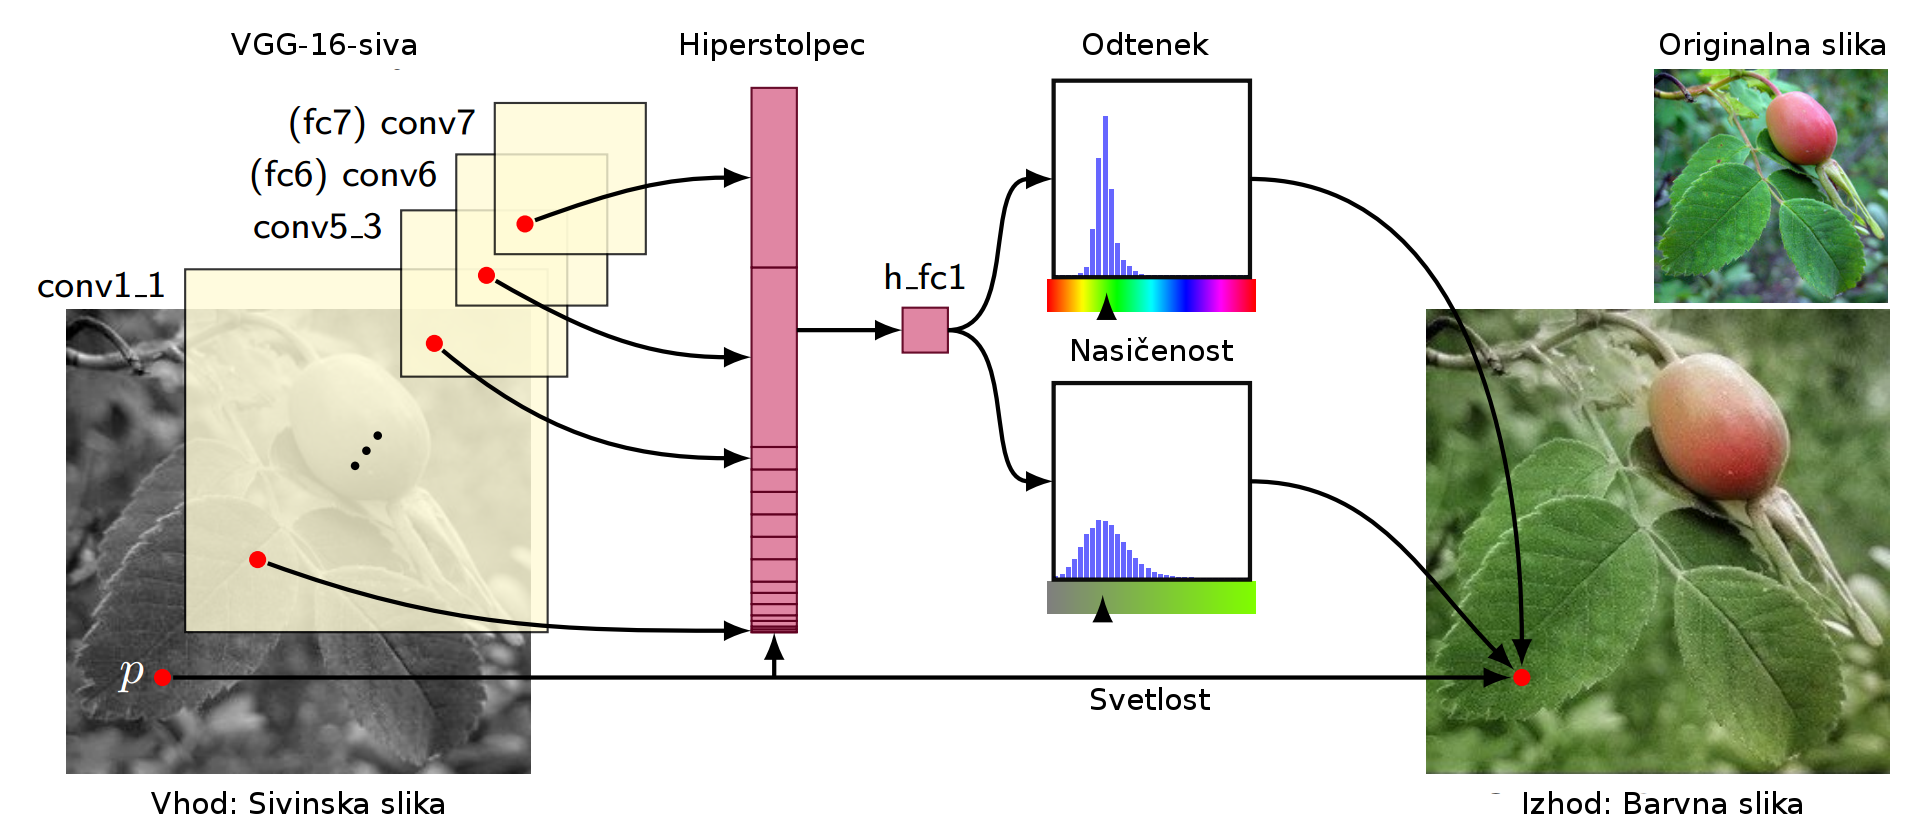
\includegraphics[width=11cm]{larson_arh}
\end{center}
\caption{Slika prikazuje arhitekturo mreže Larsson in sod. \cite{larsson2016learning}. Mreži VGG-16 je podana črno-belo slika, nato se iz omenjene mreže vzame izhode vseh konvolucij in polnopovezanih nivojev, jih nadvzorči na velikost osnovne slike ter združi v skupni tenzor, kot je prikazano na sliki. Sledi še en polnopovezani nivo in dobimo ocene v obliki histogramov verjetnosti, ki se jih potem pretvori v barvni prostor HSV in združi v sliko skupaj z originalno sliko. Vir slike: Larsson in sod. \cite{larsson2016learning}.}
\label{im:larsson-arh}
\end{figure}
 
Iizuka in sod. \cite{Iizuka2016} uporabijo nevronsko mrežo sestavljeno iz dveh delov. Del za klasifikacijo poskrbi za napovedovanje vsebine slike, ki se potem združi z glavnim delom in izboljša natančnost barvanja. Arhitektura mreže je predstavljena na sliki \ref{im:iizuka-arh}. Uporabljajo barvni prostor L*a*b. Za cenilno funkcijo so uporabili povprečno kvadratno napako (ang. {\em mean squared error}) v kombinaciji s križno entropijo (ang. {\em cross entropy}). Prva je namenjena ocenjevanju kvalitete barvanja, druga pa ocenjuje natančnost klasifikacije objektov na sliki. S tem je poskrbljeno, da se skupaj z učenjem glavne mreže uči še mreža za klasifikacijo. Cenilna funkcija je predstavljena v enačbi \ref{eq:iizuka_loss}, kjer $y^{color}$ predstavlja barvo slikovne točke na originalni sliki, $\hat{y}^{color}$ ocenjeno barvo, $\hat{y}^{class}$ ocenjen razred, ki določa vsebino slike in $l^{class}$ indeks objekta, ki se v resnici nahaja na sliki. $\left\Vert \cdot \right\Vert_{FRO}$ je Frobeniusova norma in $\lambda$ utež, ki določa razmerje med vplivom mreže za klasifikacijo in glavne mreže na učenje. 

Za razliko od prejšnjih dveh pristopov, pristop Iizuka in sod. ne napoveduje histograma na podlagi kvantiziranega prostora, ampak direktno $a*$ in $b*$ vrednost, kar pomeni, da ne uporablja klasifikacije ampak regresijo.

\begin{equation}
\begin{split}
L_(\hat{Y}^{color}, Y^{color}, \hat{Y}^{class}, l^{class}) = \sum_{h, w} \left(
 \left\Vert Y_{h, w}^{color} - \hat{Y}_{h, w}^{color} \right\Vert_{FRO}^2 \right. \\ 
 \left.
 - \lambda \left(\hat{Y}^{class}_{l^{class}} - 
\log \left(\sum_{i=0}^N \exp(\hat{Y}^{class}_i \right)\right)
\right)
\end{split}
\label{eq:iizuka_loss}
\end{equation}

\begin{figure}[htb]
\begin{center}
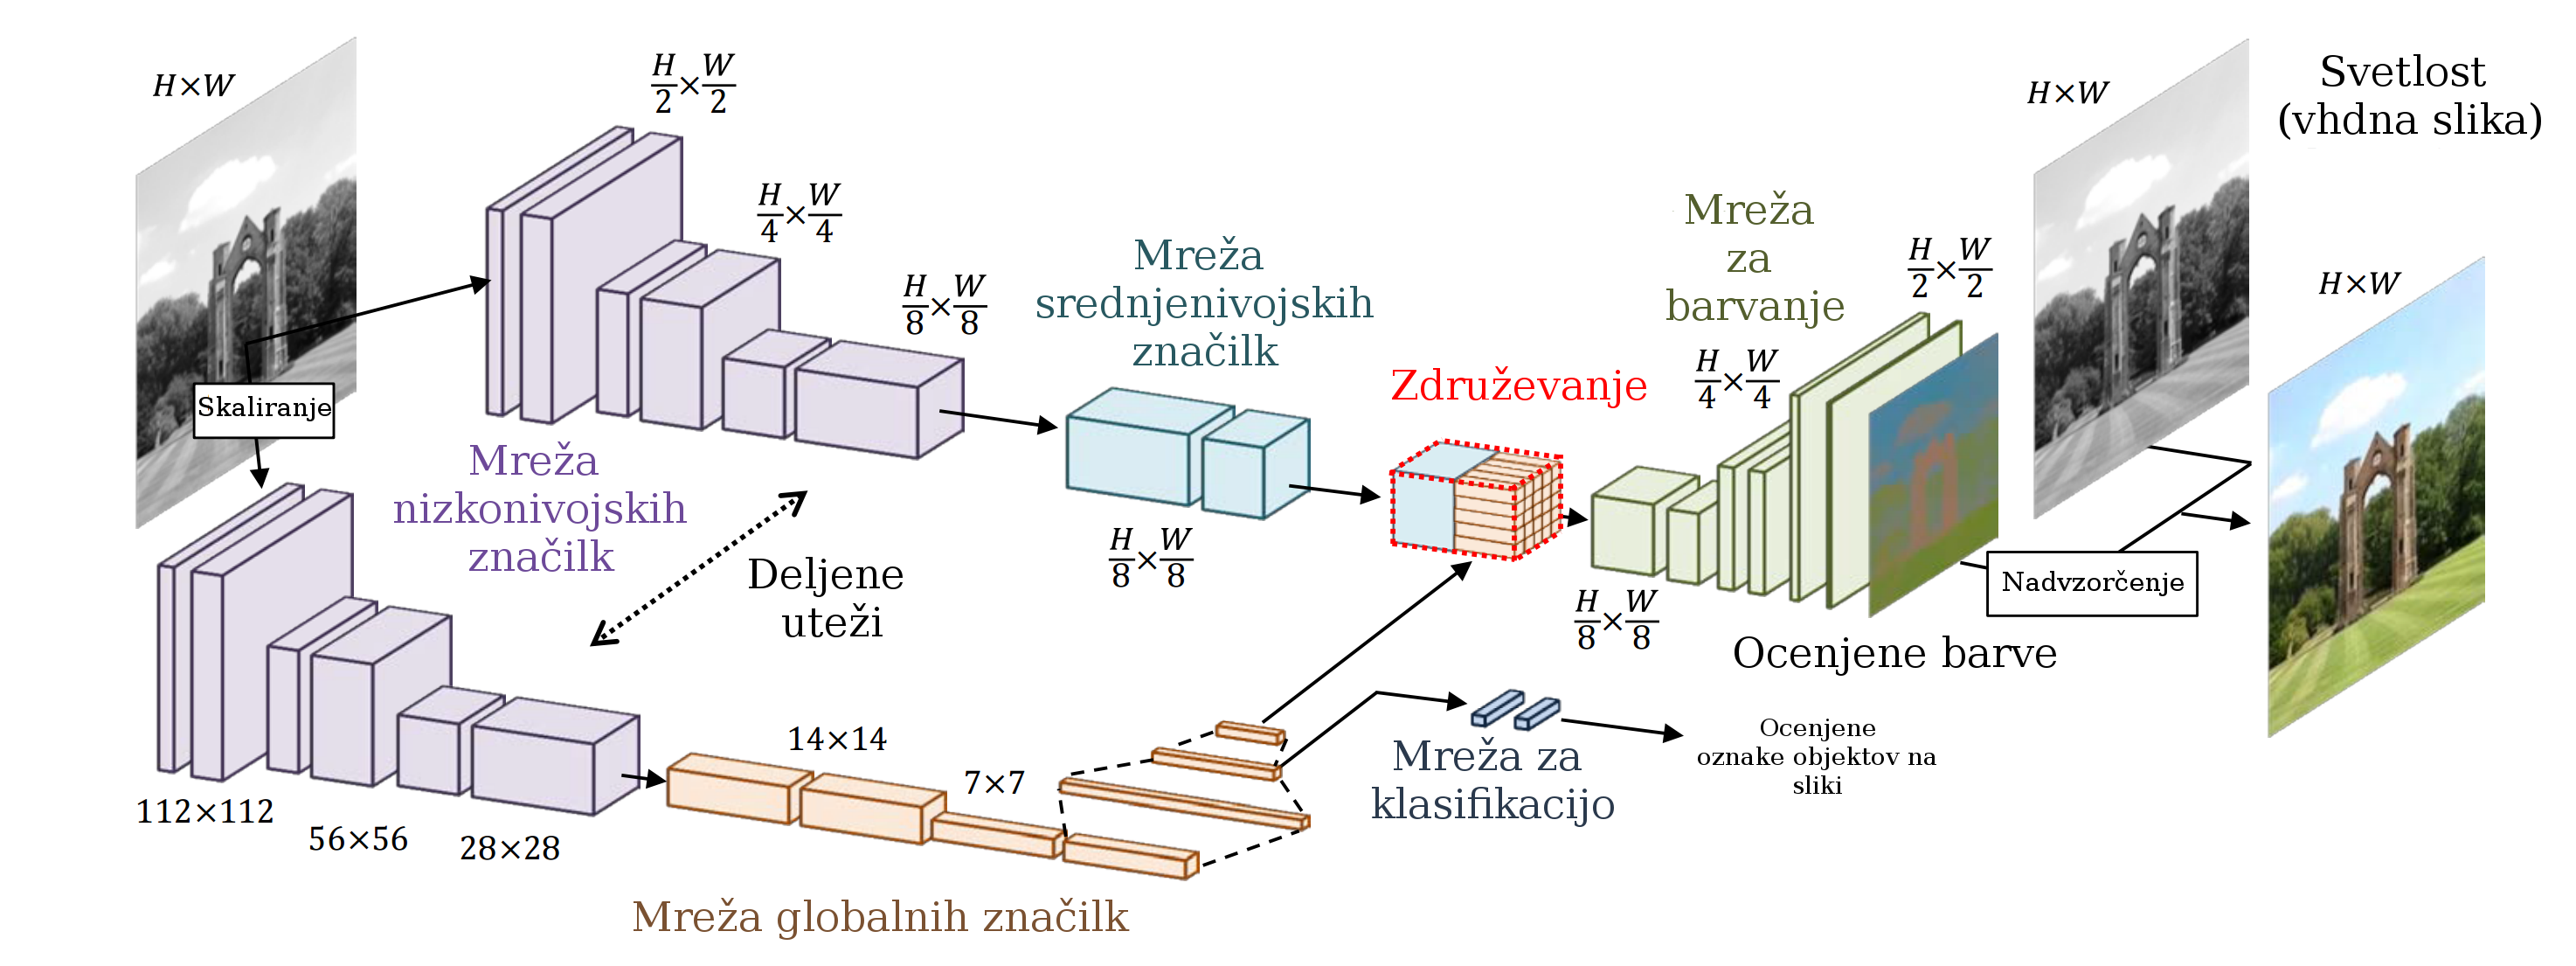
\includegraphics[width=13cm]{iizuka_arh}
\end{center}
\caption{Slika prikazuje arhitekturo mreže Iizuka in sod. \cite{Iizuka2016}. Mreža dobi na vhodu črno belo sliko. Ta se poda tako mreži za klasifikacijo spodaj, kot mreži za barvanje zgoraj. Obe mreži se združita v nivoju združevanja. Izhod mreže je slika z barvnimi komponentami $a*b*$, ki se nato združi s črno-belo sliko. Vir slike: Iizuka in sod. \cite{Iizuka2016}. }
\label{im:iizuka-arh}
\end{figure}


%----------------------------------------------------------------
% Poglavje (Chapter) 3: Pregled področja
%----------------------------------------------------------------

\chapter{Barvanje črno-belih slik z globokimi nevronskimi mrežami}
\label{ch:barvanje}

V nalogi smo preizkusili nekaj različnih arhitektur globokih nevronskih mrež. Razvili smo tako pristope z regresijo kot klasifikacijo. Razvili smo tudi pristop, ki zna učinkovito barvati slike večje od teh iz učne množice.

\section{Arhitekture nevronskih mrež}
\label{ch:arhitekture}

Implementirali smo štiri arhitekture nevronskih mrež in jih kombinirali z različnimi cenilnimi funkcijami, pristopi (regresijski ali klasifikacijski) in na\-či\-ni napovedovanja (napovedovanje po delih ali na celi sliki).

\subsection{Arhitektura S+G}
\label{ch:plitva}

Arhitektura S+G (Shallow with global) je sestavljena iz dveh delov, ki se kasneje združita v enotno mrežo. Glavni del predstavlja zaporedje konvolucijskih nivojev, ki na vhodu vzamejo črno-belo sliko z enim kanalom, izhod pa je obarvana slika z dvema kanaloma za barvni komponenti $a*$ in $b*$. Po prvih osmih kovolucijskih nivojih se mreža združi s tako imenovano globalno mrežo, ki prepoznava objekte na sliki. Za globalno mrežo smo vzeli že naučeno šestnajstnivojsko mrežo VGG-16 \cite{Simonyan2014}, ki smo ji odvzeli zadnji polnopovezani nivo in ji dodali nov polnopovezani nivo z izhodnim tenzorjem dolžine 256. Ker je arhitektura VGG-16 namenjena sprejemu barvnih slik s tremi vhodnimi kanali, smo vhod prilagodili tako, da sprejme sivinsko sliko na vsakem od vhodnih kanalov. Arhitektura nevronske mreže je predstavljena na sliki \ref{im:arh1} in z implementacijo v prilogi \ref{ch:app_sg}.

\begin{figure}[hbt]
\begin{center}
\centering
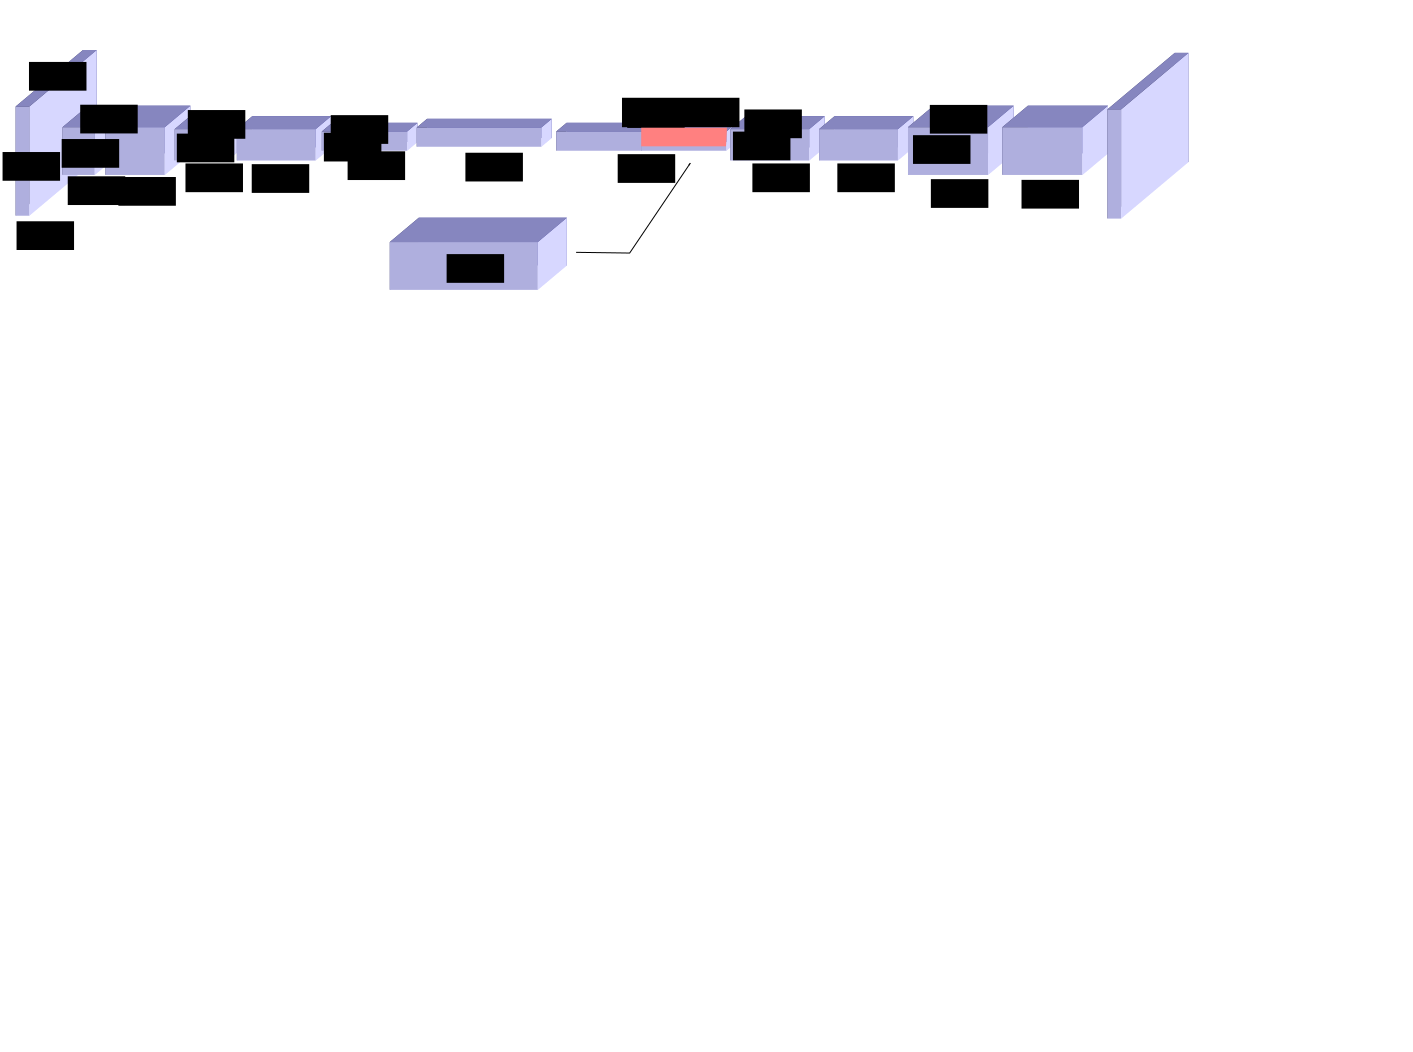
\includegraphics[width=13cm]{arh1}
\end{center}
\caption{Velikosti tenzorjev skozi arhitekturo S+G. Oznaki $h$ in $w$ predstavljata višino in širino vhodne slike. Podrobnosti nivoja združitev so predstavljene na sliki \ref{im:fusion}, nivo izhodne slike ni natančneje označen, saj se razlikuje v različnih implementacijah, ki so podrobneje opisane v poglavjih \ref{ch:regression-methods} in \ref{ch:classification-methods}. }
\label{im:arh1}
\end{figure}

Vhod v element za združevanje glavne in globalne mreže sta tenzorja velikosti $\frac{h}{8} \times \frac{w}{8} \times 256$ iz glavne mreže in enodimenzionalni tenzor velikosti $256$ iz globalne mreže. Pri tem $h$ in $w$ predstavljata višino in širino vhodne slike v mrežo. Pri združevanju vsakemu elementu širine in višine prvega tenzorja pridružimo tenzor globalne mreže (slika \ref{im:fusion}). Tako na izhodu dobimo tenzor velikosti $\frac{h}{8} \times \frac{w}{8} \times 512$. 
 
\begin{figure}[hbt]
\begin{center}
\centering
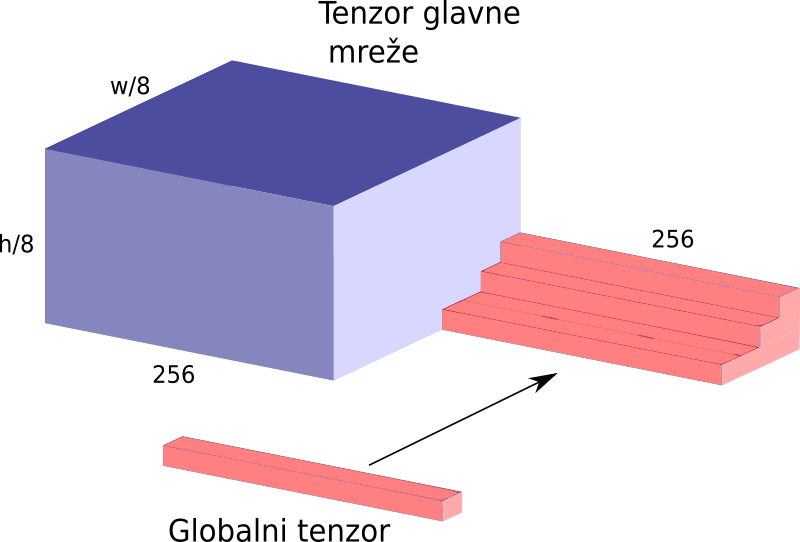
\includegraphics[width=8cm]{fusion-1}
\end{center}
\caption{Delovanje nivoja združevanja glavne nevronske mreže z globalno nevronsko mrežo. K izhodu glavne nevronske mreže (modri tenzor) dodamo tenzor iz globalne mreže (rdeči tenzor), tako da ga priključimo k vsem prostorskim lokacijam glavnega tenzorja kot dodatnih 256 kanalov. Izhodni tenzor ima tako velikost $\frac{h}{8} \times \frac{w}{8} \times 512$.}
\label{im:fusion}
\end{figure}

% l2 regularizacija citation \cite{mackay1992practical}

\subsection{D+G arhitektura}
\label{ch:globjaz}

D+G (Deep with global) arhitektura ima v osnovi enako zasnovo, kot arhitektura v poglavju \ref{ch:plitva}. Razlika se pojavi pri globini glavne mreže. Ta ima namreč 14 konvolucijskih nivojev pred združitvijo in 7 po združitvi (slika \ref{im:arh2} in priloga \ref{ch:app_dg}). 

Za razliko od arhitekture opisane v poglavju \ref{ch:plitva} ta za zmanjševanje prostorskih (ang. {\em spatial}) dimenzij uporablja maksimalno združevanje (ang. {\em max pooling}) \cite{Krizhevsky2012} in za povečevanje le teh v zadnjih nivojih uporablja transponirano konvolucijo (ang. {\em transpose convolution}) \cite{Dumoulin2016} imenovano tudi dekonvolucija. Transponirana konvolucija je transformacija, ki deluje v nasprotni smeri kot običajna konvolucija. Torej na vhodu vzame tenzor dimenzije, ki je izhod konovlucije z enakimi parametri, izhod transponirane konvolucije pa je tenzor dimenzije enake tistemu na vhodu običajne konvolucije. Transponirana konvolucija za svoje delovanje še vedno uporablja princip konvolucije. Združevanja glavne in globalne mreže se izvede kot je opisano v poglavju \ref{ch:plitva}.

Arhitektura D+G prinaša še eno spremembo. To so tako imenovane rezidualne povezave, ki so bile prvič uporabljene v nevronski mreži ResNet, zasnovani s strani Microsoft Research Asia \cite{Wu2017}, ki je leta 2015 zmagala na tekmovanju ImageNet \cite{ILSVRC15}. Te povezave so na sliki \ref{im:arh2} označene s puščicami nad nevronsko mrežo in predstavljajo povezavo, ki na mestu, kamor kaže puščica, združi trenutni tenzor s tenzorjem izračunanim pred dvema nivojema. Operacija združevanja pomeni seštevanje isto ležečih elementov v tenzorju. Za rezidualne povezave smo se odločili, saj naj bi te prisilile nivoje, da se naučijo nekaj novega in ne le nadgradijo izhod prejšnjega nivoja, s tem smo računali na izboljšavo v natančnosti barvanja.

\begin{figure}[hbt]
\begin{center}
\centering
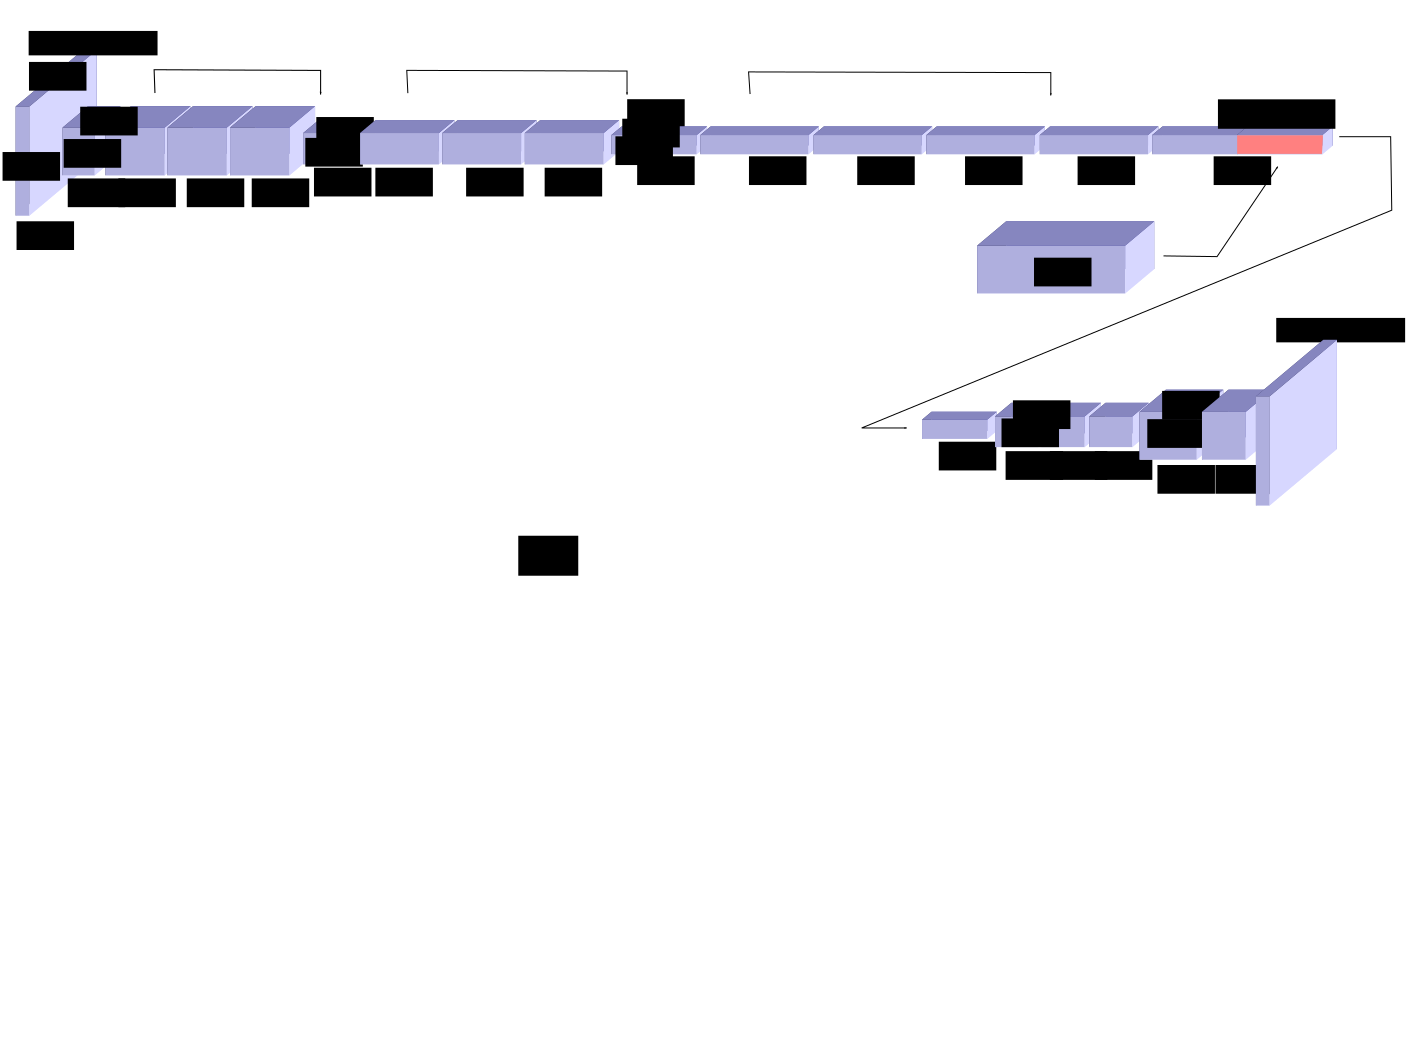
\includegraphics[width=13cm]{arh2}
\end{center}
\caption{Velikosti tenzorjev skozi arhitekturo D+G. Oznaki $h$ in $w$ predstavljata višino in širino vhodne slike. Podrobnosti nivoja združitev so predstavljene na sliki \ref{im:fusion}, nivo izhodne slike ni natančneje označen, saj se razlikuje v različnih implementacijah, ki so podrobneje opisane v v poglavjih \ref{ch:regression-methods} in \ref{ch:classification-methods}. }
\label{im:arh2}
\end{figure}

\subsection{Arhitektura D}

Ta arhitektura je v glavnem delu enaka tisti opisani v poglavju \ref{ch:globjaz} in prikazani na sliki \ref{im:arh2}. Razlikuje se po tem, da nima globalne mreže. To pomeni, da nima mreže, ki bi se pridružila v nivoju združitve, zaradi tega smo ta nivo izpustili. Mreža za vhod vzame črno-belo sliko z enim kanalom in izračuna barvno sliko na izhodu samo preko konvolucijskih nivojev. Ta arhitektura je bila načrtovana z namenom preverjanja vpliva globalne mreže na rezultate barvanja.

\subsection{Arhitektura X-VGG}

Arhitektura X-VGG je zgrajena tako, da za nižje nivoje uporabimo mrežo VGG-16 \cite{Simonyan2014}, kateri smo odstranili vse polnopovezane nivoje. Arhitektura je narejena tako, da na vhodu sprejme črno-belo sliko, ki jo potem prilagodimo za vhod mreže VGG-16, tako da ima tri vhodne kanale. Te pridobimo tako, da vzamemo sivinsko sliko za vsak vhodni kanal. Tenzor, ki ga vrne zadnji konvolucijski nivo mreže VGG-16, podamo na vhod prvega nivoja lastne mreže, ki je prikazana na sliki \ref{im:arh4} in v prilogi \ref{ch:app_xvgg}. Lastna mreža ima še osem konvolucijskih nivojev in štiri nivoje nadvzorčenja, ki poskrbijo za povečanje dimenzije prostorskih komponent. Po zadnjem nivoju izvedemo še povečanje slike za faktor dve, saj se nadvzorčenje izkaže kot slabša možnost.

\begin{figure}
\begin{center}
\centering
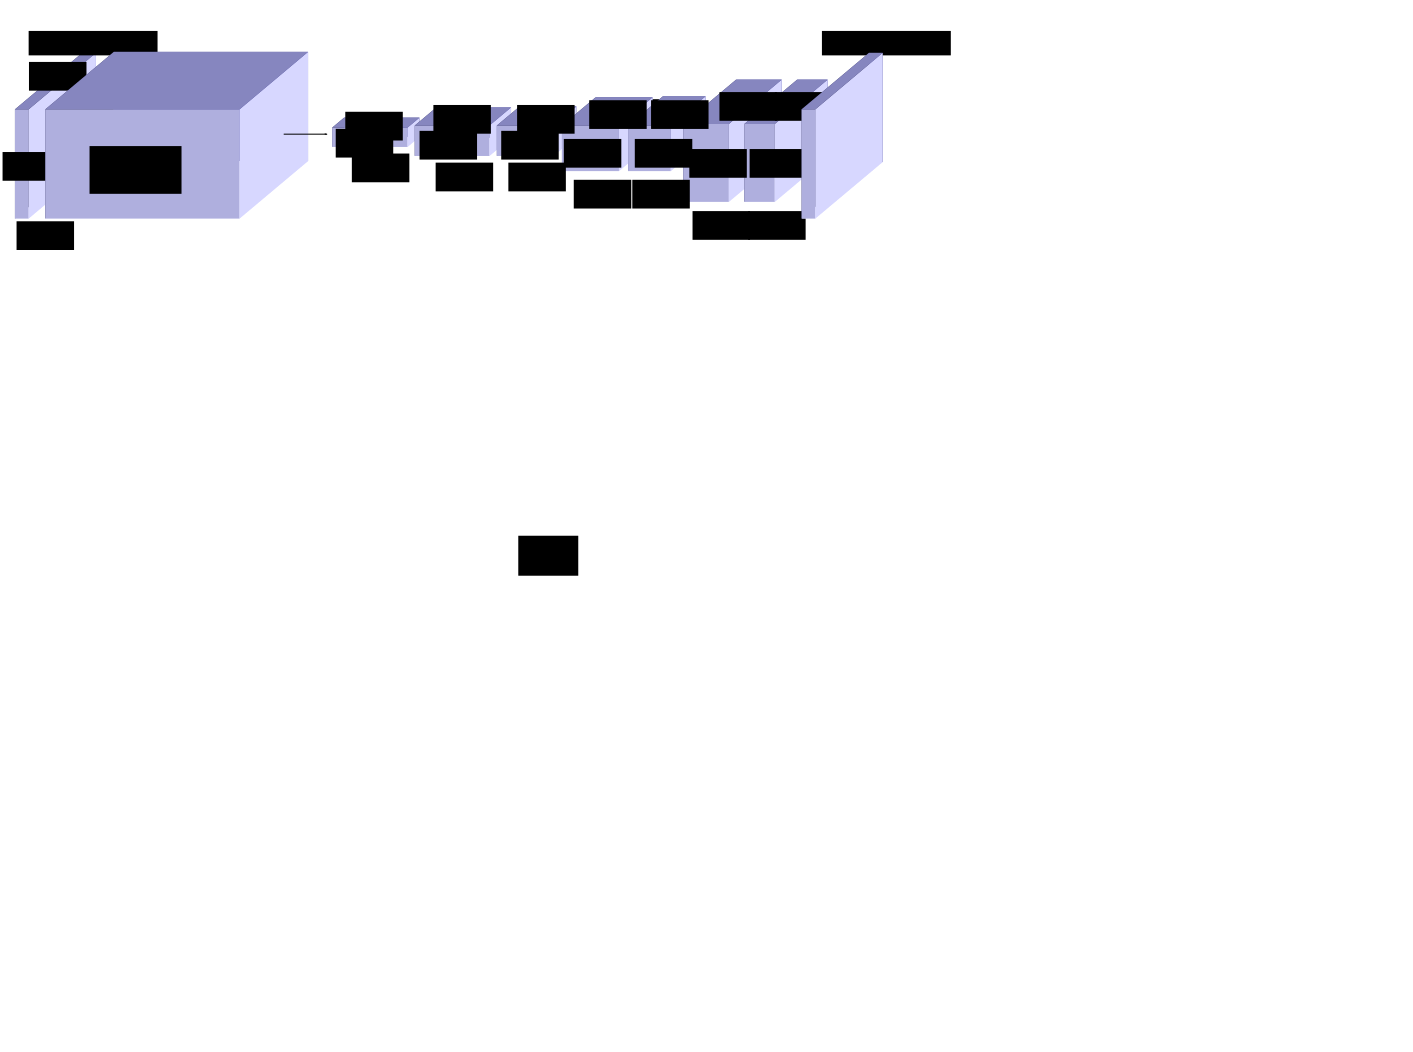
\includegraphics[width=12cm]{arh4}
\end{center}
\caption{Velikosti tenzorjev skozi arhitekturo X-VGG. Oznaki $h$ in $w$ predstavljata višino in širino vhodne slike. Nivo izhodne slike ni natančneje označen, saj se razlikuje v različnih implementacijah, ki so podrobneje opisane v poglavjih \ref{ch:regression-methods} in \ref{ch:classification-methods}. Prvi večji blok predstavlja mrežo VGG-16 \cite{Simonyan2014}}
\label{im:arh4}
\end{figure}

\section{Pristopi z regresijo}
\label{ch:regression-methods}

V tem poglavju bomo prestavili uporabljene regresijske pristope. Ti pri napovedovanju direktno napovejo vrednosti $a*$ in $b*$ barvne komponente v prostoru CIE L*a*b*. Tu mreža predstavlja regresijsko funkcijo $Y = f(X)$ za vsako točko slike, ki na vhod dobi točko sivinske slike $X$, izhod pa sta vrednosti $a*$ in $b*$.

Na sliki \ref{im:reg-scheme} je prikazan postopek delovanja, ki je skupen vsem regresijskim pristopom opisanim v nadaljevanju. Da dobimo barvno sliko, mreži podamo sivinsko sliko, ta oceni barvni komponenti $a*$ in $b*$, nato izhod mreže združimo z sivinsko sliko, ki je obenem komponenta $L*$. Rezultat je obarvana slika. 

\begin{figure}[hbt]
\begin{center}
\centering
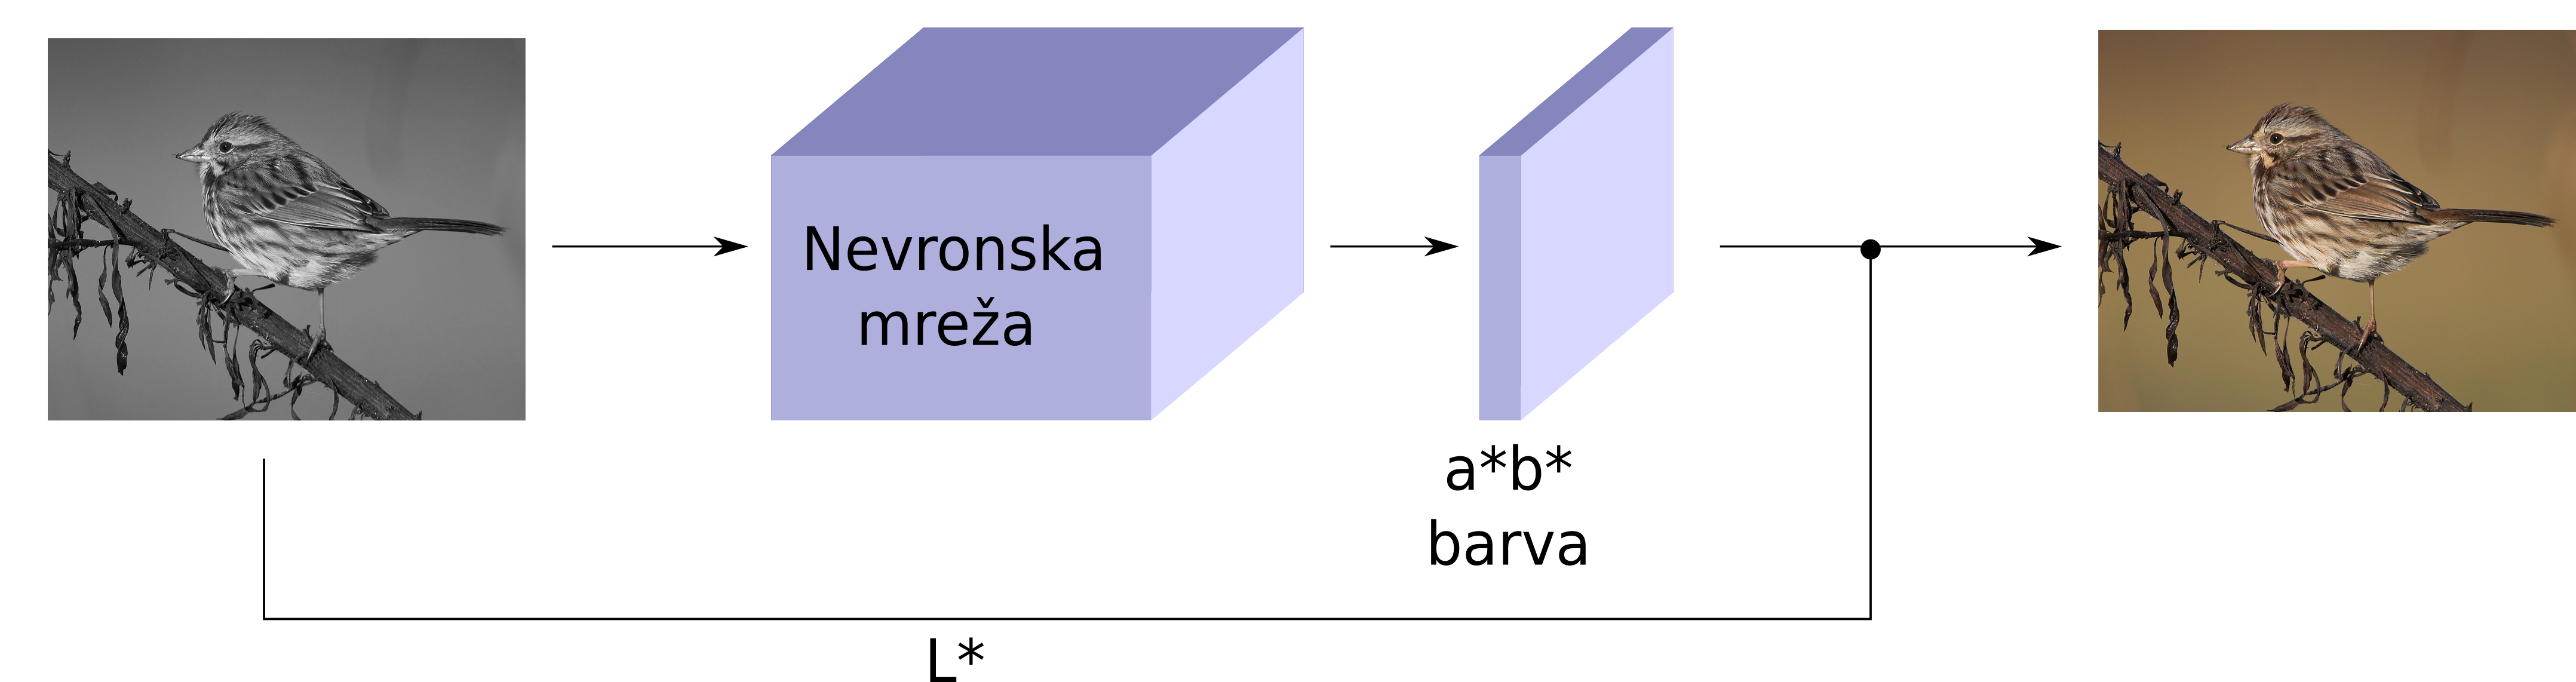
\includegraphics[width=13cm]{regresija-shema}
\end{center}
\caption{Regresijski pristopi na vhod prejmejo črno-belo sliko in s pomočjo nevronske mreže izračunajo barvni komponenti $a*$ in $b*$ barvnega prostora \textit{CIE L*a*b*}. }
\label{im:reg-scheme}
\end{figure}

\subsection{Pristopi na delih slik}
\label{ch:parts-im}

Barvanje pri tem pristopu izvedemo ločeno na majhnih delih slik. Motivacija za to je imitacija, kako se barvanja loti človek, na sliki bi namreč zaznal objekte in jih ločeno obarval. Najprej bi na primer obarval vodo, nato gozd in kasneje še nebo. 

Preden sliko podalmo nevronski mreži, jo razdelilmo na koščke velikosti $32 \times 32$ slikovnih točk. Pri tem se sosednja koščka prekrivata za $16$ slikovnih točk, kot je prikazano na sliki \ref{im:overlapping}. 
V arhitekturah, kjer je prisotna ločena globalna mreža, ta še vedno na vhodu prejme celotno sliko, s katero pridobimo globalni koncept slike. Dele slik po barvanju sestavimo z metodo prekrivanja, tako da imajo vrednosti točk pri robu manjši vpliv kot tiste pri sredini. Vpliv barvne točke se izračuna po enačbi \ref{eq:1}, kjer $Y_{h, w}$ predstavlja vrednost slikovne točke, $d$ pa predstavlja oddaljenost od središča v številu slikovnih točk. Enačba se ločeno uporablja v vertikalni in horizontalni smeri. Da dobimo končno vrednost v določeni točki, seštejemo vse prispevke za tisto točko utežene po enačbi \ref{eq:1}.

\begin{equation}
Y'_{h, w} = \frac{d}{16} Y_{h, w}
\label{eq:1}
\end{equation}

\begin{figure}[hbt]
\begin{center}
\centering
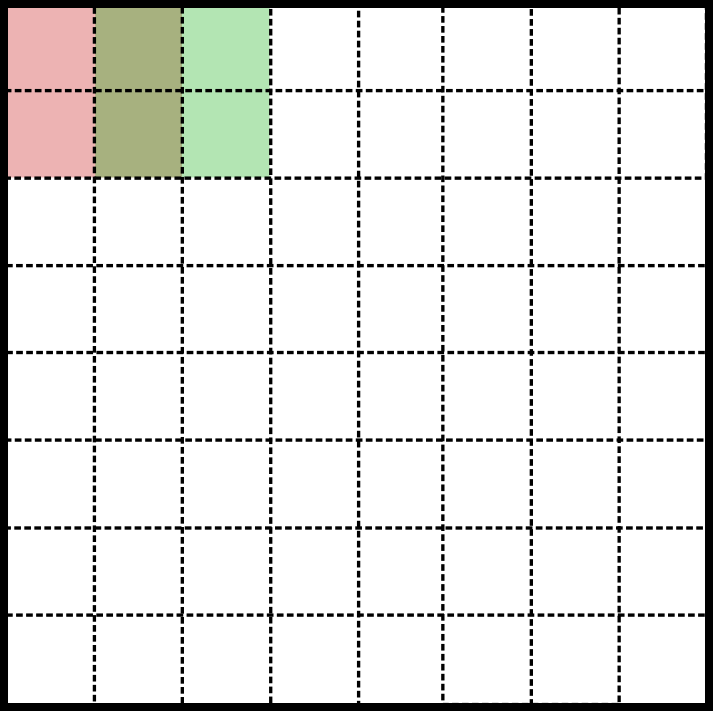
\includegraphics[width=6cm]{overlapping1}
\end{center}
\caption{Razdelitev slike velikosti $128 \times 128$ slikovnih točk, na $7 \times 7$ enakih delov velikosti $32$ slikovnih točk, ki se med seboj v vseh smereh prekrivajo za $16$ slikovnih točk. Rdeč in zelen kvadrat prikazujeta prvi dve podsliki.}
\label{im:overlapping}
\end{figure}

S predlaganim pristopom pričakujemo pohitritev učenja, saj menimo, da je že del slike dovolj, da se mreža nauči celotne teksture objekta. Na primer, da se naučimo barvati vodo ne potrebujemo celotnega območja vode na sliki, ki včasih lahko zavzema tudi pol ali več slike, ampak le en del. Z učenjem mreže na manjših vhodnih tenzorjih, kar dosežemo z učenjem po delih, se čas, ki ga mreža porabi za učenje ene serije (ang. {\em batcha}) podatkov, zmanjša.

V tabeli \ref{tab:learning-speed} so prikazani časi potrebni za učenje pri dveh regresijskih pristopih, ki se razlikujeta le v tem, da en uči po delih, drugi pa na celih slikah. Oba pristopa sta bila učena ob istem času na isti napravi in ločenih GPU enotah. Iz tabele je razvidno, da pristop po delih potrebuje krajši čas, da se nauči barvanja. Ta čas je krajši skoraj za faktor tri. To pripišemo predvsem  krajšemu času potrebnemu za en korak učenja, število korakov do naučenega pristopa pa je podobno.

\begin{table}[hbt]
\caption{Povprečen čas enega koraka (prehod preko 50.000 slik) pri učenju pristopov, število prehodov potrebnih za učenje in skupni čas potreben za učenje. Rezultati so prikazani za dva regresijska pristopa z enakimi arhitekturami, oba imata arhitekturo D+G in drugačnim načinom učenja. Iz rezultatov je razvidno, da pristopi po delih za konvergenco potrebujejo manj časa.}
\begin{center}
    \begin{tabular}{lccc}
    \hline
	Pristop & Čas za korak [s] & Št. korakov & Skupni čas za učenje [s]\\
	\hline
	Po delih & 619,8 & 90  & 55.782\\
	Cela slika  & 1815,0 & 89 & 161.535\\
	\hline
    \end{tabular}
\end{center}
\label{tab:learning-speed}
\end{table}

V tabeli \ref{tab:methods-whole} so predstavljene podrobnosti vsakega od pristopov barvanja po delih. Vsem pristopom je skupno, da uporabljajo cenilno funkcijo povprečna kvadratna napaka (MSE).


\subsection{Pristopi na celih slikah}

Za primerjavo točnosti pristopov na delih slik s tistimi na celih slikah, smo dva pristopa opisana v poglavju \ref{ch:parts-im} pretvorili v pristop za barvanje na celih slikah. Uporabili smo  arhitekturi D+G in D, ki smo jih prilagodili tako, da na vhodu sprejmeta celotno sivinsko sliko in vrne celotno obarvano sliko. Tej smo dodali še regresijski pristop na celi sliki z mrežo VGG, saj ta zaradi večkratnega pomanjšanja prostorskih dimenzij znotraj arhitekture, ne more biti realiziran na manjših delih slik. V tabeli \ref{tab:methods-whole} so podrobno predstavljene arhitekture in cenilne funkcije teh pristopov. 

\begin{table}[hbt]
\caption{Regresijski pristopi in njihove arhitekture, ki so podrobneje opisane v poglavju \ref{ch:arhitekture}.}
\begin{center}
\begin{tabular}{lcc}
\hline
Pristop & Arhitektura & Cenilna funkcija \\
\hline
	Reg. po delih & D+G & MSE \\
	\hspace{0.5em} - brez softmax & D+G & MSE \\
	\hspace{0.5em} - brez globalne mreže & D & MSE \\
\hline
Reg. cela slika & D+G. & MSE \\
\hspace{0.5em} - brez globalne mreže & D & MSE \\
Reg. cela slika VGG & X-VGG & MSE \\
\hline
\end{tabular}
\end{center}
\label{tab:methods-whole}
\end{table}

\section{Pristopi s klasifikacijo}
\label{ch:classification-methods}

Razvili smo štiri pristope, ki namesto regresije uporabljajo klasifikacijo. Pri teh pristopih barvo ocenimo z izbiro najbolj primernega razreda, ki predstavlja nekaj sosednjih odtenkov. Posamezen razred opiše barve, ki so blizu skupaj v dvodimenzionalnem prostoru a*b*.
Klasifikacija se izvede z uporabo \textit{softmax} funkcije v zadnjem nivoju mreže. 

Kot je prikazano na sliki \ref{im:class-scheme}, je vhod v metodo črno-bela slika, ki se posreduje nevronski mreži. Ta oceni obarvanje kot vektor verjetnosti za vsakega od razredov vsake slikovne točke. Te vrednosti se potem pretvorijo v $a*$ in $b*$ komponenti barvnega prostora CIE L*a*b*. Enako kot pri regresiji je rezultat združitev sivinske slike z ocenjenimi barvnimi komponentami. 

\begin{figure}[hbt]
\begin{center}
\centering
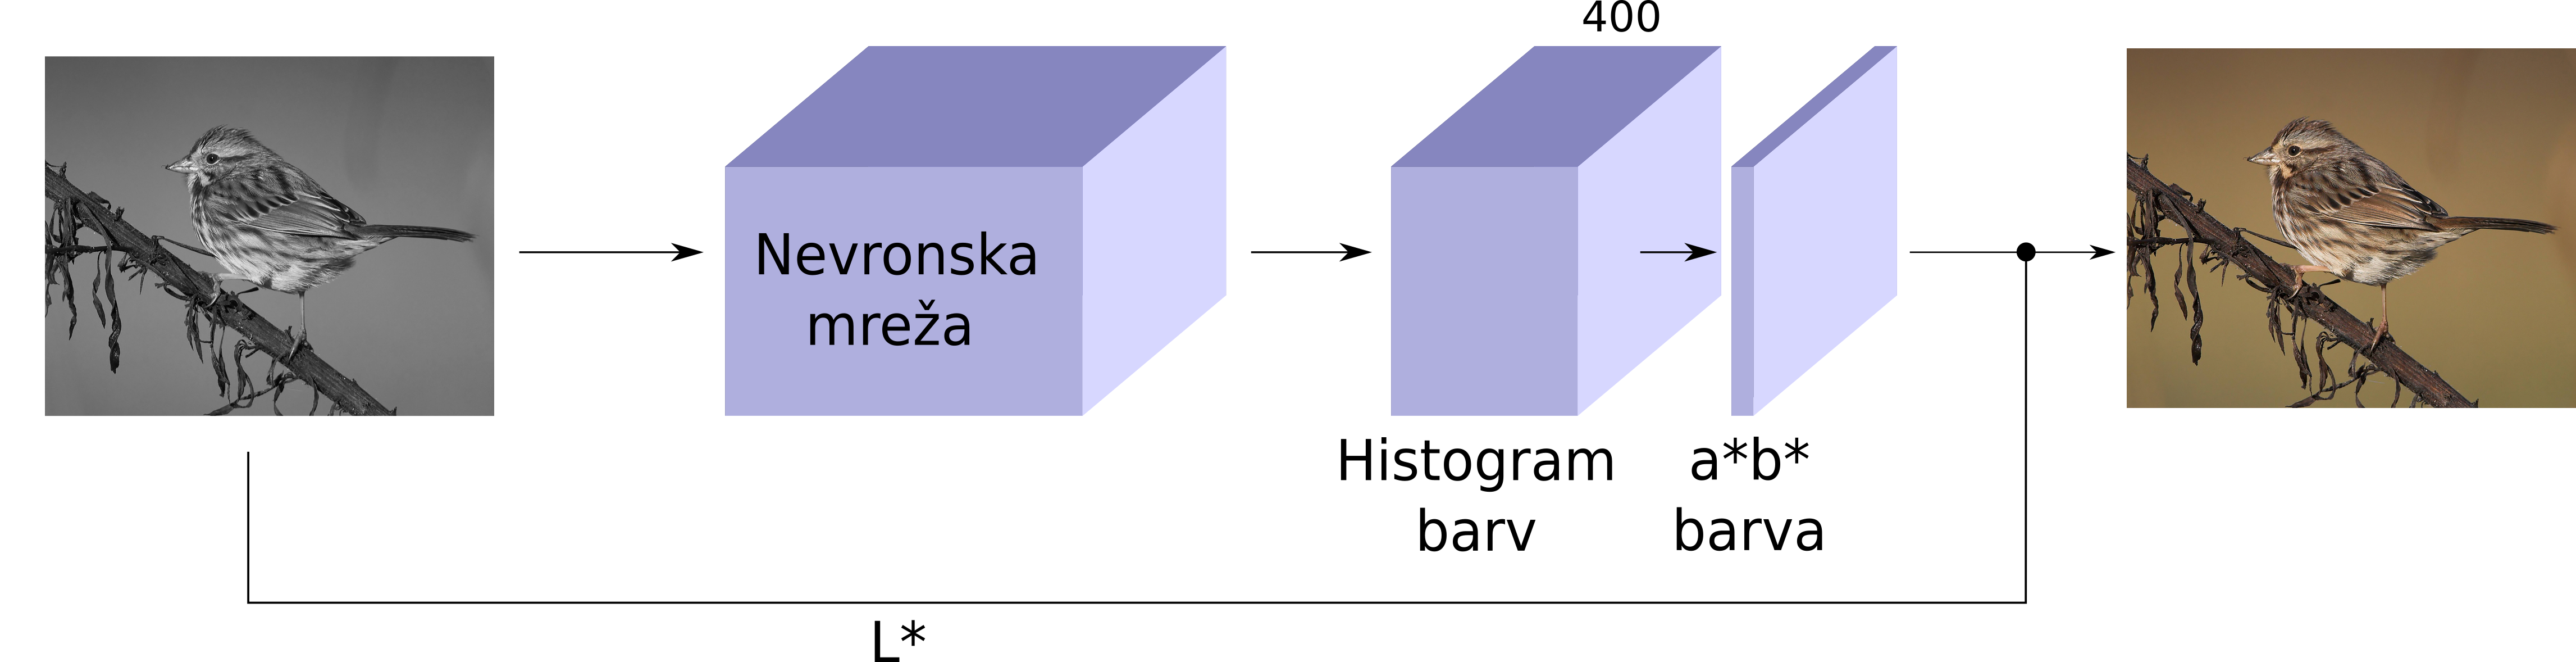
\includegraphics[width=13cm]{classification-scheme}
\end{center}
\caption{Shematski prikaz delovanja klasifikacijskih  pristopov, ki na vhodu prejmejo črno-belo sliko, s pomočjo nevronske mreže izračunajo verjetnosti za posamezen razred barv (histogram), te potem pretvorijo v barvni komponenti $a*$ in $b*$ barvnega prostora CIE L*a*b*, te pa nato združijo s sivinsko sliko $L*$, da dobijo obarvano sliko.}
\label{im:class-scheme}
\end{figure}

Razrede smo dobili tako, da  komponenti $a*$ in $b*$ barvnega prostora CIE L*a*b* razdelimo v $400$ razredov, kar se je izkazalo za najbolje, saj s $400$ razredi lahko barve zapišemo tako, da izgub zaradi nenatančnega kodiranja uporabnik ne bo opazil, večje število razredov, pa bi preveč upočasnilo učenje in napovedovanje. Vsako od komponent smo razdelili v $20$ razredov med vrednostima $-100$ do $100$, kar pomeni, da vsak razred zajema interval širine $10$. Vse kombinacije obeh komponent prinesejo $400$ razredov.

Pretvorba iz zapisa $a*b*$ v histogram se uporabi pri učenju, kjer originalno sliko pretovorimo v histogram, da lahko izračunamo napako. To izvedemo z enačbo \ref{eq:ab2hist}, kjer $a$ in $b$ predstavljata $a*$ in $b*$ vrednost slikovne točke, $l$ pa indeks razreda v histogramu, ki zavzema cela števila v intervalu $[0, 399]$. 

\begin{equation}
l = 20 \left\lfloor\frac{a + 100}{10} \right\rfloor + \left\lfloor\frac{b + 100}{10} \right\rfloor
\label{eq:ab2hist}
\end{equation}

Pretvorba iz histograma v $a*$ in $b*$ se uporabi pri pretvorbi ocenjenih barvnih vrednosti s strani mreže in se izvede skladno z enačbo \ref{eq:hist2ab}. Pri tem $a$ in $b$ predstavljata $a*$ in $b*$ barvne vrednosti slikovne točke, $l$ pa predstavlja indeks razreda v histogramu, ki je bil napovedan z največjo verjetnostjo. Vsem komponentam dodamo še vrednost $5$, tako da dobimo barvne vrednosti iz sredine vsakega razreda.

\begin{equation}
\begin{gathered}
a = 10 \left\lfloor \frac{l}{20} \right\rfloor - 100 + 5 \\
b = 10 (l \mod 20)  - 100 + 5
\end{gathered}
\label{eq:hist2ab}
\end{equation}

V tabeli \ref{tab:methods-class} so prikazani pristopi s klasifikacijo, njihova arhitektura in cenilna funkcija. Vsi pristopi s klasifikacijo uporabljajo princip barvanja po delih.

\begin{table}[hbt]
\caption{Klasifikacijski pristopi po delih, njihove arhitekture, ki so podrobneje opisane v poglavju \ref{ch:arhitekture} in cenilne funkcije uporabljene za učenje. Podrobnosti cenilnih funkcij je možno najti v poglavju \ref{ch:cenilne}}
\begin{center}
    \begin{tabular}{lcc}
  	\hline
	Pristop & Arhitektura & Cenilna funkcija \\
	\hline
	Klas. brez uteži - S+G. & S+G &  KL-divergenca \\
	Klas. brez uteži - D+G & D+G & CE \\
	Klas. z utežmi - S+G & S+G & CEw \\
	Klas. z utežmi - D+G & D+G mr. & CEw \\
	\hline
    \end{tabular}
\end{center}
\label{tab:methods-class}
\end{table}

%----------------------------------------------------------------
% Poglavje (Chapter) 4: Vrednotenje
%----------------------------------------------------------------

\chapter{Vrednotenje}

\section{Postopek učenja}

V tem poglavju bomo predstavili podrobnosti učenja na manjši množici, na večji učni množici in si za konec pogledali kakšne značilke prepozna posamezen nivo nevronske mreže. 

Za posodabljanje uteži mreže smo uporabili optimizator Adam, ki je trenutno najbolj v uporabi na nivoju nevronskih mrež. Pri tem so se za dobre izkazali parametri, ki so prikazani v tabeli \ref{tab:adam-param}. Pri vseh pristopih smo uporabili velikost serije (ang. {\em batch size}) $32$, razen pri učenju metode Zhang in sod., kjer smo morali zaradi večjih dimenzij tenzorjev in posledično pomakanju pomnilnika uporabiti velikost serije $8$.

\begin{table}[hbt]
\caption{Parametri, s katerim smo nastavili Adam optimizatior. }
\begin{center}
\begin{tabular}{lcc}
\hline
Parameter & Vrednost parametra \\
\hline
stopnja učenja (ang. {\em learning rate}) & $10^{-4}$ \\ 
beta 1 & $0,9$ \\
beta 2 & $0,99$ \\ 
epsilon & $10^{-8}$ \\
\hline
\end{tabular}
\end{center}
\label{tab:adam-param}
\end{table}

Za učenje na manjši učni množici smo izbrali vse pristope, za učenje na večji učni množici smo izbrali sedem pristopov, pet lastnih in dva iz sorodnih del. Manjša in večja učna množica sta podrobno opisani v poglavju \ref{ch:podatki}. Odločili smo se za tri regresijske pristope: regresija po delih z globalno mrežo, regresija na celotni sliki z globalno mrežo in regresija na celotni sliki z mrežo VGG-16. Izpustili smo oba pristopa brez globalne mreže, saj imata očitno slabše rezultate barvanja. 
Izbrali smo dva klasifikacijska pristopa klasifikacija brez uteži - S+G in klasifikacija z utežmi - S+G, namreč izkazalo se je, da  arhitektura D+G poslabša rezultate, zato smo se odločili, da izvedemo le primerjavo dveh pristopov z arhitekturo S+G. 

%----------------------------------------------------------------
% Section: Podatki
%----------------------------------------------------------------

\section{Barvanje večjih slik}
\label{ch:vecjih}

Večina pristopov v sorodnih delih je naučenih za barvanje slik velikosti $224 \times 224$ in ima to omejitev, da omogoča le barvanje slik te velikosti. Iizuak in sod. \cite{Iizuka2016} omogočajo barvanje večjih slik, tako da večjo sliko podajo enaki mreži na vhod, ki nima omejitve za velikosti vhodne slike, saj je sestavljena le iz konvolucijskih nivojev. Pri tem avtorji komentirajo, da mreža deluje najbolje na slikah velikosti $224 \times 224$.

S pristopi po delih, ki smo jih implementirali v okviru tega dela, ta problem rešujemo drugače. Slike katerekoli velikosti večjih od $32 \times 32$ razdelimo na dele velikosti $32 \times 32$ s prekrivanjem, jo obarvamo po delih in potem spet sestavimo po principu opisanem v poglavju \ref{ch:parts-im}.

Primerjavo kakovosti barvanja večjih slik smo izvedli tako, da smo pristopa Iizuka in sod. ter regresijo po delih z globalno mrežo preizkusili na istih slikah pomanjšanih na velikost $224 \times 224$ slikovnih točk, kjer naj bi bilo barvanje optimalno in velikost $896 \times 896$. Primerjava je izvedena na mrežah naučenih na manjši učni množici s $100 000$ slikami. 

\section{Podatki}
\label{ch:podatki}

Podatke, ki smo jih uporabili za učenje in validacijo pristopov smo pridobili iz podatkovne zbirke ImageNet \cite{ILSVRC15}, ki vsebuje približno $14$ milijonov slik. Iz zbirke smo naključno izbrali množico podatkov in jih za namen učenja pretvorili v barvni prostor CIE L*a*b*. Pri preizkusu na manjši množici smo za učenje naključno izbrali $100.000$ slik in za validacijo pa $10 000$ slik iz nabora. Validacijska množica je bila obenem tudi testna množica. Za učenje na večji množici smo naključno izbrali $2.854.912$ slik, za validacijo smo še vedno uporabljali $10.000$ slik, ki so bile obenem tudi testna množica.

Za namen testiranja barvanja večjih slik, opisanega v poglavju \ref{ch:vecjih}, podatki iz podatkovne zbirke Imagenet niso bili zadovoljivi, saj so slike večinoma velikosti manjših od $500 \times 500$ slikovnih točk. Odločili smo se, da testiranje izvedemo na lastnih slikah, ki so večje od velikosti $896 \times 896$, kar pomeni, da slik ni potrebno povečevati in s tem povzročati dodatnih napak v barvanju zaradi slabe kvalitete slik. Za namen testiranja smo vzeli $584$ slik, katere je aplikacija Google Photos\footnotemark{} ocenila, da gre za slike pohodništva. Za te slike smo se odločili, ker gre večinoma za slike narave, kjer je barvanje ponavadi najboljše in lahko razliko opazujemo na slikah, ki se večinoma barvajo dobro. 

\footnotetext{\url{http://photos.google.com}}

Za preizkus na starih črno-belih slikah smo izbrali raznovrstne slike iz dveh člankov iz spleta in zbirke starih črno-belih slik:
40 Must-See Photos From The Past\footnote{\url{http://www.boredpanda.com/must-see-historic-moments/}}, 
37 Wonderfully Weird Old Photos That Show Just How Much We’ve Changed\footnote{\url{http://www.lifebuzz.com/old-photos/}} in Old Photo Archive\footnote{\url{http://oldphotoarchive.com/}}.


%----------------------------------------------------------------
% Section: Racunanje napake
%----------------------------------------------------------------

\section{Računanje napake}
\label{ch:napake}

Za primerjavo pristopov smo napake računali na testni množici. Pri tem smo uporabili dve metrike: koren povprečne kvadratne napake (ang. {\em root mean squeared error}) in razmerje med signalom in šumom (ang. {\em peak signal-to-noise ratio}).  

Koren povprečne kvadratne napake (RMSE) za vsako sliko smo izračunali s pomočjo enačbe \ref{eq:rmse}, kjer $h$ in $w$ prestavljata višino in širino slike ter $c$ predstavlja število kanalov slike. Oznaka $Y$ predstavlja originalno sliko (ang. {\em ground truth}) in $\hat{Y}$ obarvano sliko s strani pristopa za barvanje. Napaka je bila izračunana za vsako sliko posebej in kasneje povprečena preko vseh slik. Napaka RMSE je bila izračunana na slikah v barvnem prostoru CIE L*a*b* le za $a*$ in $b*$ barvni kanal, saj za $L*$ barvni kanal izračun napake ni smiseln, ker so to vrednosti iz sivinske slike. 

\begin{equation}
\textrm{RMSE} = \sqrt{\sum^{h}_{i=1} \sum^{w}_{j=1} \sum^{c}_{k=1} (Y_{i, j, k} - \hat{Y}_{i, j, k})}
\label{eq:rmse}
\end{equation} 

Razmerje med signalom in šumom (PSNR) je metrika, ki kaže razmerje med največjo možno močjo signala in močjo šuma, ki signal pokvari. Primerna je za primerjave rekonstruiranih podatkov, kot so v našem primeru validacijske slike, ki jih poskušamo rekonstruirati s pomočjo pristopov, ki bazirajo na nevronskih mrežah. Vrednosti razmerja med signalom in šumom se merijo v enoti decibel ($dB$) \cite{Saupe2006}. Zadovoljive vrednosti rekonstrukcije slike $8$ bitnih podatkov, med kar sodijo tudi naši podtki, saj smo primerjali slike v barvnem prostoru \textit{RGB}, so med $30$ in $50$ dB \cite{welstead1999fractal}. 

Napako PSNR smo izračunali z enačbo \ref{eq:psnr}, v kateri ima $MAX_I$ največjo možno vrednost slikovne točke, kar je v barvnem prostoru RGB $255$, $\textrm{RMSE}$ pa je napaka izračuana z enačbo \ref{eq:rmse}. Napako smo povprečili preko vseh slik v testni množici. Za izračun napake smo izbrali barvni prostor RGB, saj računanje PSNR v prostoru L*a*b* ni možno, ker ne poznamo največje možne vrednosti signala za komponenti $a*$ in $b*$.

\begin{equation}
\textrm{PSNR} = 20 \log_{10}\left(\frac{MAX_I}{\textrm{RMSE}}\right)
\label{eq:psnr}
\end{equation}


\section[Primerjava pristopov glede na realističnost barvanja]{Primerjava pristopov glede na \\ realističnost barvanja}

Izkaže se, da številčna napaka, izračunana s primerjavo z originalno sliko, ni vedno dobra metrika za kvaliteto barvanja, saj bolj kot natančno obarvane slike, želimo slike, ki izgledajo realistično in naravno. Številčna napaka ni najboljša metrika predvsem v naslednjih primerih:

\begin{itemize}

\item Nekateri objekti na sliki imajo lahko različne barve, zato v primeru, ko algoritem pobarva z drugačno, a še vedno smiselno barvo, primerjava z originalno sliko ne da pravilne ocene napake.

\item Odtenki na originalni sliki so lahko različno močni, medtem ko barvanje lahko izgleda enako naravno pri različno močnih barvah. Na primer travnik je lahko obarvan z bolj nežnimi sepia barvami ali bolj močno zeleno barvo. Oboje izgleda naravno, medtem ko številčna napaka preferira eno od teh rešitev.

\end{itemize}

Zaradi omenjenih problemov s številčno napako smo se odločili, da pristope primerjamo tudi s pomočjo ljudi, ki bolje ocenijo naravnost barv na sliki. 
Podatke smo zajemali s spletno anketo. Anketirancem smo na zaslonu pokazali eno sliko obarvano z dvema različnima pristopoma, ti pa so morali oceniti, katera slika je bolje, oziroma bolj realistično obarvana. Slika \ref{im:evalvation-screen} prikazuje aplikacijo za ocenjevanje. Vsak anketiranec je ocenil $23$ parov slik od katerih sta bili dve testni in nista upoštevani v evalvaciji. 
Ostalih $21$ je izbranih tako, da je vsak od anketirancev vsako od kombinacij pristopov ocenil enkrat. Anketiranec je vedno dobil drugo sliko, s tem smo zmanjšali vpliv že videne slike na oceno. Slike smo izbirali po principu naključne zasnove poizkusa (ang. {\em randomized experimental design}) \cite{wu2006sampling}. Za tako zasnovo smo se odločili, da izničimo vse vplive, ki bi jih lahko povzročil določen vrstni red slik. 

\begin{figure}[htb]
\begin{center}
\centering
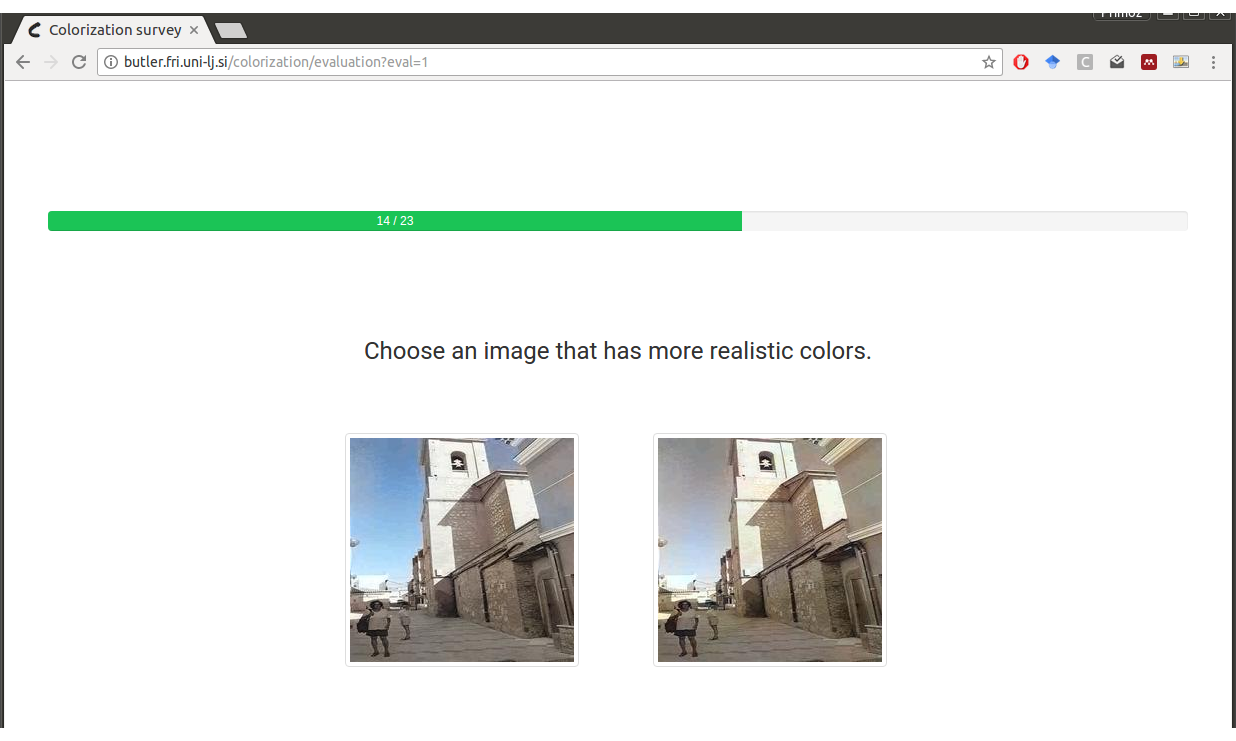
\includegraphics[width=13cm]{evaluation-1}
\end{center}
\caption{Zaslon aplikacije za evalviranje kakovosti barvanja slik s pomočjo ljudi. Anketiranec je v posameznem koraku dobil na zaslon sliko obarvano z dvema pristopoma. S klikom na sliko je ocenil, katera je bolj naravno obarvana. }
\label{im:evalvation-screen}
\end{figure}

Evalvacijo smo izvajali na skupno $100$ slikah, ki so bile izbrane naključno iz množice $10.000$ testnih slik. V evalvacijo je bilo vključenih sedem pristopov naučenih na večji učni množici, ki so našteti v poglavju \ref{ch:vecji-mnozici}.

\subsection{Aplikacija za evalvacijo}

Aplikacija za ocenjevanje je bila implementirana z ogrodjem Django\footnote{https://djangoproject.com} in je vsebovala štiri prikaze. Prvi je bil zaslon s kratkimi navodili za uporabnika. Sledil je zaslon, ki je bil namenjen kratkemu opisu poteka evalvacije, s tem smo poskrbeli, da uporabnik na prvem zaslonu ni dobil preveč informacij. Sledilo je $23$ ponovitev tretjega zaslona na katerem je potekala evalvacija in je prikazan na sliki \ref{im:evalvation-screen}. Na koncu je sledil zaslon z zahvalo in povabilom na ponovno evalvacijo. V primeru, da se je uporabnik odločil za ponovno evalvacijo, smo poskrbeli, da je vedno dobil nove slike, ki jih prej še ni videl. V primeru, da je ocenil že vse slike, mu je bila nadaljnja evalvacija onemogočena. Izvorna koda aplikacije je objavljena na GitHub repozitoriju PrimozGodec/EvaluationApp\footnote{https://github.com/PrimozGodec/EvaluationApp}.

\subsection{Statistika}

Anketiranje je potekalo v dneh od $25.$ do vključno $27.$ julija $2017$. Anketirance smo pridobili z objavo na socialnih omrežjih Facebook in LinkedIn. V anketi smo zbrali odzive $1010$ ljudi. 

Ljudje so v povprečju ocenili $21,49$ slik, če iz statistke izključimo dve testni slike, ki sta bili namenjeni privajanju na način evalvacije. Večina ljudi, kar $838$, je izpolnila anketo samo enkrat, $90$ ljudi se je odločilo za vsaj eno ponovno evalvacijo, $82$ ljudi pa je anketo zapustilo predčasno in so evalvirali manj kot $21$ slik. Zbrani podatki v obliki \textit{json} datoteke so objavljeni na GitHub repozitoriju PrimozGodec/EvaluationApp\footnote{https://github.com/PrimozGodec/EvaluationApp}.




%----------------------------------------------------------------
% Poglavje (Chapter) 5: Rezulatati in diskusija
%----------------------------------------------------------------

\chapter{Rezultati in diskusija}
\label{ch:rezultati}

V tem poglavju predstavljamo natančnosti pristopov naučenih na manjši množici in jih med seboj primerjamo. Pogledali si bomo primerjavo pristopov naučenih na večji učni množici in primerjali pristope pri barvanju večjih slik od tistih, na katerih so bili pristopi naučeni.

\section[Primerjava pristopov na manjši učni množici]{Primerjava pristopov na manjši\\ učni množici}
\label{ch:prim-manjsa}

Tabela \ref{tab:napake-100} prikazuje natančnost pristopov na testni množici slik. Izkaže se, da se na manjši množici najbolje obnese pristop Iizuka in sod., ki je glede na napako RMSE za $0,066$ boljši od našega pristopa z regresijo na celih slikah. Ostali pristopi razviti s strani drugih avtorjev se na tej množici obnesejo slabše od večine naših pristopov. 

Izkazalo se je tudi, da se na tej množici, glede na napako, regresijski pristopi obnesejo bolje kot pristopi s klasifikacijo. Pristop regresija po delih se s klasifikacijo brez uteži z arhitekturo D+G glede na RMSE razlikuje skoraj za $2$. Omenjena pristopa imata enako arhitekturo mreže. Med pristopi z regresijo je opaziti boljše rezultate pri tistih, ki barvajo celotno sliko na enkrat. Opazimo lahko tudi, da globalna mreža prinese izboljšave glede na RMSE nekje od  $0,3$ do $0,4$. Pri klasifikacijskih pristopih se je izkazalo, da arhitektura S+G deluje bolje pri tej učni množici. Izkaže se tudi, da uteži v cenilni funkciji ne prinesejo izboljšave v natančnosti.

\begin{table}[hbt]
\caption{Tabela prikazuje napake izračunane na testni množici podatkov. Za vsakega od pristopov smo izračunali napaki opisani v poglavju \ref{ch:napake}. V zgornjem delu tabele so prikazane napake na pristopih iz sorodnih del, v vmesnem napake na pristopih z regresijo in v spodnjem delu tabele napake na pristopih s klasifikacijo.}
\begin{center}
    \begin{tabular}{lccc}
    	\hline
        Pristop & RMSE & PSNR \\
        \hline
        Zhang in sod. & 15,004 & 22,252 \\
        Iizuka in sod. & 12,941 & 23,439 \\
        Dahl & 13,936 & 22,551 \\
        \hline
        Reg. po delih & 13,216 & 23,199 \\
        \hspace{0.5em} - brez softmax & 13,206 & 23,183 \\
        \hspace{0.5em} - brez globalne mreže & 13,767 & 22,840 \\
        Reg. celotna slika & 13,007 & 23,434 \\
        \hspace{0.5em} - brez globalne mreže & 13,334 & 23,068 \\
        Reg. celotna slika VGG & 13,387 & 23,131 \\
        \hline
        Klas. brez uteži - S+G & 14,336 & 22,738 \\
        Klas. brez uteži - D+G & 15,086 & 22,380 \\
        Klas. z utežmi - D+G & 14,573 & 22,610 \\         
        Klas. z utežmi - D+G & 15,137 & 22,395 \\ 
       	\hline
    \end{tabular}
\end{center}
\label{tab:napake-100}
\end{table}

Za vsak pristop smo napake za slike iz testne zbirke spremenili v range, glede na napako RMSE na določeni sliki, ki se raztezajo od najboljše z rangom $0$, do najslabše z rangom $9.999$. Izkaže se, da rangi med pristopi močno korelirajo. To pomeni, da je natančnost barvanja slike v veliki meri odvisna od motiva na sliki, kar je bilo pričakovati.

Korelacijo med pristopi je možno videti na sliki \ref{im:ranks-between-methods}. Na sliki sta prikazana grafa, ki prikazujeta odvisnost rangov med prvim pristopom na osi $X$ in drugim pristopom na osi $Y$. Izkaže se, da je korelacijo v veliki meri prisotna pri vseh pristopih, je pa nekoliko različna glede na sorodnost pristopov. Pristopa na desni sliki, ki sta si bolj podobna glede na arhitekturo in način barvanja, imata zelo veliko korelacijo, ki je skoraj linearna funkcija. Pristopa na levi sliki, ki sta si na način napovedovanja bolj različna, prvi je regresijski in druga klasifikacijski, imata manjšo korelacijo, ki pa je še vedno prisotna. Še vedno so točke razporejene okoli premice, ki razpolavlja kvadrant grafa, vendar je odstopanj več. Podobne slike dobimo tudi pri primerjavi ostalih pristopov. 

\begin{figure}[htb]
\begin{center}
\centering
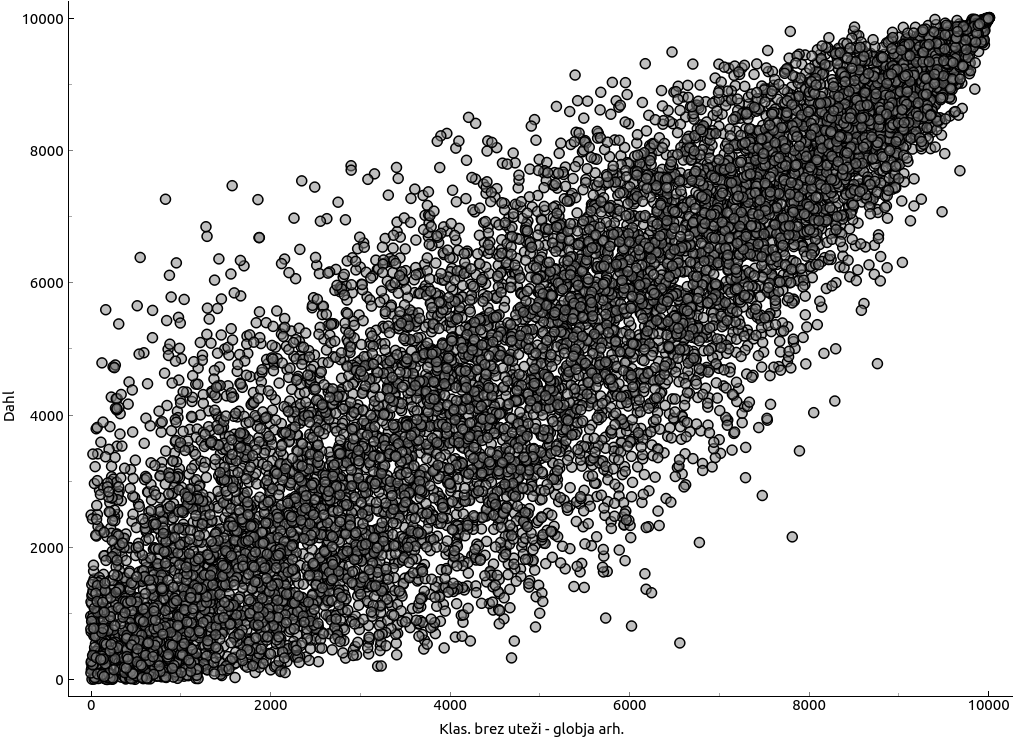
\includegraphics[width=6cm]{ranks_dahl_arh2-1}
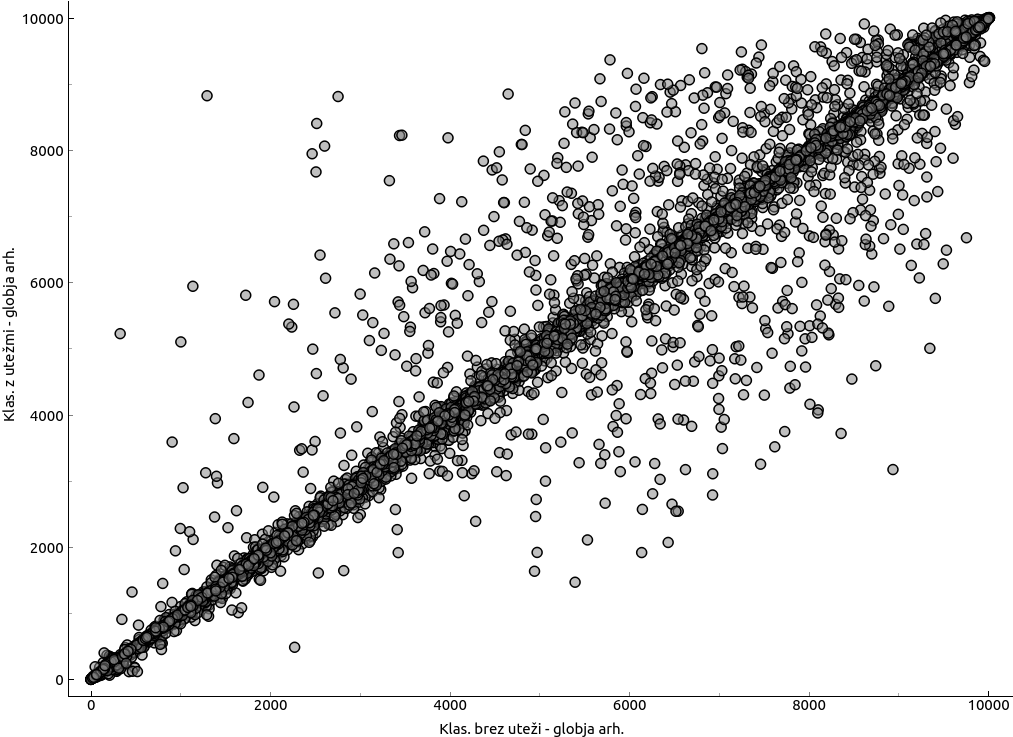
\includegraphics[width=6cm]{rank_arh2_arh2-1}
\end{center}
\caption{Grafa prikazujta rangiranje slik glede na napako RMSE pri dveh različnih pristopih. $X$ os predstavlja rang pri prvem pristopu, $Y$ pa rang pri drugem pristopu. Prva slika prikazuje primerjave rangov Dahlovega pristopa in klasifikacijskega pristopa z arhitekturo D+G. Druga slika prikazuje range pri dveh klasifikacijskih pristopih z enakimi arhitekturami.}
\label{im:ranks-between-methods}
\end{figure}

Ker smo želeli podobnost pristopov med seboj primerjati v prostoru, smo izračunali Spearmanovo korelacijo rangov \cite{hauke2011comparison} za vsak par pristopov. Korelacije so številčno prikazane v tabeli \ref{tab:spearman} v prilogi. Za izris podobnosti smo uporabili metodo večdimenzionalno skaliranje (ang. {\em multidimensional scaling} - MDS) \cite{Wickelmaier2003} na Spearmanivih korelacijah. Uporabili smo implementacijo v programu Orange \cite{demvsar2013orange}. 

Pristopi so glede na arhitekturo in vrsto pristopa razporejeni v prostor, ki je prikazan na sliki \ref{im:methods-mds}. Izkaže se, da se pristopi s klasifikacijo pojavijo desno spodaj v prostoru in so bolj oddaljeni od tistih z regresijo levo. Pri pristopih s klasifikacijo opazimo, da na različnost bolj vpliva vrsta arhitekture kot uporaba uteži za pogostost barve. Izkaže se, da je pristop Zhang in sod. bližje tistim z arhitekturo D+G. Glede na to, da so lastnosti teh arhitektur popolnoma drugačne, se izkaže, da na podobnost glede na napake vpliva predvsem globina arhitekture. 

Pri regresijskih pristopih lahko opazimo, da je največja razlika glede na uporabo globalne mreže. Pristopi, ki ne uporabljajo globalne mreže, so na vrhu prikaza, ostali so spodaj. Regresija na celotni sliki VGG je bližja pristopom z globalno mrežo. To gre verjetno pripisati dejstvu, da ta pristop uporablja mrežo VGG-16, ki je del globalne mreže pri ostalih pristopih, vendar ta pristop to mrežo izkorišča kot glavno. 

Čeprav je Dahlov pristop glede na arhitekturo popolnoma različen našim, se glede na napake izkaže podoben pristopom brez globalne mreže, kar še dodatno potrdi deljenje pristopov glede na prisotnost globalne mreže. Pristop Iizuka in sod. je v gruči s pristopi, ki uporabljajo globalno mrežo, saj tudi sam uporablja podoben pristop. Pri pristopih z regresijo lahko opazimo še, da sta pristopa Iizuka in sod. ter pristop z regresijo na celi sliki bolj skupaj, saj oba delujeta na celotni sliki. 

\begin{figure}[htb]
\begin{center}
\centering
\fbox{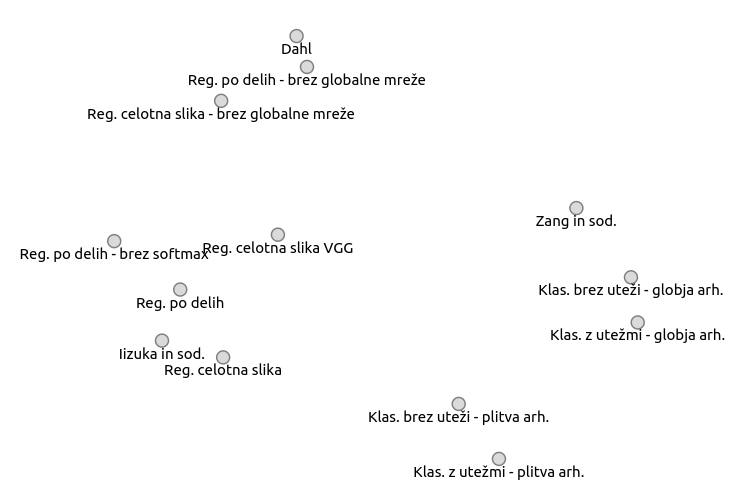
\includegraphics[width=12.5cm]{methods_mds-1}}
\end{center}
\caption{Primerjava pristopov v prostoru MDS kaže sorodnosti med pristopi glede na vrsto pristopa (klasifikacija proti regresiji), arhitekturo mreže in načinom napovedovanja (na delih ali na celih slikah). Izkaže se največja razlika med vrsto pristopa, prav tako je velika razlika med arhitekturami. Manjša je razlika med načinom napovedovanja.}
\label{im:methods-mds}
\end{figure}

Zanimalo nas je tudi katere so tiste slike, kjer eden od pristopov opravi dobro delo, ostali pa mnogo slabše in obratno. Ob pogledu na sliko \ref{im:ranks-between-methods} lahko opazimo, da so taki primeri točke, ki ležijo najbolj stran od linearne premice, zato smo te slike našli z metodo za iskanje osamelcev (ang. {\em outliers}) \cite{Ramaswamy}. 

Slike, ki najbolj izstopajo glede na napako na različnih pristopih, so prikazane kot točke v prostoru, ki ga dobimo z metodo MDS glede na napako, na sliki \ref{im:images-mds}. Ob pregledu slik se izkaže, da gre tukaj večinoma za slike, kjer je težje zaznati teksturo. Ob tem predvidevamo, da so se določeni pristopi bolje naučili ravno te teksture kot drugi pristopi. 

Ob bolj natančnem pregledu prostora smo ugotovili, da je napaka močno povezana z motivom na sliki. V prostoru so bližje skupaj slike s podobnim motivom in barvami. Na levi strani so prikazane tri slike, ki so blizu skupaj in jim je skupno to, da je na sliki morje ali nebo, ki sta oba modre barve in imata prisoten določen objekt (v našem primeru žival). Na desni strani sta dve sliki, ki se tudi ujemata glede na odtenke v sliki, čeprav je motiv popolnoma drugačen. 

\begin{figure}[htb]
\begin{center}
\centering
\fbox{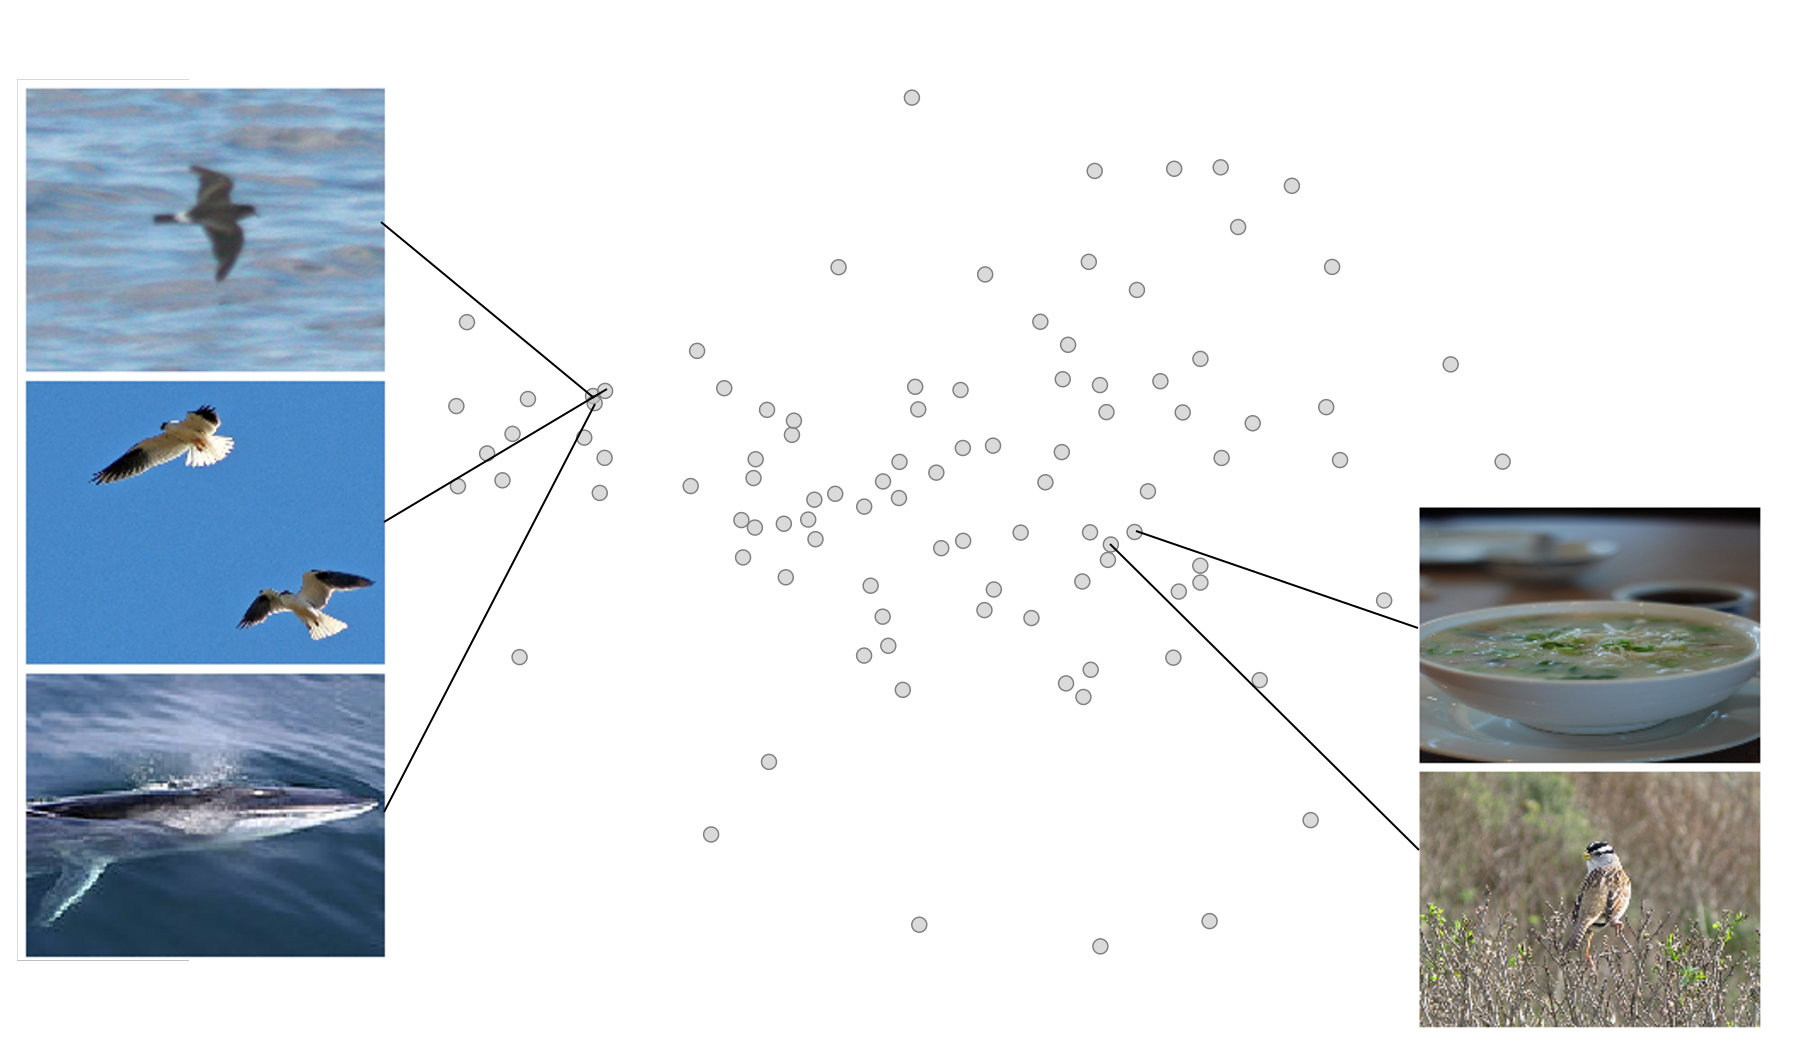
\includegraphics[width=13cm]{images_mds}}
\end{center}
\caption{Razporeditev slik v prostoru MDS, ki zajema $100$ slik, pri katerih so natančnosti najbolj različne glede na rang pri različnih pristopih. Prostor je bil izrisan glede na metodo MDS. Opazimo lahko, da so v prostoru podobne slike bližje skupaj. Dve taki podobni skupini slik sta prikazani ob robu.   }
\label{im:images-mds}
\end{figure}

Ker se ukvarjamo s slikami, dodajamo še primerjavo barvanja na slikah. Primerjave po pristopih so prikazane na sliki \ref{im:images-100-compare-reg} za regresijo in na sliki \ref{im:images-100-compare-klas} za klasifikacijo. Slike smo izbrali tako, da prva dva stolpca prikazujeta dve slike iz množice dvajset najbolje obarvanih s strani vseh pristopov, tretji in četrti stolpec prikazujeta slike, ki so se bile različno dobro obarvane s strani različnih pristopov. Ti sliki sta izbrani izmed točk v prostoru na sliki \ref{im:images-mds}. Zadnja dva stolpca prikazujeta slike, ki so bile v množici dvajset najslabše obarvanih s strani vseh algoritmov. 

Opazimo lahko, da sliki v prvih dveh stolpcih spadata v skupino najbolje obarvanih slik zato, ker imajo že originalne slike prisotne zelo malo barve. Pristopi, posebej regresijski, ki običajno obarvajo z bolj nenasičenimi (bledimi) barvami, so se zato zelo približali originalni sliki, čeprav barvanje v več primerih ni ravno najboljše. Pri drugem in tretjem stolpcu so se nekateri pristopi dobro približali pravi barvi, drugi pa so obarvali popolnoma narobe. Sliki iz zadnjih dveh stolpcev sta bili glede na napako v množici najslabše obarvanih slik zato, ker imajo originalne slike zelo močne odtenke, katerim se pristopi niso približali. Kljub temu so nekatera barvanja dovolj naravna v primeru, da jih ne primerjamo z originalno sliko.

V primerjavi s pristopi iz sorodnih del pričakovano opazimo, da najboljše barva pristop Iizuka in sod., ki je imel tudi najmanjšo napako. Zang in sod. se na določenih delih obnese dobro, vendar so slike zelo lisaste in nepopolno obarvane, medtem ko so pri pristopu Dahl odtenki zelo rjavi, čeprav vmes lahko opazimo nekaj pravih barv.

Pri primerjavi regresijskih pristopov lahko opazimo, da je po pričakovanjih najboljše barvanje s strani regresije na celotni sliki z globalno mrežo, čeprav regresija na delih slik ne zaostaja dosti. Opazimo lahko tudi pomen in izboljšavo z uporabo globalne mreže. Enaki pristopi brez globalne mreže so obarvali bolj nenatančno, nenaravno, prisotnih je tudi več rjavih odtenkov. 

Pri klasifikacijskih pristopih opazimo, da pristopi s arhitekturo S+G dajejo boljše rezultate kot tisti z D+G, kjer barvanja skorajda ni. Pri primerjavi z utežmi in brez lahko zaznamo, da pristop z utežmi barva z močnejšimi odtenki kot tisti brez, kar je bilo za pričakovati, saj je namen uteži zmanjšati izbor šibkejših odtenkov, ki imajo $a*$ in $b*$ vrednost bližje nič. Pristopi so nagnjeni k izbiri nežnejših odtenkov, ker se bolj pogosto pojavljajo v slikah. Kljub barvanju z močnejši odtenki barv in s tem približevanju realni barvi, je na pogled barvanje brez uteži bolj naravno, saj je opaziti manj napak v barvanju. Za primer lahko vzamemo sliko s ptico, kjer sta les in ptica pobarvana bolj realno in letalo nima sivega pasu okoli sebe.

Iz primerjave slik lahko opazimo, da pristopi z regresijo obarvajo bolje in bolj naravno kot pristopi s klasifikacijo, čeprav je nekaj izjem pri barvanju neba in praproti. Izkaže se tudi, da barvanje z regresijo večkrat obarva z bolj rjavimi odtenki, kar pri klasifikacijskih pristopih ni zaznati. Tam je bolj pogosto, da slika ni obarvana. 

% \afterpage{\clearpage}
\begin{figure}[htbp]
\begin{center}
\centering
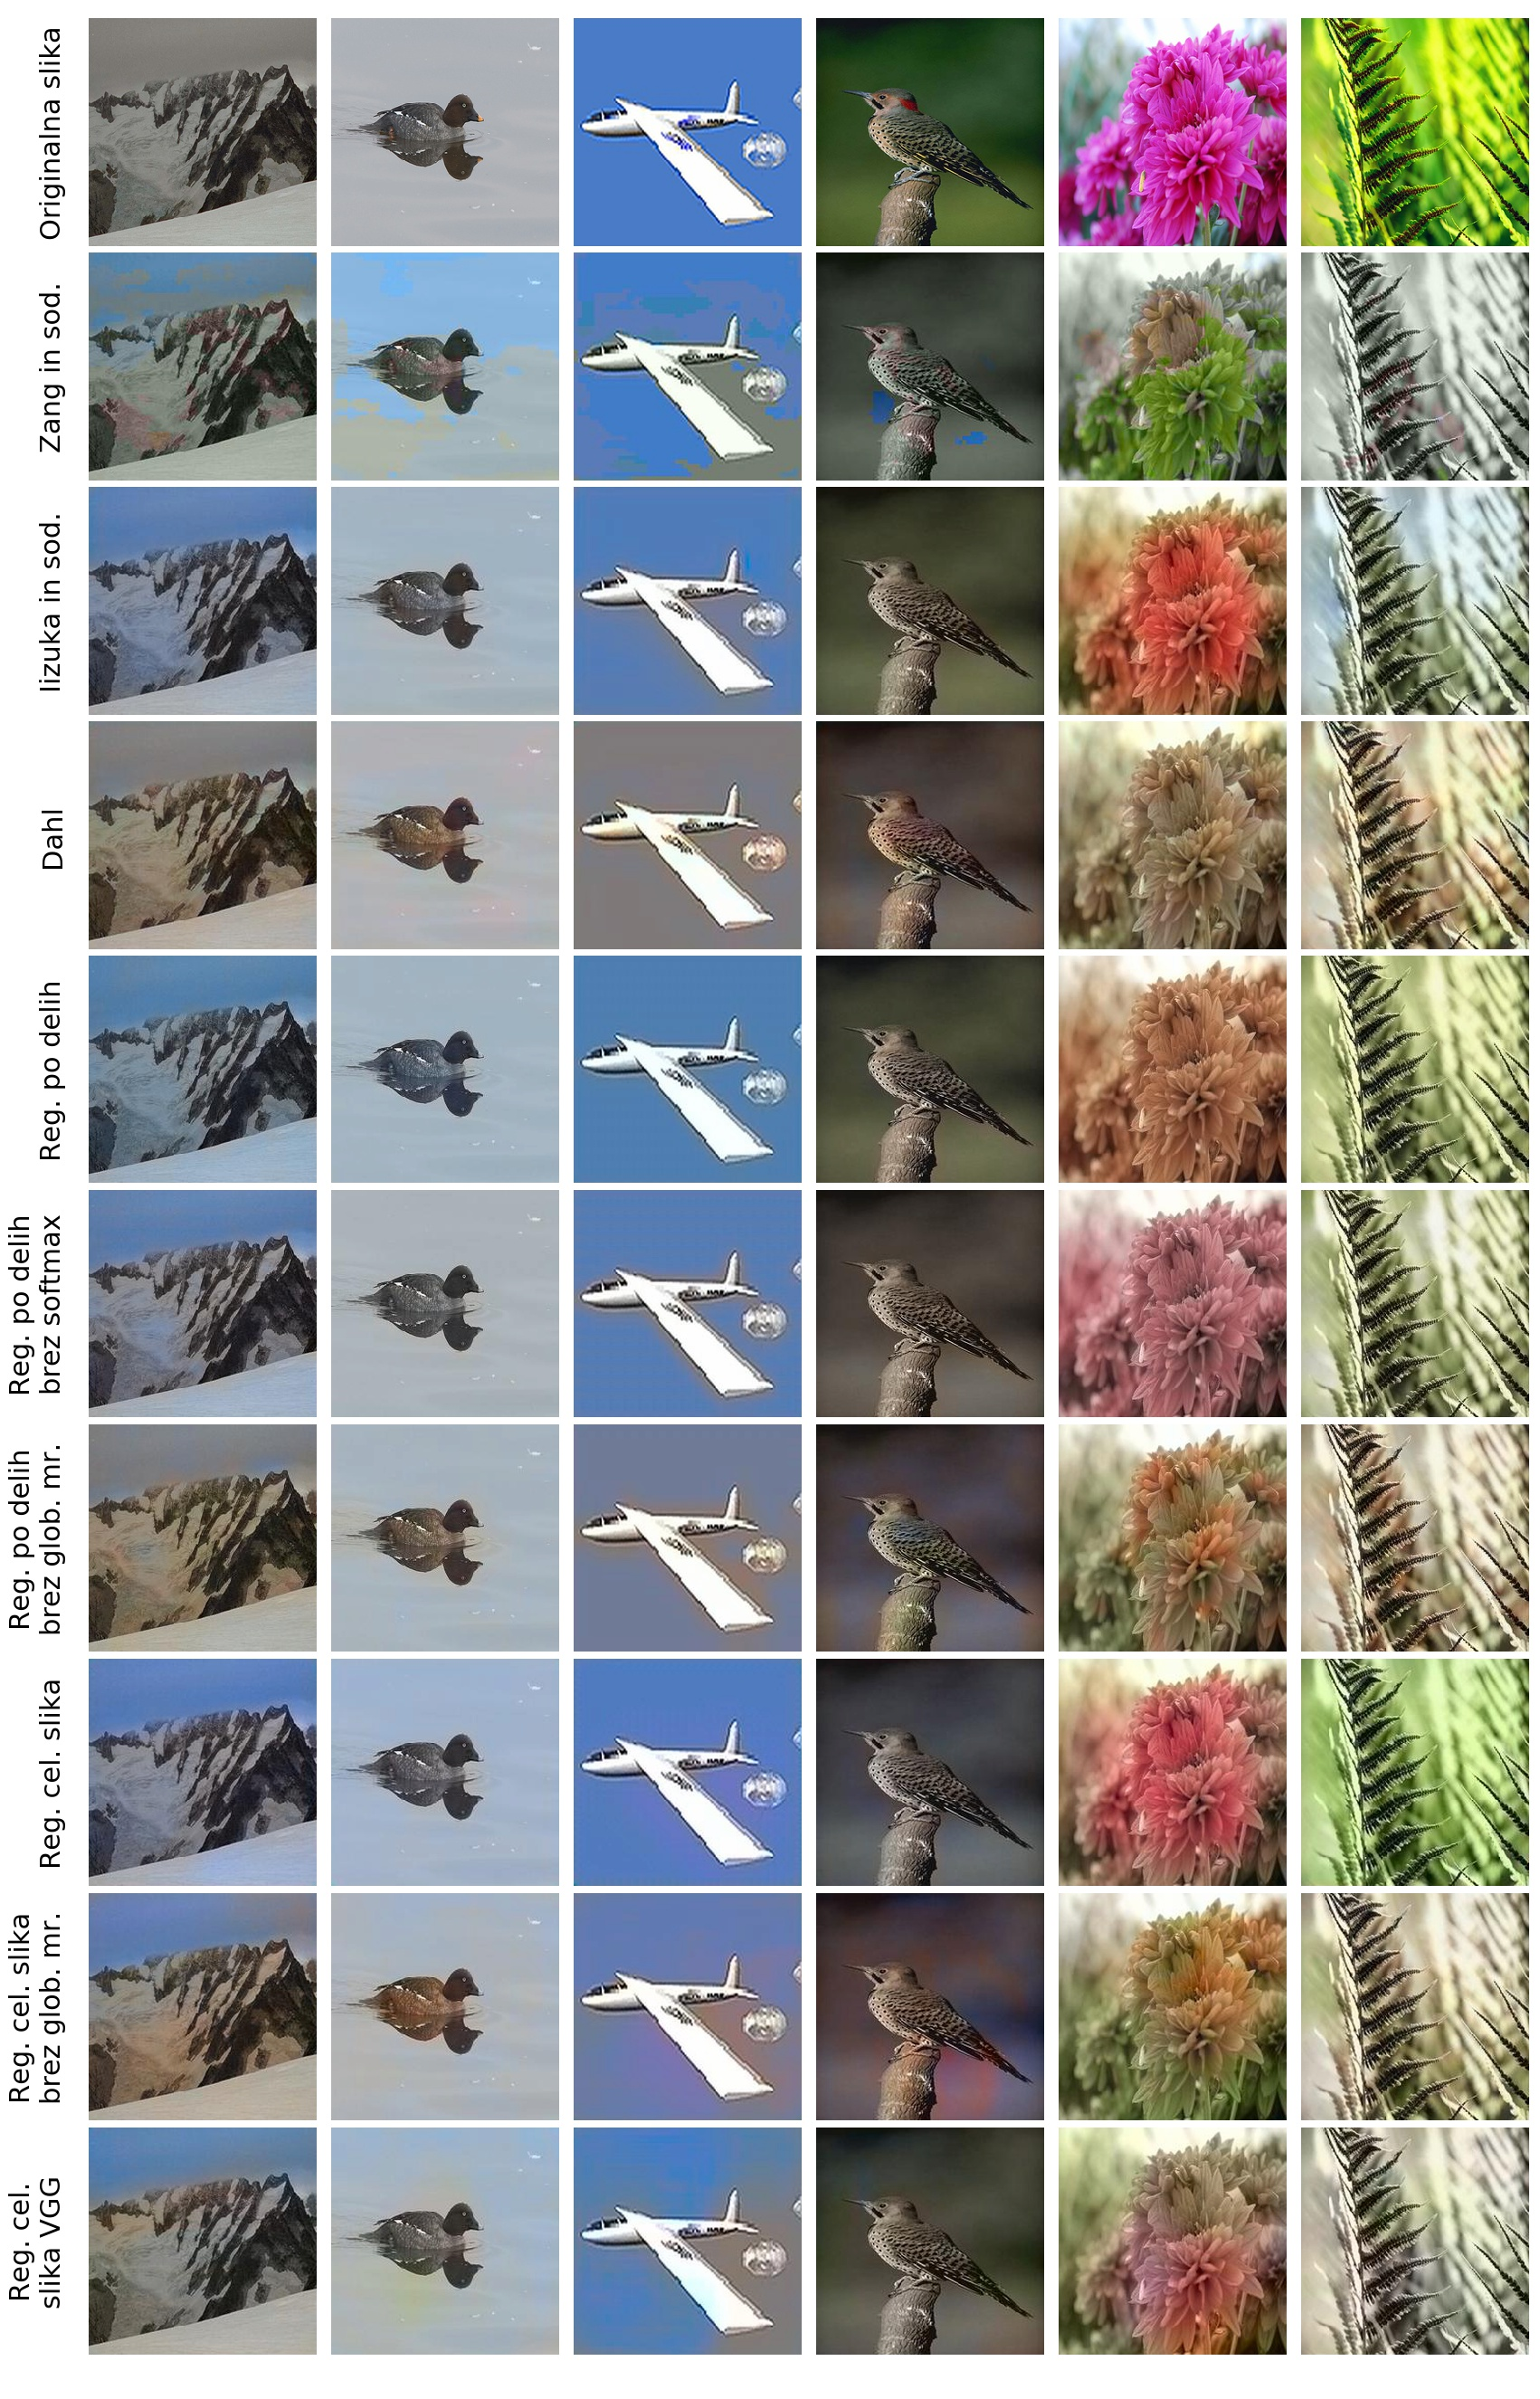
\includegraphics[width=11.3cm]{images-methods-comparison-100-reg-1}
\end{center}
\caption{Slike iz testne množice, ki so bile obarvane z regresijskimi pristopi opisanimi v tem delu in pristopi iz sorodnih del. Vsaka vrstica prikazuje drug pristop, prva vrstica prikazuje originalno sliko.}
\label{im:images-100-compare-reg}
\end{figure}

% \afterpage{\clearpage}
\begin{figure}[htbp]
\begin{center}
\centering
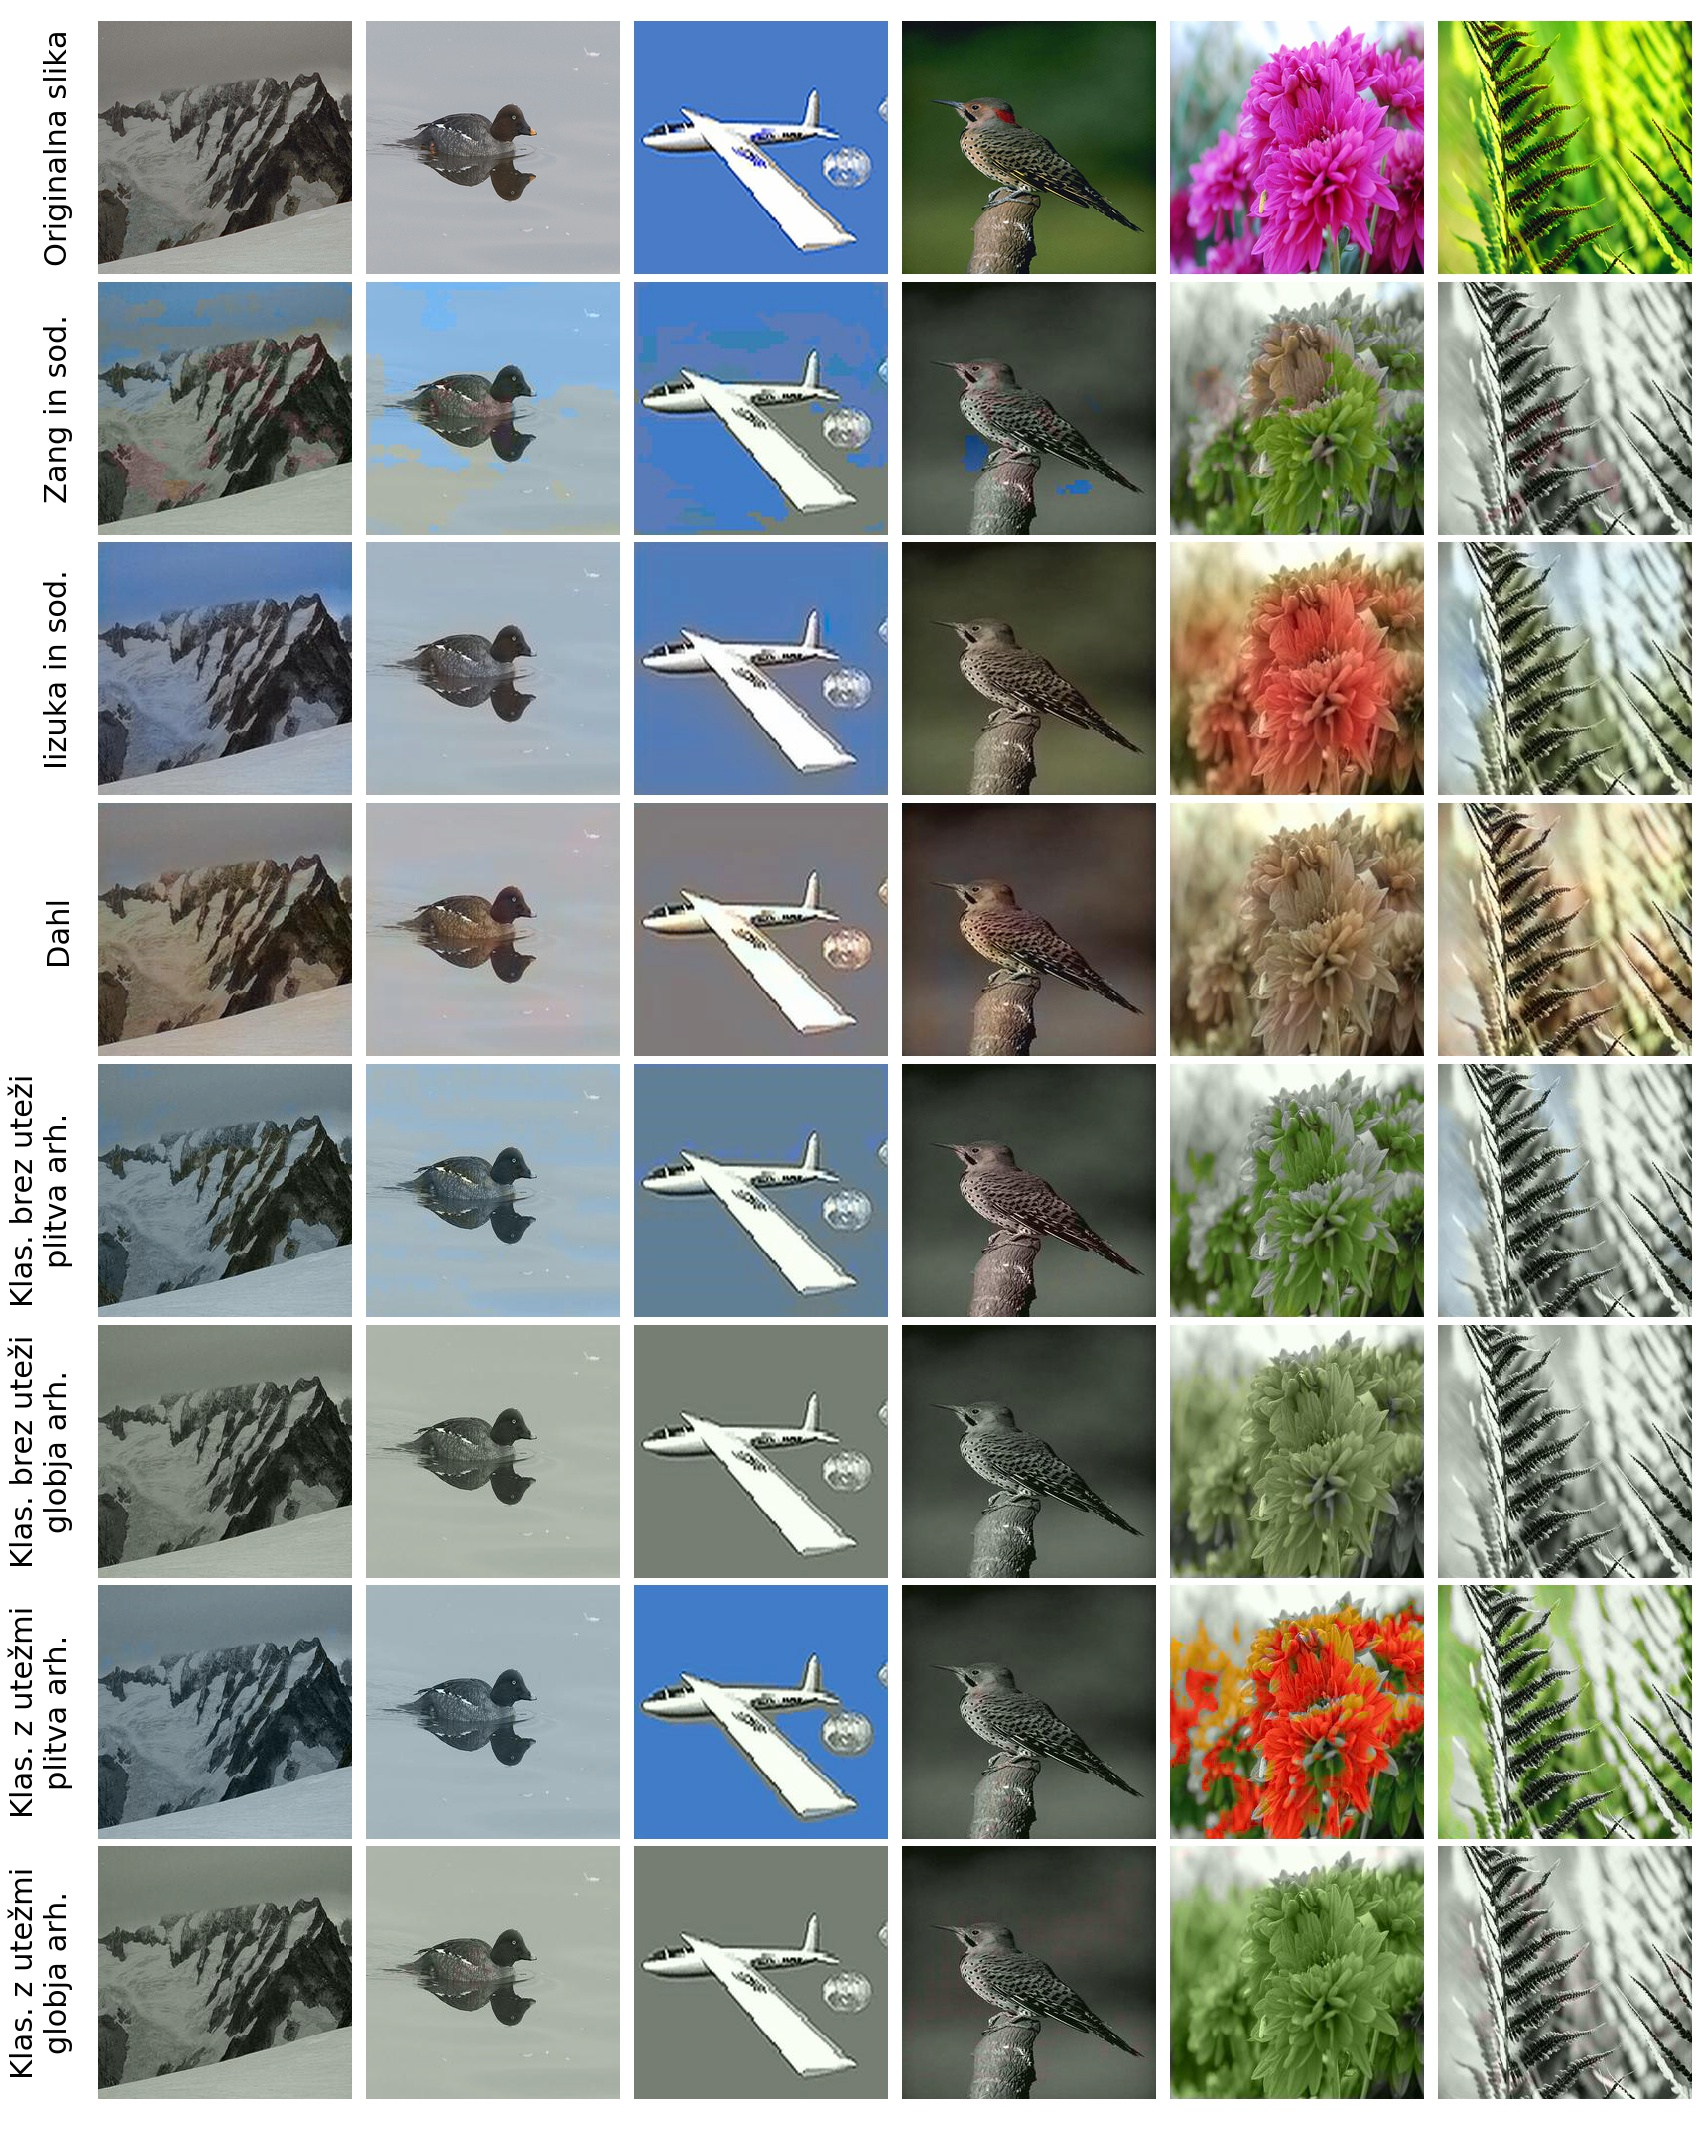
\includegraphics[width=11.3cm]{images-methods-comparison-100-klas-1}
\end{center}
\caption{Slike iz testne množice, ki so bile obarvane s klasifikacijskimi pristopi opisanimi v tem delu in pristopi iz sorodnih del. Vsaka vrstica prikazuje drug pristop, prva vrstica prikazuje originalno sliko. }
\label{im:images-100-compare-klas}
\end{figure}

% here
\section[Primerjava pristopov na večji učni množici]{Primerjava pristopov na večji \\ učni množici}
\label{ch:rez-vecji}

V tabeli \ref{tab:napake-full} so prikazane napake pristopov, ki so naučeni na večji učni množici. Opazimo, da je razmerje med pristopi ostalo nespremenjeno glede na rezultate v poglavju \ref{ch:prim-manjsa}. Prav pri vseh pristopih se  je po pričakovanjih izboljšala natančnost barvanja. Kot lahko opazimo, če rezultate primerjamo s tistimi v tabeli \ref{tab:napake-100}, smo največjo izboljšavo pridobili pri pristopih Iizuka in sod. in klasifikacija z utežmi s arhitekturo S+G. 

\begin{table}[hbt]
\caption{Tabela prikazuje napake izbranih pristopov izračunane na testni množici podatkov. Za vsakega od pristopov smo izračunali dve napaki opisani v poglavju \ref{ch:napake}. V zgornjem delu tabele so prikazane napake na pristopih iz sorodnih del, v vmesnem napake na pristopih z regresijo in v spodnjem delu tabele napake na pristopih s klasifikacijo.}
\begin{center}
    \begin{tabular}{lccc}
    	\hline
        Pristop & RMSE & PSNR \\
        \hline
        Iizuka in sod. & 12,252 & 23,831 \\
        Dahl & 13,745 & 22,827 \\
        \hline
        Reg. po delih & 12,960 & 23,363 \\
        Reg. celotna slika & 12,368 & 23,829 \\
        Reg. celotna slika VGG & 12,976 & 23,398 \\
        \hline
        Klas. brez uteži - S+G & 14,015 & 22,909 \\
        Klas. z utežmi - S+G & 14,326 & 22,717 \\         
       	\hline
    \end{tabular}
\end{center}
\label{tab:napake-full}
\end{table}

Slika \ref{im:full-learning} prikazuje napredovanje barvanja po prvih desetih korakih učenja. Korak predstavlja učenje na sklopu $50.000$ slik. Deset korakov smo izbrali, ker je tu viden največji napredek. Izkaže se, da je pri vseh pristopih največja razlika narejena že v prvem koraku, v nadaljnjih pa se dogajajo spremembe, ki večinoma barvanje naredijo bolj realno. 

\begin{figure}[htbp]
\begin{center}
\centering
\includegraphics[width=10.6cm]{n00443692_1173-learning-1}
\end{center}
\caption{Napredovanje barvanja po prvih desetih korakih učenja pri različnih prestopih. Stolpec predstavlja pristop, vsaka vrstica pa posamezen korak. }
\label{im:full-learning}
\end{figure}

Za konec predstavitve smo izbrali še nekaj slik, ki so bile dobro obarvane pri skoraj vseh pristopih in nekaj slik katerih barvanje je bilo slabo ali delno slabo v vseh primerih.

Dobro obarvane slike so prikazane na sliki \ref{im:images-full-compare-1}. Te slike so v večini slike narave in tiste z zelo pogostimi motivi, ki imajo enako barvo v vseh primerih. Na primer rdeč opečnat zid na zadnji sliki je zelo dobro obarvan, saj je vedno enake barve, prav tako rdeč paradižnik. Opazimo lahko, da pristopi Iizuka in sod ter regresija po delih in regresija na celotni sliki v večji meri barvajo bolj natančno. Izkaže se, da pristopa Iizuka in sod. in regresija na celih slikah nimata bistvenih razlik v kakovosti barvanja pri slikah, ki sodijo v množico dobro obarvanih slik. Iz tega lahko sklepamo, da se pristop regresija na celih slikah izkaže slabše od pristopa Iizuka in sod. na slikah, ki sodijo v množico slabše obarvanih slik. Regresija po delih nekoliko zaostaja, vendar je barvanje še vedno realno. Klasifikacijska pristopa se izkažeta za manj natančna, vidi pa se, da pristop z utežmi poskuša barvati z močnejšimi odtenki. To se najbolje opazi pri paradižniku, ki je še najbolje obarvan prav s tem pristopom. Izkaže se, da so največje razlike pri barvanju pri podvodnih slikah, mogoče bi to lahko pripisali manj očitnim teksturam v sliki. Presenečeni smo nad kvaliteto barvanja košarkarske žoge, saj nismo pričakovali, da bo tako dobro obarvana. Očitno je v učni množici več primerov takšnih žog. 

%\afterpage{\clearpage}
\begin{figure}[htbp]
\begin{center}
\centering
\includegraphics[width=11.5cm]{images-methods-comparison-full-4}
\end{center}
\caption{Slike iz testne množice, barvanje katerih se je izkazalo za dobro. Vsak stolpec predstavlja enega od pristopov opisanih v delu. }
\label{im:images-full-compare-1}
\end{figure}

Slika \ref{im:images-full-compare-2} prikazuje sike, ki so obarvane slabše. Slike so obarvane slabo iz več razlogov. Pri večini gre za problem pri predmetih z neenoličnimi barvami. V tem primeru nekateri pristopi obarvajo naravno, vendar drugače kot je v originalu, s čimer ni nič narobe, nekateri pa obarvajo popolnoma narobe. Seveda je vse odvisno od motiva. Šopek rož je na primer praktično pri vseh regresijskih pristopih obarvan naravno. Tudi jakna na sliki je v nekaterih primerih obarvana naravno. Medtem ko notranjost prostorov in zunanjost hiš ni prepričljivo obarvana. V nekaterih primerih pride do napake, ko določen predmet ali žival dobi barvo okolice. To se večkrat zgodi pri pristopih po delih vendar ni zelo običajno. Sklepamo lahko, da se ti pristopi občasno preveč opirajo na globalno mrežo. Veliko slik je obarvanih z premalo nasičenimi barvami. To se dostikrat zgodi pri predmetih, ki nimajo enolične barve. Na primer rdeč avto kaže zametke rdečih odtenkov, ki pa niso ravno prepričljivi. Pri sliki v drugi vrsti so skalne stene zelo močno rdečih odtenkov. Ker mreža večkrat vidi primer sivih skal, je tudi tukaj barvanje bolj sivo kot rdeče. 

Kot smo ugotovili že v poglavju \ref{ch:prim-manjsa}, lahko tudi na primerih slik zaključimo, da je kvaliteta barvanja v veliki meri odvisna od motiva na sliki. Večino dobro obarvanih slik je pri vseh pristopih obarvano pristopu primerno, medtem kot tiste slabo obarvane, večinoma slabo obarvane pri vseh pristopih. Barvanje se redko približa kvaliteti originalne slike, vendar v večini primerov uporabi prave barve, odtenki pa niso vedno najbolj prepričljivi.

\begin{figure}[htbp]
\begin{center}
\centering
\includegraphics[width=11.7cm]{images-methods-comparison-full-3}
\end{center}
\caption{Slike iz testne množice barvanje katerih se je izkazalo za slabše. Vsak stolpec predstavlja enega od pristopov opisanih v delu. }
\label{im:images-full-compare-2}
\end{figure}


\section[Primerjava pristopov glede na realističnost barvanja]{Primerjava pristopov glede na \\ realističnost barvanja}

Za primerjavo pristopov smo zgradili Bradley–Terry model \cite{hunter2004mm}. Parametre smo ocenili z metodo največjega vrjetja (ang. {\em  maximum likelihood}). Model je zgrajen tako, da nam je v pomoč pri rangiranju podatkov pridobljenih v medsebojni primerjavi parov. Pri katerem ni nujno, da so primerjave popolne in enako pogoste za pare.

Model je bil zgrajen na podlagi primerjav prikazanih v tabeli \ref{tab:rez-survey} v prilogi. Izračunana sta bila parametra $\gamma_i$ in $\beta_i$, ki sta si v razmerju $\gamma_i = e^{\beta_i}$, kjer je $i$ zaporedna številka pristopa. Večja vrednost parametra pomeni pristop, ki se je bolje izkazal glede na evalvacijo. Parametri so prikazani v tabeli \ref{tab:rang-survey}.

\begin{table}[hbt]
\caption{Vrednosti parametrov Bradley-Terry modela za pristope, ki jih primerjamo. Večja vrednost pomeni, da se je pristop bolje izkazal pri ocenjevanju.}
\begin{center}
    \begin{tabular}{lccc}
    	\hline
        Pristop & $\gamma_i$ & $\beta_i$ \\
        \hline
        Iizuka in sod. & 0,277 & -1,28 \\
        Dahl & 0,125 & -2,08 \\
        \hline
        Reg. po delih & 0,106 & -2,25 \\
        Reg. celotna slika & 0,189 & -1,67 \\
        Reg. celotna slika VGG & 0,130 & -2,04 \\
        \hline
        Klas. brez uteži - S+G & 0,098 & -2,32 \\
        Klas. z utežmi - S+G & 0,076 & -2,58 \\         
       	\hline
    \end{tabular}
\end{center}
\label{tab:rang-survey}
\end{table}
 
Če rezultate primerjamo s tistimi v poglavju \ref{ch:rez-vecji}, kjer smo pristope primerjali glede na izračunano napako, vidimo določene podobnosti in tudi razlike. Najbolje se je enako kot pri napaki s primerjavo z originalno sliko izkazal pristop Iizuka in sod. Zaostaja naš pristop z regresijo na celih slikah, do spremembe pa je prišlo pri pristopu z regresijo na celih slikah z mrežo VGG, ki se je glede na oceno ljudi izkazal za boljšega od regresije po delih. Enako kot prej je pristop, ki ga je razvil Dalh, boljši od klasifikacijskih, ki se tudi v primeru evalvacije s pomočjo ljudi izkažeta za slabša. 


\section{Barvanje večjih slik}

Tabela \ref{tab:vecjih} prikazuje napake pri dveh velikostih slik na dveh pristopih. Ena velikost je velikost na kateri je bila mreža naučena, druga pa je štirikratna velikost slik v višino in širino. Izkaže se, da ima pristop regresija po delih z globalno mrežo zelo majhno razliko v napaki, pri barvanju slik večjih velikosti glede na napako na osnovni velikosti, medtem je ta razlika pri pristopu Iizuka in sod. merjena v RMSE kar $6,18$. 

\begin{table}[htb]
\caption{Primerjava napak pristopov Iizuka in sod. ter regresija po delih z globalno mrežo pri barvanju dveh velikosti slik. $224 \times 224$ je velikost na kateri je bila mreža naučena, druga velikost je uporabljena za testiranje razlike v barvanju večjih slik. Za računaje napake so uporabljene metrike opisane v poglavju \ref{ch:napake}.}
\begin{center}
\begin{tabular}{lccc}
\hline
Pristop & Velikost slik & RMSE & PSNR \\
\hline
\multirow{2}{*}{Iizuka in sod.} & 224 & 10,018 & 24,750 \\
 								& 896 & 16,136 & 20,906 \\
\hline
\multirow{2}{*}{Reg. po delih} & 224 & 9,892 & 24,700 \\
 								& 896 & 10,096 & 24,523 \\
\hline
\end{tabular}
\end{center}
\label{tab:vecjih}
\end{table}


\section{Barvanje starih slik}

Glavna motivacija magistrskega dela je bilo razviti pristop za barvanje črno-belih slik z namenom, da obarvamo stare črno-bele slike. 
Zato smo pristop uporabili na množici zgodovinskih slik. Za barvanje zgodovinskih slik smo uporabili pristop, ki se je najbolje obnesel, to je regresija na celotni sliki. 

Rezultati barvanja zgodovinskih slik so prikazani na sliki \ref{im:history}. Iz rezultatov lahko opazimo dobro barvanje objektov z enolično določeno barvo. Nekaj več napak zaradi pomanjkljive kvalitete slik lahko opazimo na nekaterih delih. Tam, kjer je barvna neenolična, je prisotnih več rjavih odtenkov, česar smo že vajeni iz prejšnjih primerov. Slike niso enake tistim, ki bi bile zajete z barvnim fotoaparatom, če bi obstajal, ampak so bolj nežnih in nenasičenih odtenkov. V večini primerov so barve smiselne in doprinesejo k živahnosti fotografije. 

\begin{figure}[htbp]
\begin{center}
\centering
\includegraphics[width=11cm]{old-1}
\end{center}
\caption{Pari črno-belih zgodovinskih slik in obarvanih slik. Slike so pridobljene iz spletnih podatkovnih zbirk navedenih v poglavju \ref{ch:podatki}.}
\label{im:history}
\end{figure}

\subsection{Konvergenca nevronske mreže}

Pri učenju smo beležili vrednosti cenilne funkcije po vsakem končanem prehodu čez vse podatke (ang. {\em epoch}) na učni množici in validacijskih množici. S tem smo opazovali, kdaj je določen pristop optimalno naučen. To se v našem primeru zgodi v trenutku, ko vrednost cenilne funkcije na validacijski množici prenehajo padati ali začne naraščati. V tem trenutku je naša mreža optimalno naučena, zato smo te uteži uporabili za testiranje. Grafi padanja cenilnih funkcij za vse pristope naučene na manjši učni množici so prikazani na sliki \ref{im:histograms-100}. 

%\afterpage{
\begin{figure}[p]
\begin{center}
\centering
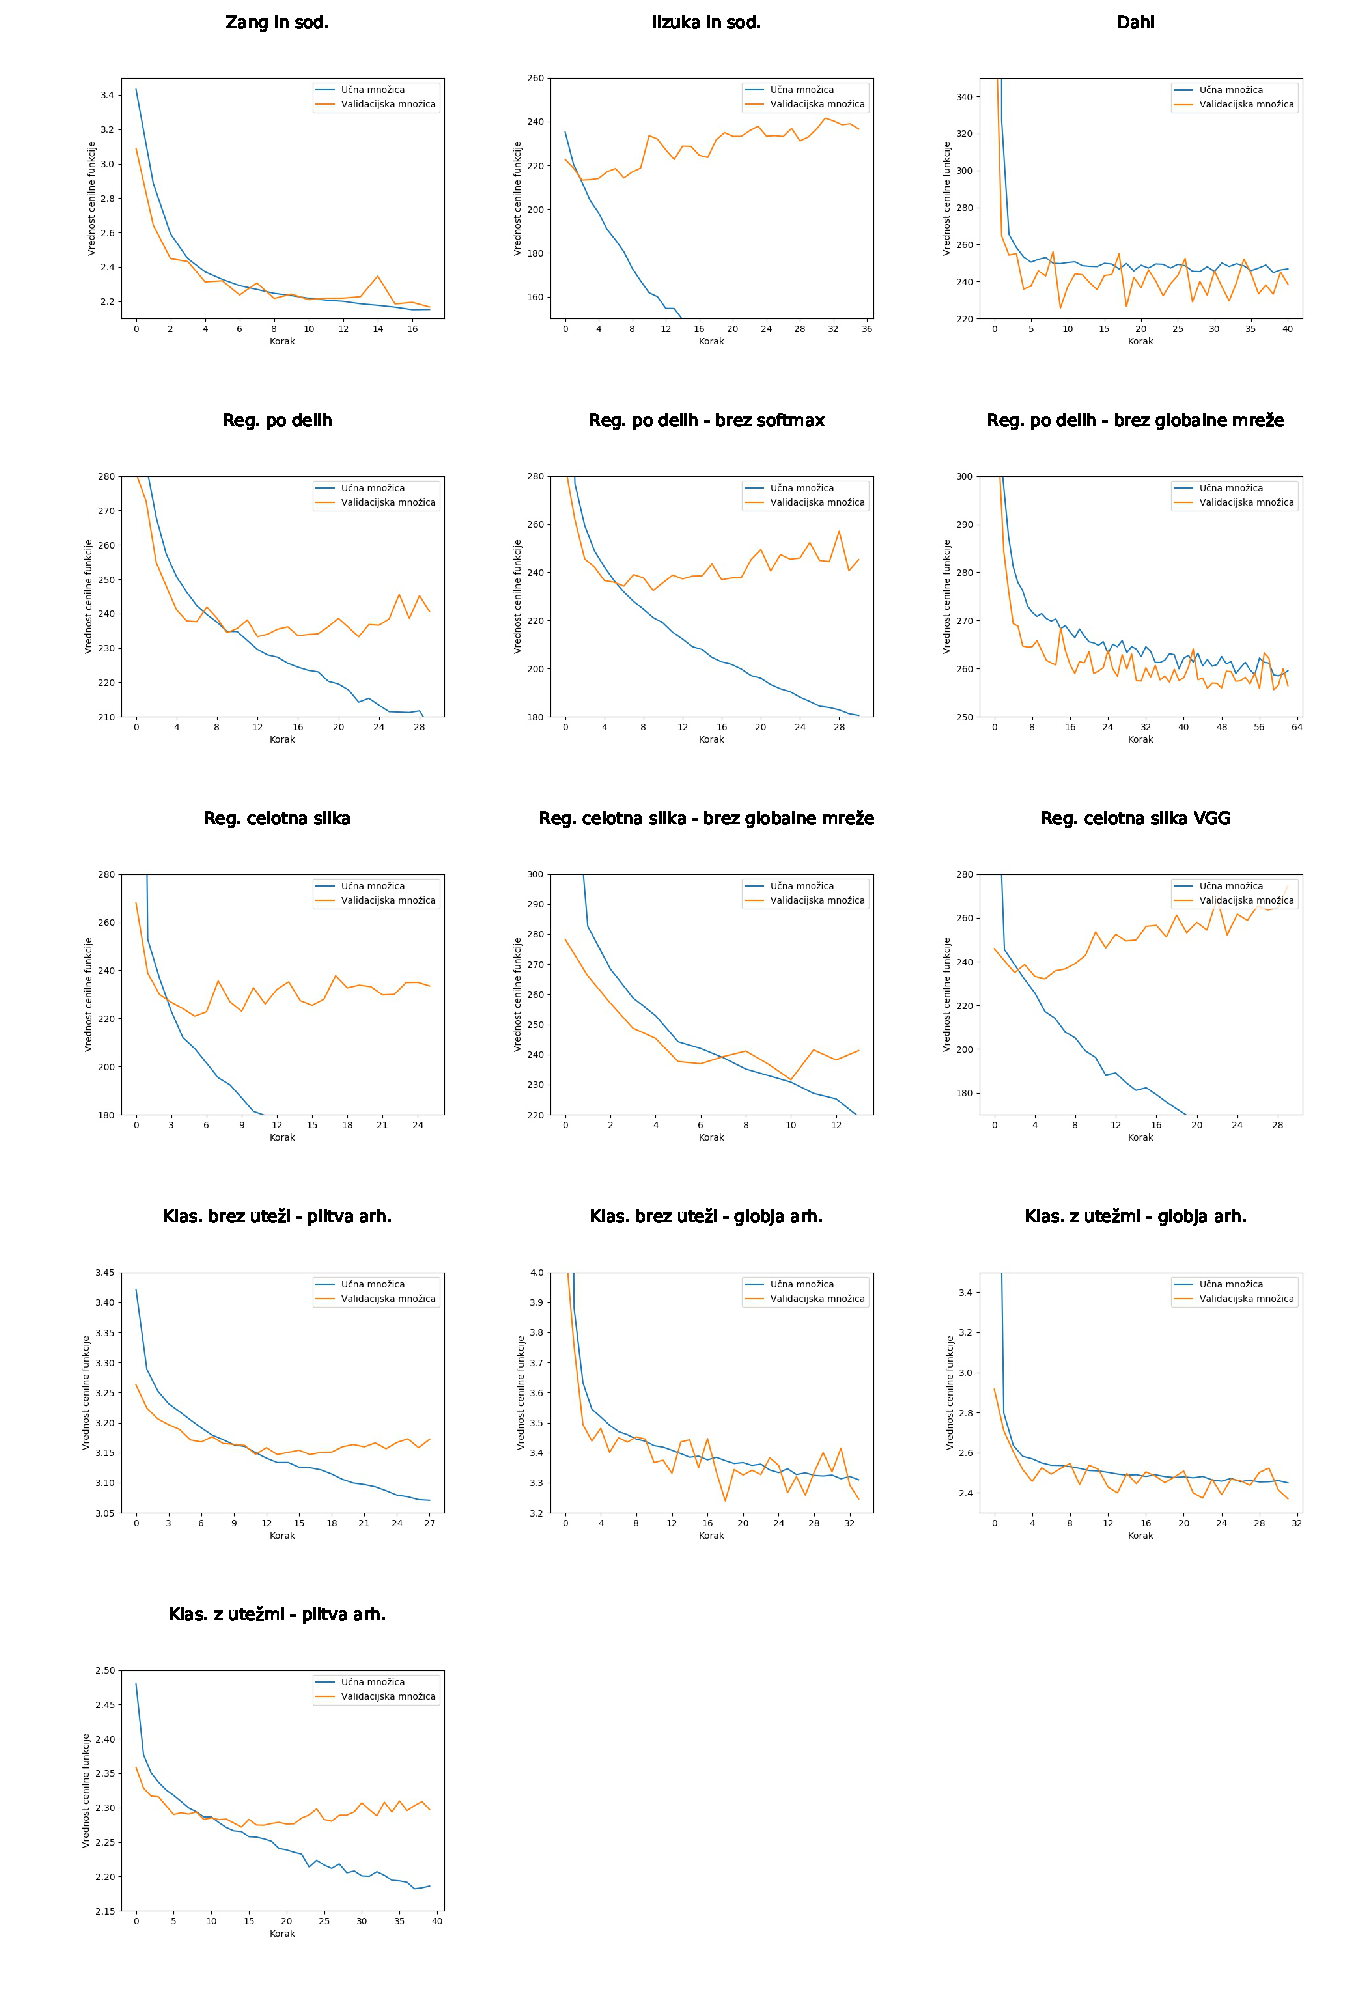
\includegraphics[width=12cm]{histograms-100-2}
\end{center}
\caption{Prikaz padanja napake modela pri učenju na manjši množici. Za vsak prehod preko vseh podatkov (ang. {\em epoch}) je prikazana vrednost cenilne funkcije na učni in validacijski množici. }
\label{im:histograms-100}
\end{figure}
%}

Enako kot v primeru na manjši učni množici smo si tudi pri večji izrisovali vrednosti cenilne funkcije na učni množici in validacijski množici. Spreminjanje teh vrednosti je prikazano na sliki \ref{im:histograms-full}. 

\begin{figure}[hbt]
\begin{center}
\centering
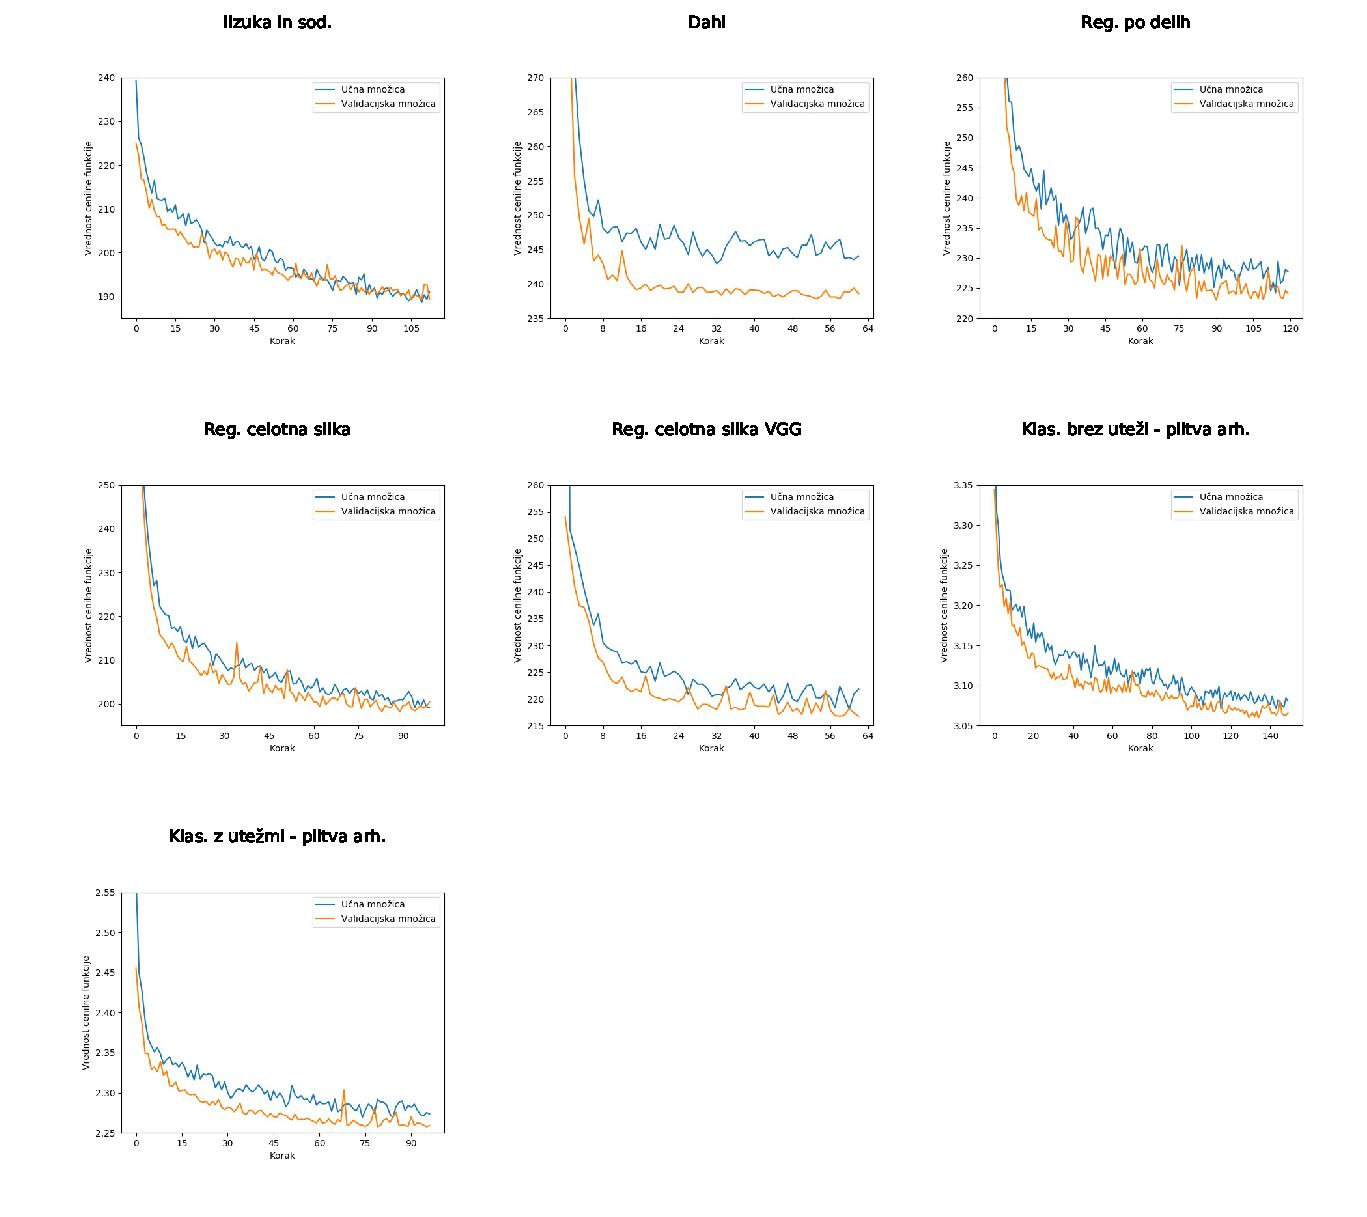
\includegraphics[width=12cm]{histograms-full-1}
\end{center}
\caption{Prikaz padanja napake modela pri učenju na večji množici. Za vsak prehod preko $50.000$ slik je prikazana vrednost cenilne funkcije na učni množici in validacijski množici. }
\label{im:histograms-full}
\end{figure}

\subsection{Pomen nivojev mreže}

Konvolucjsko nevronsko mrežo si lahko predstavljamo kot nivoje, ki poskrbijo za zajem značilk iz slike. V preteklosti so to počeli z različnimi pristopi kot so SIFT \cite{ke2004pca}, HOG \cite{ke2004pca}, SURF \cite{bay2006surf} in ostalimi. Nevronska mreža za to poskrbi sama in izlušči tiste značilke, ki so za določeno nalogo relevantne. Uporabljene značilke lahko v grobem vidimo z vizualizacijo izhodov konvolucijskih nivojev. 
 
V tem poglavju bomo pogledali, katere značilke zaznajo nivoji. V ta namen smo izrisali izhode prvih šestih konvolucijskih nivojev nevronske mreže, ki so prikazani na sliki \ref{im:layers-vis}. Vsak nivo predstavlja več slik, ki so izhodi posameznih filtrov, število slik pa je odvisno od števila filtrov. Čeprav ima mreža več nivojev, smo se odločili, da prikažemo le prvih šest, saj so ti najbolj razumljivi. Za vizualizacijo smo si izbrali pristop regresija na celotni sliki z globalno mrežo, saj je ta najbolj zgovorna za vizualizacijo.

Slike prikažejo na katere elemente se filtri v posameznem nivoju odzivajo, oziroma kaj zaznavajo. V prvem nivoju lahko opazimo, da se v večji meri osredotočajo na robove v sliki. Opazimo lahko, da se nekateri odzovejo tudi na večji del slike, kar vidimo kot nekoliko okrnjeno vhodno sliko. V drugem nivoju  opazimo že bolj osredotočene odzive. Nekateri še vedno zaznajo robove, drugi pa se že osredotočijo samo na določene dele slike, na primer vodoravne ali navpične robove. Nekateri zaznajo tudi že dele, ki se enako obarvajo, na primer nebo v ozadju. 

V tretjem in četrtem nivoju filtri še v večji meri zaznavajo določene dele ali motive. Nekatere značilke je že težje razumeti in opisati. Še vedno je veliko filtrov, ki zaznavajo robove in površine, ki bodo kasneje enako obarvani. To se še vedno nadaljuje tudi v petem in šestem nivoju, kjer je še več značilk, ki imajo pomen za nevronsko mrežo, težje pa so razložljive nam ljudem. Opazimo lahko tudi, da se v kasnejših nivojih pojavlja tudi več izhodov z zelo malo ali praktično nič aktivacijami. Za te predvidevamo, da služijo drugačnim značilkam, ki jih v dani sliki ni bilo mogoče zaznati.

\begin{figure}[!htbp]
\begin{center}
\centering
\includegraphics[width=11cm]{layers-vis}
\end{center}
\caption{Vizualizacija izhodov prvih 6 konvolucijskih nivojev nevronske mreže na primeru slike Atenske akropole. Slika prikazuje kaj v sliki zaznajo posamezni nivoji in posamezni filtri.    }
\label{im:layers-vis}
\end{figure}

%----------------------------------------------------------------
% Poglavje (Chapter) 6: Zaključek
%----------------------------------------------------------------

\chapter{Zaključek}

% kaj naredil
V okviru magistrskega dela smo podrobno raziskali področje barvanja črno-belih slik in videov. Ugotovili smo kateri pristopi se dobro odnesejo in kateri ne. Na podlagi ugotovitev smo implementirali več novih pristopov. Ti pristopi se v grobem delijo na pristope z regresijo in pristope s klasifikacijo. Prvi so bolj natančni, vendar barve niso tako nasičene in dostikrat bolj sprane. Pristopi s klasifikacijo v osnovi barvajo z močnejšimi in bolj nasičenimi barvami, vendar je barvanje večinoma manj natančno. Pristope smo primerjali s pristopi iz sorodnih del. Izkazalo se je, da je naš pristop z regresijo na celih slikah skoraj tako natančen kot pristop Iizuka in sod., ki se je izkazal za najboljšega iz sorodnih del. Od ostalih pristopov iz sorodnih del so naši pristopi bolj natančni. Implementacija pristopov se nahaja v GitHub repozitoriju PrimozGodec/ImageColorization\footnote{https://github.com/PrimozGodec/ImageColorization}.

Pri analizi smo ugotovili, da je večinoma pri kakovosti barvanja z ra\-zli\-čni\-mi pristopi prisotna velika korelacija, kar pomeni, da je kakovost barvanja zelo odvisna od motiva na sliki. Za primer lahko vzamemo slike z motivom narave, ki se barvajo mnogo bolje kot tiste z manj običajnimi motivi. Slike, ki od te korelacije najbolj odstopajo, so slike, kjer je težje prepoznati teksturo, vendar jo nekateri pristopi še vedno dobro prepoznavajo. Primer take teksture je nebo brez oblakov. Pri testiranju na večji učni množici smo ugotovili, da ta ne spremeni dosti razmerja v kakovosti barvanja med pristopi, je pa pri vseh pristopih opazno izboljšanje kvalitete barvanja tako pri opazovanju napake kot tudi na slikah. 

% kaj je novo
V okviru magistrske naloge smo implementirali več pristopov, ki imajo drugačno strategijo barvanja od sorodnih. Ti pristopi barvajo slike po delih. Kljub temu, da je natančnost teh pristopov v primerjavi s primerljivimi pristopi iz sorodnih del nekoliko slabša, imajo ti pristopi dve prednosti. Dokazali smo, da strategija barvanja po delih omogoča boljše barvanje slik velikosti, ki so različne od tistih na katerih so bile naučene. Pri tem skoraj ni razlike v natančnosti. Pristopi po delih so zaradi manjše zahtevnosti povprečno tudi trikrat hitreje naučeni, saj uporabljamo manjše tenzorje, deli slik pa prispevajo dovolj informacij. 

% prihodnje delo
V prihodnosti bi se radi posvetili videu, saj pristopi opisani v tem delu in sorodnih delih ne delujejo dobro na le teh. Predvsem se opazi znake barvanja videa na posamičnih slikah, kar povzroči večje preskoke med barvami pri zaporednih slikah. Problem bi poskusili rešiti z upoštevanjem sosednjih slik. Preizkusili bi tudi, če je pristop z rekurenčno nevronsko mrežo mogoč. Izdelali bi tudi spletno aplikacijo, ki omogoča barvanje poljubnih slik uporabnikov.


%----------------------------------------------------------------
% SLO: bibliografija
% ENG: bibliography
%----------------------------------------------------------------
%\bibliographystyle{elsarticle-num}
\bibliographystyle{myieeetr}

%----------------------------------------------------------------
% SLO: odkomentiraj za uporabo zunanje datoteke .bib (ne pozabi je potem prevesti!)
% ENG: uncomment to use .bib file (don't forget to compile it!)
%----------------------------------------------------------------
\bibliography{bibliography,bibliography_web}

%----------------------------------------------------------------
% Poglavje: Priloge
%----------------------------------------------------------------

\appendix
%\addcontentsline{toc}{chapter}{Razširjeni povzetek}
\chapter{Spearmanova korelacija rangov med pristopi}

\begin{table}
\caption{Tabela prikazuje vrednosti Spearmanove korelacije rangov med pristopi opisanimi v tem delu. Podrobnosti so opisane v poglavju \ref{ch:prim-manjsa}. }
\tiny
\begin{center}
\begin{tabular}{p{1.9cm}ccccccccccccc}
	\hline
          & \rot[90]{Zang in sod.} & \rot[90]{Iizuka in sod.} & \rot[90]{Dahl}      & \rot[90]{Reg. po delih} & \rot[90]{Reg. po delih - brez softmax } & \rot[90]{Reg. po delih - brez globalne} & \rot[90]{Reg. celotna slika} & \rot[90]{Reg. celotna - brez globalne} & \rot[90]{Reg. celotna VGG} & \rot[90]{Klas. brez uteži - S+G} & \rot[90]{Klas. brez uteži - D+G} & \rot[90]{Klas. z utežmi D+G} & \rot[90]{Klas. z utežmi - S+G} \\
\hline
Zang  & 1,00    &0,86    &0,86    &0,86    &0,84    &0,88    &0,87    &0,88    &0,89    &0,90    &0,94    &0,92    &0,90  \\
Iizuka &0,86    &1,00    &0,89    &0,94    &0,94    &0,90    &0,94    &0,92    &0,93    &0,90    &0,85    &0,85    &0,88     \\
Dahl      &0,86   &0,89   &1,00  &0,90   &0,90   &0,98    &0,88    &0,95    &0,91    &0,86    &0,88    &0,87    &0,84     \\
R. del.&0,86    &0,94    &0,90    &1,00    &0,94    &0,90    &0,93    &0,91    &0,93    &0,90    &0,86    &0,85    &0,88     \\
R. del. brez sm.&0,84   &0,94   &0,90    &0,94    &1,00    &0,91    &0,93    &0,91    &0,92    &0,87    &0,84    &0,83    &0,86    \\
R. del. brez gl.&0,88  &0,90  &0,98    &0,90  &0,91    &1,00    &0,90    &0,96    &0,92    &0,87    &0,89    &0,88    &0,85    \\
R. cel.&0,87  &0,94  &0,88    &0,93  &0,93    &0,90    &1,00    &0,91    &0,93    &0,90    &0,86    &0,86    &0,89    \\
R. cel. brez gl.&0,88  &0,92  &0,95    &0,91  &0,91    &0,96    &0,91    &1,00    &0,93    &0,87    &0,86    &0,85    &0,85    \\
R. cel. VGG&0,89  &0,93    &0,91    &0,93    &0,92    &0,92    &0,93    &0,93    &1,00    &0,90    &0,88    &0,88    &0,89    \\
K. brez ut. S+D &0,90  &0,90    &0,86    &0,90    &0,87    &0,87    &0,90    &0,87    &0,90    &1,00    &0,92    &0,92    &0,94    \\
K. brez ut. G+D&0,94  &0,85    &0,88    &0,86    &0,84    &0,89    &0,86    &0,86    &0,88    &0,92    &1,00    &0,98    &0,91    \\
K. ut. G+D&0,92  &0,85    &0,87    &0,85    &0,83    &0,88    &0,86    &0,85    &0,88    &0,92    &0,98    &1,00    &0,92    \\
K. ut. S+D&0,90  &0,88    &0,84    &0,88    &0,86    &0,85    &0,89    &0,85    &0,89    &0,94    &0,91    &0,92    &1,00    \\
\hline
\end{tabular}
\end{center}
\label{tab:spearman}
\end{table}

\chapter{Podrobnosti arhitektur}

\section{Arhitektura S+G}
\label{ch:app_sg}

Arhitektura S+G predstavljena z implementacijo v vmesniku Keras:

\inputminted{python}{SG_arh.py}

\section{Arhitektura D+G}
\label{ch:app_dg}

Arhitektura D+G predstavljena z implementacijo v vmesniku Keras:

\inputminted{python}{DG_arh.py}

\section{Arhitektura X-VGG}
\label{ch:app_xvgg}

Arhitektura X-VGG predstavljena z implementacijo v vmesniku Keras:

\inputminted{python}{X_VGG_arh.py}



\chapter{Primerjava pristopov s spletno anketo}

\begin{table}
\caption{Razporeditev rezultatov evalvacije s spletno anketo. Vsaka celica prikazuje kolikokrat so anketiranci izbrali pristop v vrstici za boljšega od tistega v stolpcu.}
\tiny
\begin{center}
\begin{tabular}{p{1.9cm}ccccccc}
	\hline
          & \rot[90]{Iizuka in sod.} & \rot[90]{Dahl}      & \rot[90]{Reg. po delih} & \rot[90]{Reg. celotna slika} &\rot[90]{Reg. celotna VGG} & \rot[90]{Klas. brez uteži - S+G} & \rot[90]{Klas. z utežmi - S+G} \\
\hline
Iizuka & &  700 & 765 & 642 & 716 & 743 & 796 \\
Dahl & 339 & & 551 & 395 & 488 & 601 & 647 \\
R. del. & 271 & 487 & & 346 & 501 & 518 & 622\\
R. cel. & 387 & 635 & 688 & & 635 & 656 & 719\\
R. cel. VGG & 314 & 543 & 543 & 394 & & 599 & 687\\
K. brez ut. S+G & 298 & 431 & 518 & 370 & 428 &  & 561\\
K. ut. S+G & 241 & 385 & 417 & 312 & 343 & 476 & \\
\hline
\end{tabular}
\end{center}
\label{tab:rez-survey}
\end{table}


%----------------------------------------------------------------
% SLO: zakomentiraj spodnji del, če uporabljaš zunanjo .bib datoteko
% ENG: comment the part below if using the .bib file
%----------------------------------------------------------------



\end{document}
